% !TEX program = pdflatex
% !TEX encoding = UTF-8 Unicode

% Plantilla de la clase `scrbook` del paquete KOMA-script para la
% elaboración de un TFG siguiendo las directrices del la comisión del
% Grado en Matemáticas de la Universidad de Granada.

% Francisco Torralbo Torralbo
% miércoles, 29 de abril de 2020

\documentclass{scrbook}

\KOMAoptions{%
  fontsize=10pt,        % Tamaño de fuente
  paper=a4,             % Tamaño del papel
  headings=normal,      % Tamaño de letra para los títulos: small, normal, big
  % parskip=half,         % Espacio entre párrafos: full (una línea) o half (media línea)
  headsepline=false,    % Una linea separa la cabecera del texto
  cleardoublepage=empty,% No imprime cabecera ni pie en páginas en blanco 
  chapterprefix=false,  % No antepone el texto "capítulo" antes del número
  appendixprefix=false,	% No antepone el texto "Apéndice" antes de la letra
  listof=totoc,		    	% Añade a la tabla de contenidos la lista de tablas y figuras
  index=totoc,			    % Añade a la talba de contenidos una entrada para el índice
  bibliography=totoc,	  % Añade a la tabla de contenidos una entrada para bibliografía
  BCOR=5mm,           % Reserva margen interior para la encuadernación. 
                        % El valor dependerá el tipo de encuadernado y del grosor del libro.
  DIV=10,             % Cálcula el diseño de página según ciertos 
                        % parámetros. Al aumentar el número aumentamos el ancho de texto y disminuimos el ancho del margen. Una opción de 14 producirá márgenes estrechos y texto ancho.
}

% INFORMACIÓN PARA LA VERSIÓN IMPRESA
% Si el documento ha de ser impreso en papel de tamaño a4 pero el tamaño del documento (elegido en \KOMAoptions con la ocpión paper) no es a4 descomentar la línea que carga el paquete `crop` más abajo. El paquete crop se encargará de centrar el documento en un a4 e imprimir unas guías de corte. El procedimiento completo para imprenta sería el siguiente:
% 0. Determinar, según el tipo de encuadernación del documento, el ancho reservado para el proceso de encuadernación (preguntar en la imprenta), es decir, la anchura del área del papel que se pierde durante el proceso de encuadernación. Fijar la varibale BCOR de \KOMAoptions a dicho valor.
% 1. Descomentar la siguiente línea e imprimir una única página con las guías de corte
% 2. Cambiar la opción `cross` por `cam` (o `off`) en el paquete crop y volver a compilar. Imprimir el documento (las guías de corte impresas no inferfieren con el texto).
% 3. Usar la página con las guías impresas en el punto 1 para cortar todas las páginas.

% \usepackage[a4, odd, center, pdflatex, cross]{crop} % Permite imprimir el documento en un a4 (si el tamaño es más pequeño) mostrando unas guías de corte. Útil para imprenta.

% VERSIÓN ELECTRÓNICA PARA TABLETA
% Las opciones siguientes seleccionan un tamaño de impresión similar a una tableta de 9 pulgadas con márgenes estrechos. Útil para producir una versión en pdf para ser leída en una tableta en lugar de impresa.
% Para que la portada quede centrada correctamente hay que editar el
% archivo `portada.tex` y eliminar el entorno `addmargin`

% \KOMAoptions{fontsize=10pt, paper=19.7104cm:14.7828cm, twoside=false, BCOR=0cm, DIV=14}

% ---------------------------------------------------------------------
%	PAQUETES 
% ---------------------------------------------------------------------

% CODIFICACIÓN E IDIOMA
% ---------------------------------------------------------------------
\usepackage[utf8]{inputenc} 			    % Codificación de caracteres

% Selección del idioma: cargamos por defecto inglés y español (aunque este último es el idioma por defecto para el documento). Cuando queramos cambiar de idioma escribiremos:
% \selectlanguage{english} o \selectlanguage{spanish}

\usepackage[english, spanish, es-nodecimaldot, es-noindentfirst, es-tabla]{babel}

% Opciones cargadas para el paquete babel:
  % es-nodecimaldot: No cambia el punto decimal por una coma en modo matemático.
  % es-noindentfirst: No sangra los párrafos tras los títulos.
  % es-tabla: cambia el título del entorno `table` de "Cuadro" a "Tabla"

% Otras opciones del paquete spanish-babel:
  \unaccentedoperators % Desactiva los acentos en los operadores matemáticso (p.e. \lim, \max, ...). Eliminar esta opción si queremos que vayan acentuados

% MATEMÁTICAS
% ---------------------------------------------------------------------
\usepackage{amsmath, amsthm, amssymb} % Paquetes matemáticas
\usepackage{mathtools}                % Añade mejoras a amsmath
\mathtoolsset{showonlyrefs=true}      % sólo se numeran las ecuaciones que se usan
\usepackage[mathscr]{eucal} 					% Proporciona el comando \mathscr para
                                      % fuentes de tipo manuscrito en modo matemático sin sobreescribir el comando \mathcal

% TIPOGRAFÍA 
% ---------------------------------------------------------------------
% El paquete microtype mejora la tipografía del documento.
\usepackage[activate={true,nocompatibility},final,tracking=true,kerning=true,spacing=true,factor=1100,stretch=10,shrink=10]{microtype}

% Las tipografías elegidas para el documento, siguiendo la guía de estilo de la UGR,
% son las siguientes
% Normal font: 			URW Palladio typeface. 
% Sans-serif font: 	Gill Sans
% Monospace font: 	Inconsolata
\usepackage[T1]{fontenc}
\usepackage[sc, osf]{mathpazo} \linespread{1.05}         
\usepackage[scaled=.95,type1]{cabin} % sans serif in style of Gill Sans
% Si el paquete cabin da error usar el siguiente comando en su lugar
% \renewcommand{\sfdefault}{iwona} 
\usepackage{inconsolata}


% Selecciona el tipo de fuente para los títulos (capítulo, sección, subsección) del documento.
\setkomafont{disposition}{\sffamily\bfseries}

% Cambia el ancho de la cita. Al inicio de un capítulo podemos usar el comando \dictum[autor]{cita} para añadir una cita famosa de un autor.
\renewcommand{\dictumwidth}{0.45\textwidth} 

\recalctypearea % Necesario tras definir la tipografía a usar.

\usepackage{setspace}
% TABLAS, GRÁFICOS Y LISTADOS DE CÓDIGO
% ---------------------------------------------------------------------
\usepackage{booktabs}
% \renewcommand{\arraystretch}{1.5} % Aumenta el espacio vertical entre las filas de un entorno tabular

\usepackage{xcolor, graphicx}
% Carpeta donde buscar los archivos de imagen por defecto
\graphicspath{{img/}}

% IMAGEN DE LA PORTADA
% Existen varias opciones para la imagen de fondo de la portada del TFG. Todas ellas tienen en logotipo de la universidad de Granada en la cabecera. Las opciones son las siguientes:
% 1. portada-ugr y portada-ugr-color: diseño con marca de agua basada en el logo de la UGR (en escala de grises y color).
% 2. portada-ugr-sencilla y portada-ugr-sencilla-color: portada únicamente con el logotipo de la UGR en la cabecera.
\usepackage{eso-pic}
\newcommand\BackgroundPic{%
	\put(0,0){%
		\parbox[b][\paperheight]{\paperwidth}{%
			\vfill
			\centering
      % Indicar la imagen de fondo en el siguiente comando
			
\includegraphics[width=\paperwidth,height=\paperheight,%
			keepaspectratio]{portada-ugr-sencilla}%
			\vfill
}}}

% \usepackage{listings} % Para la inclusión de trozos de código

% CABECERAS
% ---------------------------------------------------------------------
% Si queremos modificar las cabeceras del documento podemos usar el paquete
% `scrlayer-scrpage` de KOMA-Script. Consultar la documentación al respecto.
% \usepackage[automark]{scrlayer-scrpage}

% VARIOS
% ---------------------------------------------------------------------

%\usepackage{showkeys}	% Muestra las etiquetas del documento. Útil para revisar las referencias cruzadas.

% ÍNDICE 
% Para generar el índice hay que compilar el documento con MakeIndex. Generalmente los editores se encargan de ello automáticamente.
% ----------------------------------------------------------------------
% \index{} para añadir un elemento
% \index{main!sub} para añadir un elementos "sub" bajo la categoría "main".
% \index{termino|textbf} para dar formato al número de página (negrita).
% \index{termino|see{termino relacionado}} para crear una referencia cruzada

% Ejemplo: \index{espacio homogéneo}, \index{superficie!mínima}, \index{esfera|see{espacio homogéneo}}

% Activar los siguientes comandos para generar el índice terminológico. Ver también comandos al final de este documento para incluir dicho índice en el pdf final.
% \usepackage{makeidx}
% \makeindex

% Para revisar las entradas al índice conforme las incluimos en el documento es útil el siguiente paquete. Conviene observar que mientras esté cargado no se generará el índice.
%\usepackage{showidx} % Muestra en el margen del documento las entradas añadidas al índice. Útil para revisar el documento. Si está activo el índice no se genera

% Para la inclusión de algoritmos en pseudocódigo
\usepackage{algorithm}
\usepackage{algpseudocode}

% Para la inclusión de código en C++
\usepackage{listings}
\usepackage{xcolor}
\lstset { %
	language=C++,
	backgroundcolor=\color{black!5}, % set backgroundcolor
	basicstyle=\footnotesize,% basic font setting
}

% ---------------------------------------------------------------------
% COMANDOS Y ENTORNOS
% ---------------------------------------------------------------------
% Cargamos un archivo externo donde hemos incluido todos los comandos
% propios que vamos a usar en el documento.
% DEFINICIÓN DE COMANDOS Y ENTORNOS

% CONJUNTOS DE NÚMEROS

  \newcommand{\N}{\mathbb{N}}     % Naturales
  \newcommand{\R}{\mathbb{R}}     % Reales
  \newcommand{\Z}{\mathbb{Z}}     % Enteros
  \newcommand{\Q}{\mathbb{Q}}     % Racionales
  \newcommand{\C}{\mathbb{C}}     % Complejos

% TEOREMAS Y ENTORNOS ASOCIADOS

  % \newtheorem{theorem}{Theorem}[chapter]
  \newtheorem*{teorema*}{Teorema}
  \newtheorem{teorema}{Teorema}[chapter]
  \newtheorem{proposicion}{Proposición}[chapter]
  \newtheorem{lema}{Lema}[chapter]
  \newtheorem{corolario}{Corolario}[chapter]
  \newtheorem{conjetura}{Conjetura}[chapter]

    \theoremstyle{definition}
  \newtheorem{definicion}{Definición}[chapter]
  \newtheorem{ejemplo}{Ejemplo}[chapter]

    \theoremstyle{remark}
  \newtheorem{observacion}{Observación}[chapter]


% --------------------------------------------------------------------
% INFORMACIÓN DEL TFG Y EL AUTOR
% --------------------------------------------------------------------
\usepackage{xspace} % Para problemas de espaciado al definir comandos

\newcommand{\miTitulo}{Primalidad en tiempo polinomial\xspace}
\newcommand{\miNombre}{Francisco Gallego Salido\xspace}
\newcommand{\miGrado}{Doble Grado en Matemáticas e Ingeniería Informática}
\newcommand{\miFacultad}{Facultad de Ciencias / Escuela Técnica Superior de Ingeniería Informática y Telecomunicaciones}
\newcommand{\miUniversidad}{Universidad de Granada}
% Añadir tantos tutores como sea necesario separando cada uno de ellos
% mediante el comando `\medskip` y una línea en blanco
\newcommand{\miTutor}{
  Francisco Torralbo Torralbo \\ \emph{Departamento de Geometría y Topología} 

  % Añadir tantos tutores como sea necesario. 

  %\medskip
  %Nombre del tutor 2 \\ \emph{Departamento del tutor 2}
}
\newcommand{\miCurso}{2021-2022\xspace}

% HYPERREFERENCES
% --------------------------------------------------------------------
%\usepackage{xurl}
\usepackage[pagebackref]{hyperref}
% Opciones para el paquete hyperref
%----------------------------------

\hypersetup{%
  % hidelinks,            % Enlaces sin color ni borde. El borde no se imprime
  linkbordercolor=0.8 0 0,
  citebordercolor=0 0.8 0,
  citebordercolor=0 0.8 0,
  colorlinks = true,            % Color en texto de los enlaces. Comentar esta línea o cambiar `true` por `false` para imprimir el documento.
  linkcolor = [rgb]{0.5, 0, 0}, % Color de los enlaces internos
  urlcolor = [rgb]{0, 0, 0.5},  % Color de los hipervínculos
  citecolor = [rgb]{0, 0.5, 0}, % Color de las referencias bibliográficas
	pdftitle={\miTitulo},%
	pdfauthor={\textcopyright\ \miNombre, \miFacultad, \miUniversidad},%
  pdfsubject={Trabajo de fin de Grado},%
	pdfkeywords={},%
	pdfcreator={pdfLaTeX},%
}

% Redefinición del estilo para mostrar las referencias cruzadas en la bibliografía.
\renewcommand*{\backref}[1]{}
\renewcommand*{\backrefalt}[4]{{\footnotesize [%
    \ifcase #1 No citado%
    \or Citado en pág.~#2%
    \else Citado en págs. #2%
    \fi%
]}}

% Etiquetas en español para el comando \autoref
\def\chapterautorefname{Capítulo}
\def\appendixautorefname{Apéndice}
\def\sectionautorefname{Sección}
\def\subsectionautorefname{Subsección}
\def\figureautorefname{Fig.}
\def\tableautorefname{Tabla}

\def\teoremaautorefname{Teorema}
\def\proposicionautorefname{Proposición}
\def\lemaautorefname{Lema}
\def\corolarioautorefname{Corolario}
\def\definicionautorefname{Def.}
\def\observacionautorefname{Observación}
\def\ejemploautorefname{E.j.}

% Pone automáticamente un parántesis para las ecuaciones
\def\equationautorefname~#1\null{Ec.~(#1)\null}


\begin{document}

% --------------------------------------------------------------------
% FRONTMATTER
% -------------------------------------------------------------------
\frontmatter % Desactiva la numeración de capítulos y usa numeración romana para las páginas

% \pagestyle{plain} % No imprime cabeceras

% !TeX root = ../libro.tex
% !TeX encoding = utf8

%*******************************************************
% Titlepage
%*******************************************************
\begin{titlepage}
  \AddToShipoutPicture*{\BackgroundPic}
  \phantomsection 
  \pdfbookmark[1]{Título}{title}

  % Para que el título esté centrado en la página.
  % Los valores numéricos deberán elegirse de acuerdo con el diseño de
  % página (sobre todo si se cambia la opción BCOR o DIV).
  \begin{addmargin}[2.575cm]{0cm}
  \begin{flushleft}
    \Large  
    \hfill\vfil

    \large{\textsf{\miFacultad}}
    \vfill

    {\large\textsc\miGrado} \vfill


    {\large\textsc{trabajo de fin de grado}}

    \begin{flushleft}
      \Huge
      \setstretch{0.8}
      \miTitulo
    \end{flushleft}

    \vfill\vfill\vfill\vfill

    \textsf{\normalsize{Presentado por:}}\\
    {\normalsize\textrm{\miNombre}} 
    \bigskip

    \textsf{\normalsize{Tutor:}}\\
    {\normalsize\rmfamily\miTutor}

    \bigskip
    \textsf{\normalsize{Curso académico \miCurso}}
  \end{flushleft}  
  \end{addmargin}       

\end{titlepage}   
\cleardoublepage
\endinput
                    
% !TeX root = ../libro.tex
% !TeX encoding = utf8

%*******************************************************
% Little Dirty Titlepage
%*******************************************************

\thispagestyle{empty}

\begin{center}
  \large  

  \vspace*{\stretch{1}}

  \begingroup
  \huge{\miTitulo} \\ \bigskip
  \endgroup

  \textrm{\miNombre}

  \vspace{\stretch{5}}

\end{center}  

\newpage
\thispagestyle{empty}

\hfill

\vfill

\miNombre \textit{\miTitulo}.

Trabajo de fin de Grado. Curso académico \miCurso.
\bigskip

\begin{minipage}[t]{0.25\textwidth}
  \flushleft
  \textbf{Responsable de tutorización}
\end{minipage}
\begin{minipage}[t]{0.45\textwidth}
  \flushleft
  \miTutor
\end{minipage}
\begin{minipage}[t]{0.30\textwidth}
  \flushright
  \miGrado
  \medskip

  \miFacultad
  \medskip

  \miUniversidad
\end{minipage}

\newpage
\endinput
                     
% !TeX root = ../libro.tex
% !TeX encoding = utf8
%
%*******************************************************
% Declaración de originalidad
%*******************************************************

\thispagestyle{empty}

\hfill\vfill

\textsc{Declaración de originalidad}\\\bigskip

D./Dña. \miNombre \\\medskip

Declaro explícitamente que el trabajo presentado como Trabajo de Fin de Grado (TFG), correspondiente al curso académico \miCurso, es original, entendida esta, en el sentido de que no ha utilizado para la elaboración del trabajo fuentes sin citarlas debidamente.
\medskip

En Granada a \today 
\begin{flushleft} 
Fdo: \miNombre 

\end{flushleft}

\vfill

\cleardoublepage
\endinput
   
% !TeX root = ../libro.tex
% !TeX encoding = utf8

%*******************************************************
% Dedication
%*******************************************************
\thispagestyle{empty}
\phantomsection 
\pdfbookmark[1]{Dedicatoria}{Dedicatoria}

\hfill
\vfill

\begin{flushright}
\itshape
Dedicatoria \\
A mi familia por haberme apoyado incluso en los momentos más duros, a mi pareja por ser el mayor apoyo en mi vida, y a mi tutor por haber estado ahí para ayudarme en el desarrollo del trabajo.
\end{flushright}

\vfill

\cleardoublepage
\endinput
                % Opcional
% !TeX root = ../libro.tex
% !TeX encoding = utf8

%*******************************************************
% Table of Contents
%*******************************************************
\phantomsection
\pdfbookmark[0]{\contentsname}{toc}

\setcounter{tocdepth}{2} % <-- 2 includes up to subsections in the ToC
\setcounter{secnumdepth}{3} % <-- 3 numbers up to subsubsections

% \manualmark
% \markboth{\textsc{\contentsname}}{\textsc{\contentsname}}
\tableofcontents 

%*******************************************************
% List of Figures and of the Tables
%*******************************************************

    % *******************************************************
    %  List of Figures
    % *******************************************************    
    \phantomsection 
    % \listoffigures

    %*******************************************************
    % List of Tables
    %*******************************************************
    \phantomsection 
    % \listoftables
    
    %*******************************************************
    % List of Listings
    % The package \usepackage{listings} is needed
    %*******************************************************      
	  % \phantomsection 
    % \renewcommand{\lstlistlistingname}{Listados de código}
    % \lstlistoflistings 

\cleardoublepage
            
% !TeX root = ../libro.tex
% !TeX encoding = utf8

%*******************************************************
% Agradecimientos
%*******************************************************

\chapter{Agradecimientos}

A mi tutor por ayudarme a solucionar todas mis dudas a lo largo del trabajo y a mis amigos por haberme acompañado en este viaje de explicarles el trabajo.

\cleardoublepage
\endinput
            % Opcional

% \pagestyle{scrheadings} % A partir de ahora sí imprime cabeceras

% !TeX root = ../libro.tex
% !TeX encoding = utf8
%
%*******************************************************
% Summary
%*******************************************************

\selectlanguage{english}
\chapter{Summary}

Prime numbers are of special importance when it comes to Mathematics in general and, in specific, the branch of Number Theory. Their applications go from purely theoretic results to practical uses like criptography, which is the base of the security on the Internet.\\

Primality testing has been extensively studied throughout history, and specially during the second half of the $20^{th}$ and $21^{st}$ centuries with the formalitation of complexity theory by \textit{Alan Turing}.\\

There has been many attempts to come up with efficient techniques to prove the primality of a number. The definition of prime numbers provides by itself a primality test: check if some number below $\sqrt{n}$ divides $n$. This test has complexity $O(\sqrt{n})$, which is far from ideal. We want a test that runs in logarithmic time. A great attempt for that is the \textit{Little Fermat's Theorem}, which states that if $n$ is prime, then $a^n \equiv a \mod(n)$ for every $a \in \Z$. With that, we can check some values of $a$ and see if the congruence holds. If it doesn't hold for some value, then $n$ is definitely composite. Otherwise it is probably prime. This almost gives us an efficient test which runs in $\Omega(\log(n))$.\\

Unfortunately, there exists some numbers for which the congruence holds for every value of $a$. They are called \textit{Charmichael Numbers}. Therefore, this test is not valid, but we can make it work with a generalization of the \textit{Little Fermat's Theorem}.\\

Let $n > 1$ and $a \in \Z$. Then $n$ is prime if, and only if,

\begin{equation}
(X + a)^n \equiv X^n + a \mod(n)
\end{equation}

where $X$ is an indeterminate variable.\\

This property leads us to a general, deterministic and inconditional primality test: try the congruence for some $a$ and check if it holds. The problem with this approach is that it gives us a test with complexity $\Omega(n)$ due to the fact that we need to evaluate $n$ coefficients in the left hand side of the congruence.\\

We can speed up the process if we reduce the amount of coefficients to evaluate by restricting the congruence to the ring $\Z_n[X]/(X^r - 1)$, where $r$ is sufficiently small. This way, the congruence above is transformed into the next one below

\begin{equation}
(X + a)^n \equiv X^n + a \mod(n, X^r - 1)
\end{equation}

This congruence still holds if $n$ is prime for every $a \in \Z$ and every $r$. However, it also holds for some values of $a$ and $r$ when $n$ is composite. This property can be restored if we appropriately choose $r$ and test it for some values of $a$. We are going to prove that $r$ and $a$ are $O(\log^c(n))$ for some constant $c$, which leads us to a deterministic polynomial algorithm.\\

The algorithm is of great interest when it comes to the theory, as it is the first polynomial, deterministic, general and uncondicional primality test. This opens the door to the development of better algorithms that also run in polynomial time.\\

However, this algorithm falls behind some other tests that are currently used. For example, the \textit{Miller-Rabin} test is of probabilistic nature, but its runtime is superior, which makes it more eligible when it comes to test for primality in branches like cryptography, where we need to test really big numbers (normally bigger than $1024$ bits) really fast.\\

Even other primality tests that are deterministic and non-polynomial, like the ones based in elliptic curves, perform better than the \textbf{AKS} in most useful cases.\\

An empirical study and comparison with other probabilistic tests is going to let us jump to that conclusion.\\

The algorithm is easy to implement, but some care must be taken when dealing with polynomial multiplication. A good algorithm for polynomial multiplication is needed so that the test is not completely useless. We will see that a bad algorithm for polynomial multiplication can lead to an efficiency of $O^\sim(\log^{31/2}(n))$ instead of $O^\sim(\log^{21/2}(n))$. This is going to make the test struggle for inputs bigger than $16$ bits.\\

The implementation uses C++ as the main programming language for its raw speed and control over the memory. For multiprecision, \textbf{GMP} is the library that we are going to use to implement the algorithm, as it has been extensively tested and is one of the most used libraries. It is written in C, and it has a C++ API, which makes the integration easier.

% Al finalizar el resumen en inglés, volvemos a seleccionar el idioma español para el documento
\selectlanguage{spanish} 
\endinput
                    
% !TeX root = ../libro.tex
% !TeX encoding = utf8
%
%*******************************************************
% Introducción
%*******************************************************

% \manualmark
% \markboth{\textsc{Introducción}}{\textsc{Introducción}} 

\chapter{Introducción}

En este trabajo vamos a estudiar un test de primalidad general, polinómico, determinista e incondicional llamado \textbf{AKS} en honor a sus autores.

\section{Antecedentes}

Durante la historia, la búsqueda de métodos eficientes para comprobar la primalidad de un número ha sido intensa.\\

Empezando por tests como el basado en el \textit{Pequeño Teorema de Fermat} y pasando por generalizaciones del mismo, como el test de \textit{Miller-Rabin}, se ha intentando buscar tests polinómicos y deterministas que no dependan de resultados no probados.\\

Existen otros intentos de tests deterministas que, a pesar de ser muy rápidos y eficientes, fallan en que no son polinómicos para todas las entradas, como pueden ser los tests basado en curvas elípticas.\\

Gracias a una generalización del \textit{Pequeño Teorema de Fermat}, un grupo de matemáticos fue capaz de encontrar una manera de adaptar dicha generalización, de modo que el test resultante tuviera complejidad polinómica y fuera determinista.\\

Se trata del test \textbf{AKS}, el cual ha sido el primero con todas las características deseables en un test de primalidad: general, determinista, polinómico e incondicional.\\

El test no solo cumple con todos los requisitos para ser un test ideal, sino que además no requiere de herramientas avanzadas de matemáticas para probar su validez, ya que la prueba se basa casi exclusivamente en propiedades de los polinomios ciclotómicos y de los cuerpos.\\

Este test sienta las bases para la búsqueda de tests más eficientes que puedan ejecutarse en un tiempo polinómico.

\section{Objetivos}

Los objetivos de este trabajo son varios.\\

Primero realizaremos una análisis matemático del algoritmo, cuyos objetivos propuestos son los siguiente:

\begin{itemize}
	\item Presentar las herramientas matemáticas necesarias para poder estudiar el algoritmo.
	
	\item Presentar los antecedentes que han llevado al desarrollo de dicho algoritmo.
	
	\item Dar una descripción clara y concisa del algoritmo, describiendo cada uno de sus pasos.
	
	\item Probar la validez del algoritmo. Esto es, comprobar que el algoritmo determina que su entrada es un número primo si, y solo si, dicha entrada representa un número que es primo.
	
	\item Comprobar que el algoritmo tiene una complejidad algorítmica polinómica en la cantidad de cifras de la entrada.
\end{itemize}

Una vez sentadas las bases del algoritmo \textbf{AKS}, pasaremos a analizar el algoritmo de manera empírica. Nuestros objetivos serán:

\begin{itemize}
	\item Presentar las herramientas informáticas para desarrollar dicho algoritmo.
	
	\item Realizar una implementación lo más eficiente posible de dicho algoritmo.
	
	\item Realizar comparaciones de dicho algoritmo con otros tests de primalidad usados en la actualidad y comprobar cómo se comporta respecto a ellos.
\end{itemize}

\section{Técnicas utilizadas}

Para el desarrollo de este trabajo serán necesarias herramientas básicas de matemáticas, entre las que se incluyen:

\begin{itemize}
	\item Espacios matemáticos como anillos, grupos, cuerpos, etc.
	
	\item Resultados básicos de álgebra como el máximo común divisor, combinatoria o aritmética modular.
	
	\item Propiedades básicas de los polinomios ciclotómicos.
	
	\item Definición del comportamiento asintótico de funciones.
\end{itemize}

Añadidas a estas herramientas, necesitaremos también herramientas para poder desarrollar una implementación, de manera que podamos analizar el algoritmo empíricamente. Entre estas se incluyen:

\begin{itemize}
	\item Conocimiento de programación. En específico, usaremos el lenguaje de programación C++.
	
	\item Sistemas de compilación el código fuente. En nuestro caso usaremos CMake, ya que hace la portabilidad más fácil.
	
	\item Dependencias externas. En específico, usaremos el manejador de paquetes Conan, el cual nos servirá para poder integrar fácilmente librerías que usaremos, como GMP, MPFR o NTL. Estas librerías serán la base del algoritmo \textbf{AKS}
	
	\item Necesitaremos también software para generar gráficas, las cuales ayudan a visualizar mejor lso resultados obtenidos. Usaremos \textit{Gnuplot}, aunque existen otros como la librería \textit{Matplotlib} de \textit{Python}.
\end{itemize}

\section{Fuentes Principales}

Este trabajo está basado en el trabajo de los matemáticos \textit{Manindra Agrawal}, \textit{Neeraj Kayal} y \textit{Nitin Saxina}: ``PRIMES is in P'' \cite{AKS2004} \cite{AKS2019}. En particular usaremos la última versión de dicho trabajo \cite{primes_is_in_p}, publicada en la web de los autores.\\

En este trabajo se muestra todo lo relacionado con el algoritmo \textbf{AKS} (en honor a las iniciales de los tres autores), desde la prueba de su validez y su complejidad polinómica, terminando con propiedades que podrían mejorar aún más el algoritmo propuesto.

\endinput
               

% --------------------------------------------------------------------
% MAINMATTER
% --------------------------------------------------------------------
\mainmatter % activa la numeración de capítulos, resetea la numeración de las páginas y usa números arábigos

\setpartpreamble[c][0.75\linewidth]{%
	\bigskip % Deja un espacio vertical en la parte superior
	En esta parte vamos a comprobar que el algoritmo \textbf{AKS} es correcto junto con la correspondiente demostración de ello.\\
	
	Primero explicaremos un poco las herramientas que utilizaremos para poder entender la demostración del algoritmo.\\
	
	Luego hablaremos de los tests de primalidad en general, su utilidad y describiendo algunos de los que se usan hoy en día.\\
	
	Finalmente nos centraremos en la descripción del algoritmo \textbf{AKS}, explicando su historia y su demostración, así como algunas mejoras que se han hecho del mismo desde su publicación.
}
\part{Primera parte} % Dividir un libro en partes OPCIONAL

% !TeX root = ../libro.tex
% !TeX encoding = utf8
\chapter{Herramientas Matemáticas}

En este primer capítulo vamos a describir herramientas básicas del álgebra que nos van a servir para entender mejor los conceptos y demostraciones que presentaremos más adelante.\\

Empezaremos dando una introducción a distintos espacios de trabajo como los cuerpos, los grupos, los anillos, etc.\\

Después introduciremos el concepto de álgebra modular junto con algunas propiedades que nos serán imprescindibles para presentar el trabajo de la manera más clara posible.\\

Haremos también una pequeña presentación de los polinomios ciclotómicos, los cuales son de vital importancia y nos serán muy útiles en la demostración del algoritmo \textbf{AKS}.

\section{Estructuras Algebraicas}

Para trabajar con muchos de los elementos que presentaremos a continuación, es necesario hacerlo bajo diversas estructuras matemáticas con ciertas propiedades.\\

Presentaremos las que más nos servirán en el desarrollo del trabajo.

\subsection{Anillos}

Sea $R$ un conjunto no vacío y sean dos aplicaciones $(+), (\cdot)$ definidas por

\begin{alignat*}{2}
	(+): R \times R & \to & R \\
	(a, b) & \mapsto & a+b, \\
	(\cdot): R \times R & \to & R \\
	(a, b) & \mapsto & ab,
\end{alignat*}

Dichas aplicaciones las llamaremos suma y producto respectivamente.

\begin{definicion}
	La tupla $(R, +, \cdot)$ es un anillo si cumple las siguientes propiedades:
	
	\begin{itemize}
		\item \textbf{Asociatividad de la suma}. Para todo $a, b, c \in R$, se cumple que $(a + b) + c = a + (b + c)$.
		
		\item \textbf{Conmutatividad de la suma}. Para todo $a, b \in R$, se cumple que $a + b = b + a$.
		
		\item \textbf{Elemento neutro para la suma}. Existe $e \in R$ tal que $a + e = a$ para todo $a \in R$. Dicho elemento se suele representar con el número cero, $0$.
		
		\item \textbf{Inverso para la suma}. Para todo $a \in R$ existe $b \in R$ tal que $a + b = 0$. Dicho elemento se suele conocer como el opuesto de $a$, y se representa con $-a$.
		
		\item \textbf{Asociatividad del producto}. Para todo $a, b, c \in R$, se cumple que $(ab)c = a(bc)$.
		
		\item \textbf{Elemento neutro para el producto}. Existe $e \in R$ tal que $ae = ea = a$ para todo $a \in R$. Dicho elemento se suele representar con el número uno, $1$.
		
		\item \textbf{Distributividad de la suma respecto del producto}. Para todo $a, b, c \in R$, se cumplen:
		
		\[ a(b + c) = ab + ac \]
		\[ (a + b)c = ac + bc \]
	\end{itemize}
	
	Además, se dice que $(R, +, \cdot)$ es conmutativo si cumple:
	
	\begin{itemize}
		\item \textbf{Conmutatividad del producto}. Para todo $a, b \in R$, se cumple que $ab = ba$.
	\end{itemize}
\end{definicion}

Vamos ahora a definir las unidades de un anillo.

\begin{definicion}
	Sea $A$ un anillo conmutativo. Diremos que $a \in A$ es una unidad si tiene inverso respecto del producto. Esto es que existe $b \in A$ tal que $ab = ba = 1$ (dicho elemento se conoce como el inverso de $a$, y se suele representar con $a^{-1}$).\\
	
	Al conjunto de las unidades de un anillo se le denota por $\mathcal{U}(A)$. Se dice que $a \in A$ es un divisor de cero si existe $b \in A \setminus \{0\}$ tal que $ab = 0$.
\end{definicion}

A la operación de sumar el opuesto podemos llamarla \textit{resta}, y se representa con el símbolo $-$ (es decir, $a + (-b) = a - b$. A la operación de multiplicar por el inverso podemos llamarla \textit{dividir}, y se representa con el símbolo $/$ (es decir, $ab^{-1} = a/b$).

Ahora vamos a dar algunas propiedades de los anillos.

\begin{proposicion}
	Sea $A$ un anillo. Se cumplen entonces:
	
	\begin{itemize}
		\item Los elementos neutros tanto para la suma como para el producto son únicos.
		
		\item El opuesto de cada elemento es único.
		
		\item Para todo $a \in A$, se cumple que $a0 = 0$.
		
		\item Para todo $a, b \in A$, se cumple que $(-a)b = -(ab) = a(-b)$.
		
		\item Sea $a \in \mathcal{U}(A)$, entonces su inverso es único.
		
		\item Sean $a, b \in \mathcal{U}(A)$, entonces $ab \in \mathcal{U}(A)$ y $(ab)^{-1} = b^{-1}a^{-1}$. Esta propiedad implica además que $\mathcal{U}(A)$ es un grupo, concepto que explicaremos más adelante.
	\end{itemize}
\end{proposicion}

Dadas estas propiedades de los anillos, vamos a pasar a definir dos estructuras con propiedades muchos más deseables.

\begin{definicion}
	Sea $A$ un anillo conmutativo. Diremos que $A$ es un \textit{dominio de integridad} si el elemento neutro para la suma, $0$, es el único divisor de cero.\\
	
	Esto implica que $A$ es un dominio de integridad si, y solo si, dados $a, b \in A$ con $ab = 0$, entonces se cumple que $a = 0$ ó $b = 0$.
\end{definicion}

\begin{definicion}
	Sea $A$ un anillo conmutativo. Diremos que $A$ es un \textit{cuerpo} si todo elemento no nulo es unidad, es decir, $\mathcal{U}(A) = A \setminus \{0\}$.\\
	
	Esto implica que $A$ es un cuerpo si, y solo si, todo elemento de $A \setminus \{0\}$ tiene inverso.
\end{definicion}

Ahora vamos a presentar algunos ejemplos de anillos.

\begin{ejemplo}
	$\Z$, $\Z_n$ y $A[x]$ ($A$ siendo anillo conmutativo y $n > 1$) son ejemplos de anillos conmutativos.
\end{ejemplo}

\begin{ejemplo}
	$\Q$, $\R$, $\C$ y $\mathbb{F}_p$ ($p$ potencia de un primo) son ejemplos de cuerpos, siendo $\mathbb{F}_p$ los únicos finitos. 
\end{ejemplo}

Definido el conjunto de las unidades del anillo y sabiendo que $\Z_n$ es un anillo, es natural definir entonces la \textit{Función $\phi$ de Euler}.

\begin{definicion}\label{funcion_phi_de_euler}
	Sea $n > 1$. Se define la \textit{Función $\phi$ de Euler} como
	
	\begin{equation}
	\phi(n) = |\mathcal{U}(\Z_n)|
	\end{equation}
\end{definicion}

Una propiedad que nos será útil más adelante sobre los cuerpos es la relacionada con las raíces de los polinomios con coeficientes en un cuerpo. Enunciamos pues la siguiente proposición.

\begin{proposicion}\label{raices_en_cuerpos}
	Sea $f \in F[x]$ con $F$ un cuerpo. Entonces $f$ tiene a lo mucho tantas raíces distintas como el grado de $f$.
\end{proposicion}

\begin{proof}
	Haremos esta prueba por inducción  sobre el grado de $f$, siendo este $n$. Entonces:
	
	\begin{itemize}
		\item Sea $f(x) = a \neq 0$, entonces $f$ no tiene raíces. Del mismo modo, si $f(x) = ax + b$ con $a \neq 0$, entonces $-a^{-1}b$ es la única raíz de $f$.
		
		\item Supongamos ahora la proposición cierta para todos los polinomios de grado $n$ y sea $f(x) = a_0 + a_1x + \dotso + a_nx^n + a_{n+1}x^{n+1}$ con $a_{n+1} \neq 0$, luego de grado $n+1$. Si $f$ no tiene raíces en $F$, entonces la proposición se cumple trivialmente, así que supongamos que $f$ tiene al menos una raíz $c \in F$. Entonces tenemos que $\exists g \in F[x]$ tal que $f(x) = (x - c)g(x)$.\\
		
		Es entonces claro que el grado de $g$ es $n$, y por hipótesis de inducción tenemos que $g$ tiene como mucho $n$ raíces distintas, luego $f$ tiene como mucho $n+1$ raíces distintas.
	\end{itemize}
\end{proof}

En el desarrollo del trabajo, usaremos sobre todo $\Z_n$ con $n > 1$, también conocidos como anillos modulares. Es importante destacar que, si $n$ es primo, entonces $\Z_n$ es un cuerpo.\\

También haremos uso del conjunto de las unidades de dichos anillos, es decir, $\mathcal{U}(\Z_n)$, a veces también notados como $\Z_n^*$ o $\Z_n^\times$.\\

$\Z_n$ podemos entenderlo también como una clase de equivalencia, donde dos elementos $a, b \in \Z$ son equivalentes si, y solo si, los restos de dividir $a$ y $b$ son los mismos. Por ejemplo, $6$ y $11$ son equivalente en $\Z_5$, pues el resto de dividir ambos por $5$ es $1$. Con esta definición, muchas veces se denota este anillo con $\Z / n\Z$, donde $n\Z$ corresponde al anillo de los múltiplos de $n$. Por conveniencia, seguiremos utilizando $\Z_n$ para notar estos anillos.\\

De la misma manera que presentamos $\Z_n$, también presentamos los anillos modulares de polinomios. Por ejemplo, en $\Z_n[x] / (x^2 - 1)$ (ó $(\Z/n\Z)[x]/(x^2 - 1)$) con $n > 1$, tenemos polinomios con coeficientes en $\Z_n$, donde dos polinomios son equivalentes si, y solo si, el resto de dividir ambos por $x^2 - 1$ es el mismo. Estos anillos los utilizaremos extensivamente en la demostración del algoritmo \textbf{AKS}, y por eso es necesario presentarlos aquí.

\subsection{Grupos}

Sea $G$ un conjunto no vacío y sea $(\cdot)$ una operación interna en $G$ definida como

\begin{alignat*}{2}
	(\cdot): G \times G & \to & G \\
	(x, y) & \mapsto & xy,
\end{alignat*}

a la cual llamaremos producto. Damos entonces la siguiente definición.

\begin{definicion}
	La pareja $(G, \cdot)$ es un grupo si se cumplen las siguientes propiedades:
	
	\begin{itemize}
		\item \textbf{Asociatividad}. Para todo $x, y, z \in G$, se tiene que $(xy)z = x(yz)$.
		
		\item \textbf{Elemento neutro}. Existe $e \in G$ tal que $ex = xe = x, \forall x \in G$. Dicho elemento se suele representar con el número uno, $1$.
		
		\item \textbf{Inverso}. Para todo $x \in G$ existe $y \in G$ tal que $xy = yx = 1$. Dicho elemento se suele conocer como el inverso de $x$, y se representa con el símbolo $x^{-1}$.
	\end{itemize}
	
	Además, se dice que $(G, \cdot)$ es un grupo abeliano si cumple:
	
	\begin{itemize}
		\item \textbf{Conmutatividad}. Para todo $x, y \in G$, se tiene que $xy = yx$.
	\end{itemize}
\end{definicion}

Al cardinal del conjunto $G$ lo denominaremos \textit{orden del grupo $G$}, y lo representamos por $|G|$. En palabras más simples, se trata de la cantidad de elementos distintos que contiene el grupo. Si $|G| < \infty$, entonces decimos que se trata de un \textit{grupo finito}.\\

Algunas propiedades inmediatas y fáciles de comprobar son las siguientes.

\begin{proposicion}
	Sea $(G, \cdot)$ un grupo. Entonces:
	
	\begin{itemize}
		\item El elemento neutro es único.
		
		\item Para cada $x \in G$, su inverso $x^{-1}$ es único.
		
		\item \textbf{Involución}. Para cada $x \in G$, $(x^{-1})^{-1} = x$.
		
		\item Si $xx = x$ con $x \in G$, entonces $x = 1$.
		
		\item \textbf{Cancelación}. Sean $x, y, z \in G$, entonces:
		
		\[ xy = xz \Rightarrow y = z \]
		\[ yx = zx \Rightarrow y = z \]
		
		\item El inverso del elemento neutro es él mismo.
		
		\item Para todo $x, y \in G$, se cumple que $(xy)^{-1} = y^{-1}x^{-1}$.
		
		\item Para todo $x, y \in G$, existen únicos $u, v \in G$ tales que:
		
		\[ xu = y \]
		\[ vx = y \]
	\end{itemize}
\end{proposicion}

Existen muchos ejemplos de grupos, como por ejemplo $\Z$, $\Q$, $\R$ y $\C$ bajo la operación de la suma.\\

Además de los anteriores, existen muchas categorías grupos, entre los que podemos encontrar los grupos de permutaciones, los grupos diédricos, los cuaternios, etc. No vamos a centrarnos en ellos más, pues no los necesitaremos más adelante.\\

Sin embargo, y como ya dijimos anteriormente, dado un anillo conmutativo $A$, el conjunto de la unidades de dicho anillo, $\mathcal{U}(A)$, es un grupo. En especial, nos vamos a centrar en los anillos $\Z_n$ con $n > 1$ y sus correspondiente grupos de unidades, $\mathcal{U}(\Z_n) = \Z_n^*$, también conocido como grupo multiplicativo de $\Z_n$.\\

Es importante destacar lo siguiente:

\begin{proposicion}
	Sea $n \in \N$ con $n > 1$. Entonces $|\Z_n^*| = \phi(n)$, donde $\phi$ es la función de Euler.
\end{proposicion}

En la siguiente sección nos dedicaremos a introducirnos en los conceptos de aritmética modular más en profundidad.

\section{Combinatoria}

En esta sección vamos a presentar algunos resultados en el campo de la combinatoria, los cuales serán útiles más adelante.\\

Empecemos por definir la operación del binomio, la cual aparece en la fórmula de los coeficientes del binomio de Newton.

\begin{definicion}
	Sean $n, k \in \Z$ con $n \geq k \geq 0$. Entonces definimos el binomio de la forma
	
	\[ \binom{n}{k} = \frac{n!}{k!(n - k)!} \],
	
	Donde $n!$ es la operación factorial de $n$.
\end{definicion}

Existen muchas propiedades de los binomios, pero solo presentaremos algunas que utilizaremos en el desarrollo de la teoría.

\begin{proposicion}
	Se cumplen:
	
	\begin{enumerate}
		\item \[ \binom{n}{k} = \binom{n-1}{k} + \binom{n-1}{k-1}\;\;\forall n \geq k > 0 \]
		
		\item \[ \binom{n}{k} = \binom{n}{n-k}\;\;\forall n \geq k \geq 0 \]
		
		\item \textbf{Identidad del Palo de Hockey}. Sean $n, k$ tales que $n \geq k \geq 0$. Entonces
		
		\begin{equation}\label{identidad_del_palo_de_hockey}
		\sum_{i=k}^{n}\binom{i}{k} = \binom{n+1}{k+1}
		\end{equation}
	\end{enumerate}
\end{proposicion}

Ahora veremos algunos resultados que usaremos más adelante.

\begin{lema}\label{binomio_cota_inferior_2n}
	\[ \binom{2n + 1}{n} > 2^{n+1}\;\;\;\;\forall n \geq 2 \]
\end{lema}

\begin{proof}
	Haremos una inducción sobre $n$. Sea entonces pues $n=2$, y tenemos
	
	\[ \binom{2\cdot2 + 1}{2} = \binom{5}{2} = \frac{5!}{2!3!} = 10 > 8 = 2^{2+1} \]
	
	Supuesto cierto para $n$, comprobemos la desigualdad para $n+1$:
	
	\[ \binom{2(n+1) + 1}{n+1} = \frac{(2n+3)!}{(n+1)!(n+2)!} = 2\frac{(2n+3)}{(n+2)}\binom{2n+1}{n} > \frac{(2n+3)}{(n+2)}2^{n+2} > 2^{n+2} \]
	
	En la penúltima desigualdad hemos aplicado la hipótesis de inducción sobre $n$, y la última desigualdad se deduce de que $\frac{(2n+3)}{(n+2)} = 2 - \frac{1}{n+2} > 1$.
\end{proof}

\section{Aritmética Modular}

En este apartado nos vamos a centrar en la aritmética modular tanto con enteros como con polinomios. La mayoría de propiedades son las mismas, y solo distinguiremos entre ambos cuando sea necesario. En general, nos referiremos a aritmética de enteros, pero era necesario aclarar que dichas propiedades serán equivalente para polinomios (por tratarse ambos de anillos conmutativos).\\

Empecemos por definir lo que es una congruencia.

\begin{definicion}
	Sean $a, b \in \Z$ y $n \in \N \setminus \{0\}$. Diremos que $a$ y $b$ son \textit{congruentes módulo $n$} si el resto de dividir ambos por $n$ es el mismo.\\
	
	Esto lo denotaremos por $a \equiv b \pmod{n}$, $a \equiv b \mod(n)$ ó $a \equiv_n b$. De la propia definición se sobreentiende que $b \equiv a \mod(n)$.
\end{definicion}

Es importante destacar que esta operación es una relación de equivalencia:

\begin{itemize}
	\item \textbf{Reflexividad}. $a \equiv a \mod(n)$ para todos $a, n$.
	
	\item \textbf{Simetría}. Se cumple $a \equiv b \mod(n)$ y $b \equiv a \mod(n)$ para todos $a, b, n$.
	
	\item \textbf{Transitividad}. Si $a \equiv b \mod(n)$ y $b \equiv c \mod(n)$, entonces $a \equiv c \mod(n)$ para todos $a, b, c, n$.
\end{itemize}

De la definición podemos deducir varias propiedades inmediatas.

\begin{proposicion}
	Sea $n \in \N \setminus \{0\}$. Se cumplen entonces:
	
	\begin{enumerate}
		\item Si $a \equiv b \mod(n)$, entonces $a + k \equiv b + k \mod(n)$ para todo $k$.
		
		\item Si $a \equiv b \mod(n)$, entonces $ka \equiv kb \mod(n)$ para todo $k$
		
		\item Si $a \equiv b \mod(n)$ y $c \equiv d \mod(n)$, entonces $a + c \equiv b + d \mod(n)$.
		
		\item Si $a \equiv b \mod(n)$ y $c \equiv d \mod(n)$, entonces $a - c \equiv b - d \mod(n)$.
		
		\item Si $a \equiv b \mod(n)$ y $c \equiv d \mod(n)$, entonces $ac \equiv bd \mod(n)$.
		
		\item Si $a \equiv b \mod(n)$, entonces $a^k \equiv b^k \mod(n)$ para todo $k$
		
		\item Si $a \equiv b \mod(n)$ y $p \in \Z[x]$, entonces $p(a) \equiv p(b) \mod(n)$.
		
		\item Si $a \equiv b \mod(\phi(n))$, entonces $k^a \equiv k^b \mod(n)$ para algún $k$ tal que $(k, n) = 1$.
				
		\item Si $a + k \equiv b + k \mod(n)$ para algún $k$, entonces $a \equiv b \mod(n)$.
		
		\item Si $ka \equiv kb \mod(n)$ para algún $k$ tal que $(k, n) = 1$, entonces $a \equiv b \mod(n)$.
		
		\item Si $ka \equiv kb \mod(kn)$ para algún $k$, entonces $a \equiv b \mod(n)$.
		
		\item Existe un único $a^{-1}$ tal que $aa^{-1} \equiv 1 \mod(n)$ si, y solo si, $(a, n) = 1$. A $a^{-1}$ se le llama el \textit{inverso multiplicativo de $a$ módulo $n$}
		
		\item Si $a \equiv b \mod(n)$ y $(a, n) = (b, n) = 1$, entonces $a^{-1} \equiv b{-1} \mod(n)$.
		
		\item Si $ax \equiv b \mod(n)$ con $(a, n) = 1$, entonces $x \equiv a^{-1}b \mod(n)$ es solución de la ecuación.
	\end{enumerate}
\end{proposicion}

Ahora vamos a presentar el \textit{Binomio de Newton}, propiedad que nos vendrá muy bien en algunas demostraciones.

\begin{teorema}{(Binomio de Newton)}\label{binomio_de_newton}
	Sean $x, y \in \Z$ (a nosotros nos vale con $\Z$, pero $x$ e $y$ pueden pertenecer a otros espacios más generales), y sea $n \in \Z$ no negativo. Entonces se cumple
	
	\[ (x + y)^n = \sum_{k=0}^{n}\binom{n}{k}x^ky^{n-k} \]
\end{teorema}

La demostración se puede hacer por inducción sobre $n$, por lo que no la vamos a detallar.\\

Presentaremos ahora una propiedad interesante de las congruencias.

\begin{lema}
	Para todo $a, b \in \Z$ y para todo $p$ primo, se tiene que $(a + b)^p \equiv a^p + b^p \mod(p)$
\end{lema}

\begin{proof}
	Por un lado, sabemos que $(a + b)^p = \sum_{i=0}^{p}\binom{p}{i}a^ib^{p-i}$.\\
	
	Sabiendo eso, consideremos los binomios dentro de la sumatoria, pero excluyendo los casos donde $i = 0$ e $i = p$:
	
	\[ \binom{p}{i} = \frac{p!}{i!(p - i)!} \]
	
	Como $p$ es primo, entonces $p \nmid k!$ para todo $0 < k < p$ ó, lo que es lo mismo, $k!$ no contiene el número $p$ en su factorización. Como $0 < i < p$ y, en consecuencia, $0 < p - i < p$, tenemos que ni $i!$ ni $(p - i)!$ contienen en su factorización a $p$, y por lo tanto no lo contiene el producto.\\
	
	Como el binomio es un número entero, tenemos entonces que $\binom{p}{i}$ contiene en su factorización a $p$ o, lo que es lo mismo, que es múltiplo de $p$. Esto último implica que, para $0 < i < p$, tenemos
	
	\[ \binom{p}{i}a^ib^{p-i} \equiv 0 \mod(p) \]
	
	Así tenemos que
	
	\[ (a + b)^p = \sum_{i=0}^{p}\binom{p}{i}a^ib^{p-i} \equiv a^p + b^p \mod(p) \]
\end{proof}

\begin{teorema}{(Pequeño Teorema de Fermat)}\label{pequenio_teorema_de_fermat}
	Sean $n > 1$ y $p$ primo. Entonces se cumple que $n^p \equiv n \mod(p)$.
\end{teorema}

\begin{proof}
	Procederemos usando inducción sobre $n$.\\
	
	Para el caso $n = 0$ tenemos que $0^p \equiv 0 \mod(p)$, que es trivialmente cierto.\\
	
	Aplicamos ahora inducción y suponemos que se cumple para $n$, por lo que vamos a comprobarlo para $n + 1$.
	
	\[ (n + 1)^p \equiv n^p + 1^p \mod(p) \]
	
	Usando la hipótesis de inducción sobre $n$ y que $1^p = 1$, tenemos
	
	\[ (n + 1)^p \equiv n + 1 \mod(p) \]
	
	Es justo lo que queríamos probar.
\end{proof}

Del teorema que acabamos de demostrar, es evidente comprobar que, dado $n \in \Z$, entonces $n^{p-1} \equiv 1 \mod(p)$ para todo $p$ primo. Este hecho nos da una pista de una generalización del pequeño teorema de Fermat, la cual fue descubierta por Euler.

\begin{teorema}{(Teorema de Euler)}
	Sean $n, p > 1$ con $n$ y $p$ coprimos, es decir, $(n, p) = 1$. Entonces se cumple que $n^{\phi(p)} \equiv 1 \mod(p)$, siendo $\phi$ la función de Euler.
\end{teorema}

Aquí podemos ver que el Pequeño Teorema de Fermat es un caso particular de este teorema, pues $\phi(p) = p-1$ si, y solo si, $p$ es primo.

\section{Polinomios Ciclotómicos}

Sea $a \in \C$ no nulo. El polinomio $x^n - a \in \C[x]$ con $n \geq 1$ tiene exactamente $n$ raíces distintas, pues la derivada de $x^n - a$ es $nx^{n-1}$, y $x$ (el cual es irreducible) no divide a $x^n - a$.\\

A estos $n$ números complejos (raíces de $x^n - a$) vamos a llamarlos \textbf{raíces $n$-ésimas} de $a$. Si $n=2$, les llamamos \textbf{raíces cuadradas}, o \textbf{raíces cúbicas} si $n=3$. Si $a=1$, se les llama \textbf{raíces $n$-ésimas de la unidad}.\\

Para cada $n \geq 1$, dichas raíces conforman un subgrupo, $\C_n$, del grupo multiplicativo de los complejos, $\C^\times$, definido tal que:

\[ \C_n = \left\lbrace \zeta \in \C^\times : \zeta^n = 1 \right\rbrace = \left\lbrace cos\left(\frac{2k\pi}{n}\right) + i\;sen\left(\frac{2k\pi}{n}\right): k=0,...,n-1  \right\rbrace \]

Entre estas raíces, $\zeta_n = cos\left(\frac{2\pi}{n}\right) + i\;sen\left(\frac{2\pi}{n}\right)$ es llamada la \textbf{raíz $n$-ésima primitiva de la unidad}. A partir de aquí, es evidente comprobar que $\C_n = \left\langle \zeta_n \right\rangle$, lo cual lo hace un grupo cíclico de orden $n$ generado por $\zeta_n$.\\

Por otro lado, $\zeta_n^k$ es un generador de $\C_n$, o lo que es lo mismo, $or(\zeta_n^k) = n$, si y solo si $(n, k) = 1$. Por lo tanto definimos el conjunto de los generadores de $\C_n$ como:

\[ Gen(\C_n) = \left\lbrace \zeta \in \C_n : or(\zeta) = n \right\rbrace = \left\lbrace \zeta_n^k : 1 \leq k \leq n, (n, k) = 1 \right\rbrace \]

Es evidente ver que $\C_n$ tiene $\phi(n)$ ($\phi$ es la función de Euler) generadores. Hacemos entonces la siguiente definición.

\begin{definicion}
	Sea $n \geq 1$, se define el $n$-ésimo polinomio ciclotómico, $\Phi_n$ tal que:
	
	\[ \Phi(x) = \prod_{\zeta \in Gen(\C_n)}(x - \zeta) = \prod_{\substack{1 \leq k \leq n \\ (n, k) = 1}}(x - \zeta_n^k) \]
\end{definicion}

Dicho de otro modo, $\Phi_n$ es el polinomio mónico de grado $\phi(n)$ donde las raíces $n$-ésimas de la unidad son de orden $n$. Ahora vamos a pasar a dar algunas propiedades de estos polinomios:

\begin{proposicion}
	Los $n$-ésimos polinomios ciclotómicos cumplen las siguientes propiedades:
	
	\begin{itemize}
		\item $\Phi_n \in \Z[x]$
		\item $\Phi$ es irreducible en $\Q[x]$
		\item $x^n - 1 = \prod_{d|n}\Phi_d(x)$. En particular, $\Phi_n$ es el polinomio irreducible en $\Z[x]$ de mayor grado que divide a $x^n - 1$ y no divide a $x^k - 1$ con $1 \leq k < n$.
		\item Si restringimos los coeficientes de $\Phi_n$ a $\Z_p$ con $p$ primo, y tal que $p \nmid n$, tenemos que $\Phi_n$ se puede factorizar en $\frac{\phi(n)}{d}$ polinomios irreducibles de grado $d$, donde $d = ord_n(p)$.
	\end{itemize}
\end{proposicion}

\section{Hipótesis Generalizada de Riemann}

En la rama del Análisis Matemático y, en específico, la rama del Análisis en Variable Compleja, existe una conjetura muy importante propuesta por Riemann, cuya popularidad es debida a su inclusión entre uno de los Problemas del Milenio por el Clay Mathematics Institute. Para enunciar dicha conjetura, definamos primero la \textit{Función Zeta de Riemann}, $\zeta(s)$, con $s \in \C$:

\begin{equation}\label{funcion_zeta_de_riemann}
\zeta(s) = \sum_{n=1}^{\infty}\frac{1}{n^s}
\end{equation}

Esta función se sabe que converge cuando la parte real de $s$ es mayor que $1$. Para los casos en los que la parte real de $s$ sea menor o igual que $1$, lo que se hace es extender analíticamente la función $\zeta$ de la siguiente manera:

\begin{equation}\label{funcion_zeta_de_riemann_extendida}
\zeta(s) = 2^s\pi^{s-1}\sin\left(\frac{\pi s}{2}\right)\Gamma(1-s)\zeta(1-s)
\end{equation}

Esta función está definida en todo $\C \setminus \{1\}$ (en $s = 1$ hay lo que se conoce como un \textit{polo}). La función $\Gamma$ extiende el concepto de factorial al plano complejo. Se define de la siguiente manera para $s$ con parte real positiva:

\begin{equation}
\Gamma(s) = \int_{0}^{\infty}t^{s-1}e^{-t}\mathop{dt}
\end{equation}

Como podemos ver en la propia definición de $\zeta$, dicha función se anula para todos los enteros negativos pares. Estos ceros son más conocidos como los \textit{ceros triviales} de la función $\zeta$. Existen también valores de $s$ cuya parte real se encuentra entre $0$ y $1$ (no incluidos) tales que $\zeta(s)$ también se anula. Estos valores son conocidos como los \textit{ceros no triviales} de la función $\zeta$.\\

Armados con este conocimiento, pasamos a enunciar la conjetura, también conocida como \textit{Hipótesis de Riemann}.

\begin{conjetura}\label{hipotesis_de_riemann}
	Todos los ceros no triviales de la función $\zeta$ tienen parte real igual a $\frac{1}{2}$.
\end{conjetura}

Esta conjetura, de ser cierta, implicaría profundos resultados en el ámbito de los números primos. En específico, existe una generalización de dicha conjetura, también denominada \textit{Hipótesis Generalizada de Riemann}, la cual se enuncia para un conjunto específico de funciones llamado \textit{Funciones-L de Dirichlet} y los \textit{Caracteres de Dirichlet}, los cuales no vamos a definir en este trabajo. El enunciado de la conjetura es el siguiente.

\begin{conjetura}\label{hipotesis_generalizada_de_riemann}
	Sea $\chi$ un \textit{Carácter de Dirichlet}. Se define $L$ como una función-L de Dirichlet para todo $s \in \C \setminus \{1\}$ de la siguiente forma:
	
	\begin{equation}
	L(\chi, s) = \sum_{n=1}^{\infty}\frac{\chi(n)}{n^s}
	\end{equation}
	
	Entonces, si $L(\chi, s) = 0$ y la parte real de $s$ está entre $0$ y $1$ (no incluidos), la parte real de $s$ es igual a $\frac{1}{2}$.
\end{conjetura}

Es evidente comprobar que si tomamos $\chi(n) = 1$, tenemos la \textit{Hipótesis de Riemann} \ref{hipotesis_de_riemann}.\\

Más adelante mencionaremos esta conjetura, cuya veracidad implicaría mejoras en la complejidad del algoritmo \textbf{AKS}.

\section{Complejidad Algorítmica}

Para poder estudiar la complejidad algorítmica del test AKS, tenemos que entender qué es la complejidad algorítmica como tal. Para ello usaremos la notación asintótica $O$, $\Omega$ y $\Theta$.\\

Estas tres notaciones nos sirven para dar forma al concepto de crecimiento asintótico de una función.\\

Además, estas notaciones nos van a servir también para dar forma a la idea intuitiva de que el único término necesario en el comportamiento asintótico es aquel que crece más rápido.

\subsection{Notación $O$}

Empezaremos con el concepto intuitivo de que una función domina asintóticamente a otra según la entrada crece. Para ello damos la siguiente definición.

\begin{definicion}
	Sean $f$ y $g$ dos funciones definidas en $\N$, y cuyas imágenes pertenecen a $\R^+$. Diremos que $f$ es de orden $g$, notado como $O(g(n))$, si, y solo si, $\exists k \in \N$ y $\exists C \in \R^+$ tales que se cumple lo siguiente:
	
	$$f(n) \leq Cg(n) \;\;\;\forall n \in \N;\; n \geq k$$
\end{definicion}

Esta definición nos dice que una función domina a otra dada si la primera multiplicada por una constante es mayor que la segunda para toda entrada a partir de cierto punto. Veamos ahora algunos ejemplos:

\begin{ejemplo}
	Probar que $f(n) = 3n^2 + 1$ es $O(n^2)$.\\
	
	Tomando $k=1$ y $C=4$, podemos ver fácilmente usando inducción sobre $n$ que $3n^2 + 1 \leq 4n^2\;\forall n \geq 1$, luego podemos asegurar que $3n^2 + 1 = O(n^2)$.\\
	
	\begin{itemize}
		\item Si $n=1$, entonces $3 \cdot 1^2 + 1 = 4 \leq 4$, luego se cumple el caso inicial.
		\item Suponiendo cierto para $n$, comprobemos para $n + 1$. Entonces $3(n+1)^2 + 1 = 3n^2 + 6^n + 3 + 1 \leq 4n^2 + 6n + 3 \leq 4n^2 + 8n + 4 = 4(n+1)^2$, luego hemos probado lo que queríamos.
	\end{itemize}
\end{ejemplo}

\subsection{Notación $\Omega$}

Intuitivamente, el concepto de la notación $\Omega$ es el opuesto al concepto de la notación $O$. Lo vemos más rápido en la definición.

\begin{definicion}
	Sean $f$ y $g$ dos funciones definidas en $\N$, y cuyas imágenes pertenecen a $\R^+$. Diremos que $f$ es de orden $g$, notado como $\Omega(g(n))$, si, y solo si, $\exists k \in \N$ y $\exists C \in \R^+$ tales que se cumple lo siguiente:
	
	$$f(n) \geq Cg(n) \;\;\;\forall n \in \N;\; n \geq k$$
\end{definicion}

Viendo la definición, es inmediato ver que, dadas dos funciones $f,g:\N \to \R^+$, entonces $f(n) = O(g(n)) \Leftrightarrow f(n) = \Omega(g(n))$. Algunos ejemplos son:

\begin{ejemplo}
	$3^n = \Omega(2^n)$
\end{ejemplo}

\begin{ejemplo}
	$n^3 + 2n + 3 \neq \Omega(n^4)$
\end{ejemplo}

Realmente este concepto es exactamente igual que el anterior, solo que la acotación la hacemos por debajo en vez de por arriba. Pasaremos entonces al concepto siquiente.

\subsection{Notación $\Theta$}

Este concepto no es más que una manera de indicar que dos funciones se acotan asintóticamente, o lo que es lo mismo, que crecen con la misma rapidez. También se le conoce como el ``orden exacto''. Para ser más exactos, esta es la definición.

\begin{definicion}
	Sean $f$ y $g$ dos funciones definidas en $\N$, y cuyas imágenes pertenecen a $\R^+$. Diremos que $f$ es de orden exacto $g$, notado como $\Theta(g(n))$, si, y solo si
	
	$$f(n) = O(g(n))\;\wedge\;f(n) = \Omega(g(n))$$
\end{definicion}

\subsection{Notación $O^\sim$}

Algunas veces es complicado calcular la complejidad exacta, y puede que nos baste simplemente probar que nuestro algoritmo pertenece a una clase que sigue siendo polinómica. Por ello hacemos la siguiente definición:

\begin{definicion}
	Sea $f:\N \to \R^+$ y definimos $O^\sim(f(n)) = O(f(n) \cdot poly(\log(f(n)))$, donde $poly(n)$ es una función polinómica en $n$.
\end{definicion}

Con esta definición, tenemos que $O^\sim(\log^k(n)) = O(\log^k(n) \cdot poly(\log(\log^k(n))) = O(\log^{k+\epsilon}(n))$.\\

Consideramos $\log(n)$ como el logaritmo en base $2$, y $ln$ como el logaritmo natural.

\endinput

% !TeX root = ../libro.tex
% !TeX encoding = utf8
\chapter{Tests de Primalidad}

En este capítulo vamos a dedicarnos a explicar qué son los tests de primalidad y cuál es su utilidad, además de presentar algunos de ellos.\\

Primero daremos una descripción general de los tests de primalidad, incluyendo su utilidad en ramas como la criptografía, la cual es de vital importancia para la seguridad en Internet.\\

Después haremos un repaso por la historia de los tests de primalidad, y presentaremos distintos tipos de tests de primalidad, entre los que incluiremos tanto los tests deterministas como los tests probabilísticos.\\

Por último nos pararemos a detallar un poco el test de Miller-Rabin, el cual usaremos en nuestra comparación con el test \textbf{AKS}.

\section{Introducción a los Tests de Primalidad}

Un número decimos que es primo cuando sus únicos divisores son una unidad y el mismo número. En caso contrario diremos que es compuesto. Esto excluye a $1$ y $-1$, pues estos son considerados unidades del conjunto de los números enteros, y no son ni primos ni compuestos. El número $0$ también queda obviamente excluido. Además, considerar $1$ ó $-1$ primos implica que hay infinitas factorizaciones de cualquier número, lo cual supone incumplir el Teorema Fundamental de la Aritmética. Dicho teorema afirma que todo número se puede escribir de manera única (salvo el orden) como producto de números primos.\\

Los números primos son de vital importancia en las matemáticas y, especialmente en el área de la Teoría de Números. De vital importancia son sobre todo las propiedades que nos permiten determinar cuándo un número es primo. Dichas propiedades son explotadas en el campo de la criptografía, rama en la que se apoya la seguridad en Internet.\\

Distintos tipos de tests se han ido descubriendo a lo largo de la historia. De hecho, la propia definición de un número primo nos da una manera de comprobar que un número es primo. Sea ese número $n$.

\begin{enumerate}
	\item Comprobar todos los números hasta $\lfloor\sqrt{n}\rfloor$.
	
	\item Si alguno divide a $n$, entonces $n$ es compuesto.
	
	\item Si ninguno divide a $n$, entonces $n$ es primo.
\end{enumerate}

Este test, aunque simple, es extremadamente lento a medida que crece el número de cifras del número a testear. Es por ello que el estudio de los tests de primalidad se centra en encontrar tests mucho más rápidos.\\

Existen otras propiedades para los números primos que nos pueden indicar tests de primalidad. Una de las más conocidas, y base para muchos otros tests de primalidad, es el conocido \textit{Pequeño Teorema de Fermat} \ref{pequenio_teorema_de_fermat}, el cual que afirma que si $p$ es primo, entonces $a^p \equiv a \mod(p)$ para todo $a \in \Z$. Un test que podemos aplicar a un número $n$ es probar distintos valores de $a$ y ver si se cumple la congruencia. En caso de que encontremos un $a$ para el que la congruencia no se cumple, $n$ será compuesto. En caso contrario, diremos que $n$ es probablemente primo.\\

Este test es mucho más rápido que el anterior. De hecho es polinómico. Sin embargo no es determinista. De hecho el test falla siempre en un conjunto de números compuestos denominados de \textit{Charmichael}, los cuales siempre cumplen el Pequeño Teorema de Fermat.\\

Dicho test, a pesar de no ser correcto, es base de muchos otros tests, como por ejemplo el test de \textit{Miller-Rabin}, el test de \textit{Lucas} o el test \textit{AKS}.\\

Uno de los tests que estudiaremos en este capítulo será el test de 

\section{Tipos de Tests de Primalidad}

Existen distintos tipos de tests de primalidad según las certezas que nos dan sobre el resultado del mismo. En este ámbito se pueden destacar tres propiedades:

\begin{itemize}
	\item \textbf{General}. Un test decimos que es general si se puede aplicar a cualquier número.
	
	\item \textbf{Determinista}. Un test se dice que es determinista si determina que un número es primo si, y solo si, dicho número es primo. En caso contrario, se suele decir que el test es probabilístico o no determinista.
	
	\item \textbf{Incondicional}. Un test se dice que es incondicional si no depende de un resultado no probado aún para ser correcto. En caso contrario, se dice que está condicionado.
	
	\item \textbf{Polinómico}. Un test se dice polinómico si tiene una complejidad polinómica en el número de dígitos de la entrada.
\end{itemize}

El primer test que vimos en el apartado anterior es general, determinista e incondicional. Desafortunadamente falla en que no es polinómico, por lo que su utilidad práctica es nula.\\

Sin embargo, el test basado en el \textit{Pequeño Teorema de Fermat} es general, incondicional y polinómico, pero no es determinista (de hecho falla siempre en ciertos valores).\\

El famoso test de \textit{Miller-Rabin} aleatorizado es general, incondicional y polinómico. Falla en que es probabilístico; pero con suficientes rondas de aplicar el test, se puede asegurar una probabilidad bastante baja de que el test falle. Además, \textit{Miller} dio una variante determinista, cuya validez depende de la \textit{Hipótesis Generalizada de Riemann} \ref{hipotesis_generalizada_de_riemann}, lo cual lo hace condicionado. Explicaremos más adelante todo lo relacionado con este test.\\

Un test similar desarrollado por \textit{Solovay} y \textit{Strassen} basado en una propiedad de los números primos y el símbolo de Jacobi, $(-)$, proporciona un test probabilístico, general, incondicional y polinómico. Este test también se puede hacer determinista si se cumple la \textit{Hipótesis Generalizada de Riemann}. Explicaremos también este test más adelante.\\

Existen otros tipos de tests, como por ejemplo los basados en curvas elípticas. Dichos tests suelen ser generales, incondicionales y deterministas. También son polinómicos para la mayoría de los casos, pero no en general. Además, dichos tests proporcionan lo que se conocen como certificados de primalidad (lo normal era proporcionar certificados de composición). Explicaremos en otra sección más adelante en qué consisten los certificados.\\

Finalmente, llegamos al algoritmo AKS, el cual cumple las cuatro propiedades que deseamos en un test de primalidad. Es general, incondicional, determinista y polinómico, lo cual resuelve un problema que lleva muchos años abierto. Dicho algoritmo veremos más adelante que su utilidad práctica no es tanta, pues el test suele tardar demasiado comparado con otros tests presentados anteriormente. Sin embargo, su utilidad teórica es vital, pues implica que la búsqueda de tales tests es útil.

\section{Certificados}

Los tests de primalidad están diseñados para determinar cuándo un número es primo o no. Dichos tests suelen proporcionar un ``testigo'' de que un número es compuesto. También existen testigos de que un número es primo, pero son menos comunes y más difíciles de obtener.\\

A dichos testigos se les suele conocer como certificados de que un número es compuesto o primo. Ahora vamos a detallar cada tipo, cómo se pueden usar y qué tipos de certificados proporcionan los distintos algoritmos.

\subsection{Certificados de Composición}

Los certificados para comprobar que un número es compuesto nos permiten determinar rápidamente cuándo un número es compuesto.\\

Un ejemplo claro de certificado de que un número es compuesto es uno de sus factores no triviales. Dado un número y un factor suyo, podemos comprobar rápidamente que dicho número es, de hecho, compuesto simplemente dividiéndolo por dicho factor y comprobar que el resto es cero.\\

Estos certificados no tienen que ser únicamente factores primos no triviales. Un certificado de composición para $n$ puede ser por ejemplo un $a \in \Z$ para el que no se cumple el \textit{Pequeño Teorema de Fermat} \ref{pequenio_teorema_de_fermat}, es decir, para el que $a^n \not\equiv a \mod(n)$. El test de \textit{Miller-Rabin} proporciona un certificado similar.\\

Vamos a poner algunos ejemplos de ello.

\begin{ejemplo}
	Sea $n = 48941 = 449\cdot109$. Un certificado para comprobar que $n$ es compuesto es uno de sus factores, como por ejemplo $109$. Simplemente dividiendo $n$ por $109$ podemos comprobar que, efectivamente, es compuesto.
\end{ejemplo}

\begin{ejemplo}
	Sea $n = 341$. Un certificado de composición para $n$ es $a = 3$, pues $a^n \equiv 168 \mod(n) \not\equiv a \mod(n)$, lo cual implica por el \textit{Pequeño Teorema de Fermat} que $n = 341$ no puede ser primo.
\end{ejemplo}

Más adelante veremos también cómo se puede obtener un certificado para el test de \textit{Miller-Rabin}.

\subsection{Certificados de Primalidad}

También existen los certificados de primalidad, esto es, un testigo de que un número es primo, de manera que podamos comprobar rápidamente que dicho número es, de hecho, primo. Estos no son tan comunes, y suelen producirse en algoritmos que utilizan curvas elípticas, \textit{ECPP}.\\

En el caso de \textit{ECPP} (\textit{Elliptic Curves Primality Testing}), un certificado de primalidad se puede generar de manera recursiva. La generación de dicho certificado es lo que más tiempo consume en el algoritmo. Dicho certificado, como ya hemos explicado, permite comprobar muy rápidamente si el número es primo o no.

\section{Tests de Miller-Rabin y Solovay-Strassen}

En esta sección vamos a detallar dos tests que usaremos más adelante para comparar con el algoritmo \textbf{AKS}. Ambos tests son de naturaleza probabilística, aunque si se cumple la \textit{Hipótesis Generalizada de Riemann} \ref{hipotesis_generalizada_de_riemann} y eligiendo adecuadamente los números para los que realizar los tests, se pueden convertir en deterministas.\\

Ambos se basan en congruencias, y los vamos a describir a continuación, aunque nos centraremos más en el test de Miller-Rabin.

\subsection{Test de Miller-Rabin}

El test de \textit{Miller-Rabin} es uno de los más usados actualmente tanto por su velocidad como por su fiabilidad en el campo de la criptografía y seguridad en Internet \cite{digital_signature_standard}.\\

Dicho test se basa en una serie de relaciones de congruencias, las cuales se cumplen siempre cuando se trata de un número primo impar. Demos pues la siguiente definición.\\

\begin{definicion}
	Sea $n > 2$ y sean $s, d > 0$ con $d$ impar tales que $n = 2^s d + 1$. Sea $a$ un entero con $0 < a < n$ al que llamaremos \textit{base}. Diremos entonces que $n$ es un primo probable fuerte en base $a$ si, se cumple alguna de las siguientes congruencias:
	
	\begin{align}\label{congruencias_miller_rabin}
	a^d &\equiv 1 \mod(n)\\
	a^{2^r d} &\equiv -1 \mod(n)\text{ con $0 \leq r < s$}
	\end{align}
\end{definicion}

Si $n$ no es primo y encontramos un $a$ para el que no es un primo probable fuerte, entonces diremos que $a$ es un testigo de su composibilidad. En específico, es un certificado de composición de $n$.\\

Si $n$ no es primo y es un primo probable fuerte para algún $a$, entonces diremos que $a$ es un \textit{mentiroso fuerte}.\\

La idea del test yace en que, si $n$ es un primo impar, entonces pasa el test por las siguientes dos razones.

\begin{itemize}
	\item Como $n$ es primo, entonces $a^{n-1} \equiv 1 \mod(n)$ por el \textit{Pequeño Teorema de Fermat} \ref{pequenio_teorema_de_fermat}.
	
	\item Las únicas raíces cuadradas de $1$ son $1$ y $-1$.
\end{itemize}

Vamos a empezar probando esto último.

\begin{proposicion}\label{raices_miller_rabin}
	La ecuación de congruencia $x^2 \equiv 1 \mod(n)$ tiene como únicas soluciones $1$ y $-1$.
\end{proposicion}

\begin{proof}
	Por un lado, sabemos que $1$ y $-1$ son soluciones de la ecuación, luego nos queda ver que no hay más. Pero $x^2 - 1$ tiene como mucho $2$ raíces por \autoref{raices_en_cuerpos}, y como $x^2 - 1 = (x + 1)(x - 1)$, pues tenemos que no puede haber más raíces.
\end{proof}

Teniendo esto, enunciamos la siguiente proposición.

\begin{proposicion}\label{proposicion_miller_rabin}
	$n$ es un primo probable fuerte en base $a$.
\end{proposicion}

\begin{proof}
	Por el \textit{Pequeño Teorema de Fermat} \ref{pequenio_teorema_de_fermat} sabemos que $a^{d2^s} \equiv 1 \mod(n)$.\\
	
	Es claro que cada $d2^r$ con $0 \leq r < s$ es la raíz cuadrada de $d2^{r+1}$. Como $a^{d2^s} \equiv 1 \mod(n)$, tenemos dos casos por \autoref{raices_miller_rabin}:
	
	\begin{itemize}
		\item $a^{d2^{s-1}} \equiv -1 \mod(n)$. En este caso hemos acabado y $n$ es primo probable fuerte en bas $a$.
		
		\item $a^{d2^{s-1}} \equiv 1 \mod(n)$. En este caso, volvemos a iterar con la raíz cuadrada del término actual.
	\end{itemize}
	
	Al terminar, o encontramos algún término de la sucesión tal que la congruencia se cumpla para $-1$ o todas se cumplen para $1$, y en particular para $a^d$, lo cual concluye nuestra prueba.
\end{proof}

Veamos ahora un ejemplo.

\begin{ejemplo}
	Sea $n = 221$ y sean $d = 55$ y $s = 2$ de modo que $n = 221 = d2^s + 1 = 55\cdot2^2 + 1$ y sea, por ejemplo, $a = 174$. Entonces
	
	\begin{align}
	a^{d2^0} = 174^{55} &\equiv 47 \mod(n) \not\equiv 1 \mod(n) \not\equiv 220 \mod(n)\\
	a^{d2^1} = 174^{110} &\equiv 220 \mod(n)
	\end{align}
	
	Tenemos entonces que $n$ es un primo probable fuerte o $a$ es un mentiroso fuerte. Sea ahora $a = 137$.
	
	\begin{align}
	a^{d2^0} = 137^{55} &\equiv 188 \mod(n) \not\equiv 1 \mod(n) \not\equiv 220 \mod(n)\\
	a^{d2^1} = 137^{110} &\equiv 205 \mod(n) \not\equiv 220 \mod(n)
	\end{align}
	
	Tenemos entonces que $n$ no ha pasado el test en base $137$, luego $a = 137$ es un testigo de la composibilidad de $n$ y $174$ es en realidad un mentiroso fuerte.
\end{ejemplo}

Es importante notar que si $n$ no es primo, entonces existirá alguna base para la que no se cumplan las congruencias \eqref{congruencias_miller_rabin}.\\

Descrita ya la parte fundamental del test, vamos a describir las dos variantes de dicho test: la probabilística y la determinista condicionada.

\subsubsection{Versión Probabilística}

La versión probabilística del test de \textit{Miller-Rabin} es muy sencilla y es probablemente uno de los tests de primalidad más utilizados en la seguridad de las comunicaciones en Internet.\\

La idea es simplemente comprobar si se cumplen las congruencias \eqref{congruencias_miller_rabin} para varias bases elegidas aleatoriamente. Si $n$ pasa el test para todas ellas, diremos que $n$ es probablemente primo con un cierto grado de fiabilidad.\\

Si por el contrario encontramos una base para la que $n$ no pasa el test, entonces podemos asegurar que $n$ es compuesto y dicha base será un testigo de su composición.\\

La elección se hace de manera aleatoria porque no se sabe con certeza la distribución de los testigos para un número compuesto. La cantidad de bases a probar depende del grado de fiabilidad que queramos obtener con el test. Se puede probar que si $n$ es compuesto, entonces hay como mucho una cuarta parte de las bases para las que $a$ es un mentiroso fuerte, por lo que para cada base que comprobamos, la probabilidad de encontrarnos con un mentiroso fuerte es de $4^{-1}$, luego si probamos $k$ bases, obtenemos que la probabilidad de encontrar un mentiroso fuerte es $4^{-k}$. Esta es la principal razón por la que el test de \textit{Miller-Rabin} es más usado que otros tests probabilísticos que también son muy rápidos. En el caso del test de \textit{Solovay-Strassen}, dicha probanilidad es de $2^{-k}$.\\

En \cite{digital_signature_standard} Anexo C.3, podemos encontrar la cantidad de bases mínimas a probar para obtener una fiabilidad suficiente de la primalidad. Para números de $1024$ bits se recomienda probar $40$ bases, $56$ para números de $2048$ bits y $64$ para números de $3072$ bits. Estos números son algo menores si también aplicamos el test de \textit{Lucas}.\\

En el anexo <complejidad miller rabin> detallaremos que la complejidad de este test es $O(k\log^3(n))$ con multiplicación tradicional, ó $O^\sim(k\log^2(n))$ con versiones que hacen uso de la \textit{Transformada Inversa de Fourier} ($k$ es la cantidad de bases a probar).

\subsubsection{Versión Determinista Condicionada}

Una manera de hacer el test de \textit{Miller-Rabin} determinista consiste en simplemente probar todas las bases entre $0$ y $n$. Dicho test es muy ineficiente, por lo que lo ideal sería probar una cantidad de bases igual a $O(\log^{O(1)}(n)$ para poder asegurar una complejidad polinómica en el logaritmo de $n$.\\

Existe una versión que fue descubierta por \textit{Miller} la cual hace uso de la \textit{Hipótesis Generalizada de Riemann} \ref{hipotesis_generalizada_de_riemann}. Dicha idea se basa en que, si $n$ es compuesto, entonces el conjunto de los mentirosos fuertes $a$ tales que $(a, n) = 1$ es un subgrupo del grupo multiplicativo de $\Z_n$, $\Z_n^*$. De este modo, si probamos todos los $a$ de un conjunto que genere $\Z_n^*$, uno de ellos debe quedarse fuera del subgrupo mencionado anteriormente, luego sería un testigo de la composibilidad de $n$.\\

Asumiendo la veracidad de \autoref{hipotesis_generalizada_de_riemann}, se puede demostrar que las bases a probar son menores que $k = O(c\ln^2(n))$. La constante $c$ se puede demostrar que es $2$, y por lo tanto la versión determinista solo debe comprobar las congruencias \eqref{congruencias_miller_rabin} para $2 \leq a \leq \min\{n-2, \lfloor 2\ln^2(n) \rfloor\}$.\\

Esta versión, puesto que $k = O(\ln^2(n))$, tiene complejidad $O^\sim(\log^4(n))$. Para versión una descripción más exacta, ir al anexo <anexo miller determinista>.

\subsection{Test de Solovay-Strassen}

Este test, aún habiendo sido muy usado, ha sido reemplazado por otros más fiables, como el ya mencionado test de \textit{Miller-Rabin}.\\

Dicho test se basa también en una propiedad de las congruencias para los números primos. Dicha congruencia está basada en el \textit{Símbolo de Jacobi}, $(-)$, el cual vamos a definir a continuación. Para ello necesitamos un par de conceptos previos.

\begin{definicion}
	Se dice que $a$ es un residuo cuadrático módulo $p$ si la ecuación $x^2 \equiv a \mod(p)$ tiene solución.
\end{definicion}

\begin{definicion}\label{simbolo_de_legendre}
	Sean $a, p$ donde $p$ es un primo impar. Se define el \textit{Símbolo de Legendre} de la siguiente forma.
	
	\begin{equation}
	\left(\frac{a}{p}\right) =
	\begin{cases}
		1 &\text{si $a$ es un residuo cuadrático módulo $p$ y $a \not\equiv 0 \mod(p)$}\\
		-1 &\text{si $a$ no es un residuo cuadrático módulo $p$}\\
		0 &\text{si $a \equiv 0 \mod(p)$}
	\end{cases}
	\end{equation}
\end{definicion}

Con estas dos definiciones, podemos definir el \textit{Símbolo de Jacobi}.

\begin{definicion}\label{simbolo_de_jacobi}
	Sean $a, n$ con $n$ impar y donde $n = p_1^{e_1}\dotsb p_k^{e_k}$ es su factorización. Se define el \textit{Símbolo de Jacobi} de la siguiente forma.
	
	\begin{equation}
	\left(\frac{a}{n}\right) = \left(\frac{a}{p_1}\right)^{e_1}\dotsb\left(\frac{a}{p_k}\right)^{e_k}
	\end{equation}
	
	Cada factor $\left(\frac{a}{p_i}\right)$ es el \textit{Símbolo de Legendre} \ref{simbolo_de_legendre}.
\end{definicion}

Teniendo estas definiciones, podemos pasar a enunciar la congruencia que es la basa de este test.

\begin{proposicion}
	Si $p$ es cualquier primo y $a$ cualquier entero, entonces se cumple
	
	\begin{equation}
	a^{\frac{(p-1)}{2}} \equiv \left(\frac{a}{p}\right) \mod(p),
	\end{equation}
	
	donde $\left(\frac{a}{p}\right)$ es el \textit{Símbolo de Legendre} \ref{simbolo_de_legendre}.
\end{proposicion}

Puesto que el \textit{Símbolo de Jacobi} es la generalización del \textit{Símbolo de Legendre} para cualquier $n$ impar, podemos comprobar si se cumple la congruencia

\begin{equation}\label{congruencia_solovay_strassen}
a^{\frac{(n-1)}{2}} \equiv \left(\frac{a}{n}\right) \mod(n),
\end{equation}

para varias bases $a$ con $(a, n) = 1$. Como ya vimos antes, si $n$ es primo, entonces \eqref{congruencia_solovay_strassen} se cumple para todo $a$. Si encontramos una base para la que no se cumple la congruencia, podemos asegurar que $n$ es compuesto.\\

Si encontramos una base $a$ para la que $n$ no pasa el test, diremos que $a$ es un \textit{testigo de Euler} de la composibilidad de $n$. Del mismo modo, si $n$ es compueto y pasa el test para una base $a$, diremos que dicha base es un \textit{mentiroso de Euler}.\\

De modo parecido a como ocurría con el test de \textit{Miller-Rabin}, al menos la mitad de las bases $a \in \Z_n^*$ son \textit{testigos de Euler}. Esto da lugar a dos tests: uno probabilístico y uno determinista condicionado. Vamos a describirlos a continuación.

\subsubsection{Versión Probabilística}

Al igual que se hizo con el test de \textit{Miller-Rabin}, el test de \textit{Solovay-Strassen} tiene una versión probabilística.\\

Dicha versión funciona de la misma manera que el test de \textit{Miller-Rabin}. Elegimos una base $a$ de manera aleatoria y comprobamos si se cumple \eqref{congruencia_solovay_strassen}. Realizamos este proceso una cantidad determinada de veces. Si encontramos una base $a$ para la que no se cumple la congruencia, podemos asegurar que $n$ es compuesto. En caso contrario, $n$ es probablemente primo.\\

Como vimos antes, al menos la mitad de las bases son \textit{testigos de Euler}, luego en cada iteración tenemos una probabilidad de $2^{-1}$ de que $a$ sea un \textit{mentiroso de Euler}, luego la probabilidad después de $k$ rondas es $2^{-k}$, mucho mayor en contraste con la de \textit{Miller-Rabin}, $4^{-k}$.\\

La complejidad de este test es, usando buenos algoritmos, $O(k\log^3(n))$, como veremos en el anexo <anexo solovay strassen probabilistico>.

\subsubsection{Versión Determinista Condicionada}

Usando la misma idea que en el test de \textit{Miller-Rabin}, en caso de que la \textit{Hipótesis Generalizada de Riemann} sea cierta, podemos encontrar un $k = O(\log{O(1)}(n))$ tal que la primalidad se pueda asegurar probando el test para todas las bases menores que dicho $k$, dando lugar a un algoritmo polinómico.

\endinput

% !TeX root = ../libro.tex
% !TeX encoding = utf8
\chapter{Test AKS. El Algoritmo y su Validez}

Esta parte vamos a dedicarla por completo al algoritmo \textbf{AKS}.\\

Primero daremos una introducción a la historia del algoritmo, indicando cómo se llegó a su descubrimiento.\\

Después presentaremos el algoritmo en pseudocódigo, especificando claramente cada uno de sus pasos.\\

Luego pasaremos a comprobar que el algoritmo es correcto. Esto es, demostrar que dicho algoritmo solo determina que su entrada se trata de un número primo si, y solo si, dicha entrada representa un número primo.\\

Finalmente presentaremos mejoras que se han realizado al algoritmo desde su publicación.

\section{Historia del Algoritmo}

Como ya vimos en el capítulo anterior, de entre los distintos tests de primalidad, el \textit{Pequeño Teorema de Fermat} es la base de muchos de los utilizados hoy en día. De hecho, el propio teorema casi nos daba un test eficiente, pero que desafortunadamente falla siempre en un conjunto de números, denominados de \textit{Charmichael}.\\

Para poder intentar conseguir un test que sea determinista, será necesario encontrar una propiedad que nos proporcione mayores garantías sobre las propiedades de los números primos. Es por ello que presentamos la siguiente identidad, la cual es una generalización del \textit{Pequeño Teorema de Fermat}.

\begin{proposicion}\label{lema_identidad_de_congruencias}
	Sean $a \in \Z$ y $n \in \N \setminus \{0\}$ con $n > 1$ tales que $(a, n) = 1$. Sean además $(X + a)^n, X^n + a \in \Z[X]$. Entonces $n$ es primo si, y solo si, se cumple
	
	\begin{equation}\label{identidad_original}
	(X + a)^n \equiv X^n + a \mod(n)
	\end{equation}
\end{proposicion}

\begin{proof}
	Por el teorema del binomio, sabemos que para $0 < i < n$, el coeficiente $X^i$ del polinomio $(X + a)^n - (X^n + a)$ es $\binom{n}{i}a^{n-i}$.
	
	\begin{itemize}
		\item $\Rightarrow)$ Supongamos que $n$ es primo. Sabemos que $(X + a)^n \equiv X^n + a^n \mod(n)$ por \autoref{lema_abp_apbp}, y como $n$ es primo,  tenemos que $(X + a)^n \equiv X^n + a \mod(n)$ por el \textit{Pequeño Teorema de Fermat} \ref{pequenio_teorema_de_fermat}.
		
		\item $\Leftarrow)$ Supongamos que $(X + a)^n \equiv X^n + a \mod(n)$ y que $n$ es compuesto. Dado que $n$ es compuesto, sea $q$ un factor primo de $n$ y sea $k$ tal que $q^k | n$ y $q^{k+1} \nmid n$. Entonces tenemos que $q^k \nmid \binom{n}{q}$ dado que $q \nmid m$ con $n - q < m < n$, lo que implica que en el numerador de $\binom{n}{q}$, solo $n$ contiene factores $q$ (en específico $k$ de ellos). Como en el denominador hay al menos un factor $q$, tenemos que el resultado de dicho binomio es divisible, como mucho, por $q^{k-1}$.\\
		
		Además tenemos que $(a^{n-q}, q^k) = 1$ por hipótesis, luego nos queda que $n \nmid a^{n-q}$ ni $n \nmid \binom{n}{q}$, luego el coeficiente de $X^q$ no puede ser divisible por $n$, luego no es nulo en $\Z_n$. Esto contradice que $(X + a)^n - (X^n + a)$ sea nulo.
	\end{itemize}
\end{proof}

Dicha identidad así presentada nos proporciona un test de primalidad determinista: dado un $n > 1$, comprobamos si la congruencia se cumple. El problema de este test es que es muy ineficiente, pues nos obliga a evaluar, en el peor de los casos, $n$ coeficientes del polinomio $(X + a)^n$, luego tendría eficiencia $\Omega(n)$.\\

Una idea para reducir la cantidad de coeficientes a evaluar está en reducir la congruencia \eqref{identidad_original} módulo un polinomio del tipo $X^r - 1$ para un $r$ que haya sido convenientemente elegido. Esto nos ayuda a que la cantidad de coeficientes que tenemos que evaluar sea mucho menor. En esencia, queremos reducir \eqref{identidad_original} a la siguiente congruencia.

\begin{equation}\label{identidad_con_polinomio}
(X + a)^n \equiv X^n + a \mod(n, X^r - 1)
\end{equation}

Dicho de otro modo, lo que queremos comprobar es que \eqref{identidad_original} se satisface en el anillo $\Z_n[X]/(X^r-1)$ en vez de en $\Z_n[X]$.\\

Es evidente por \autoref{lema_identidad_de_congruencias} que si $n$ es primo, entonces \eqref{identidad_con_polinomio} se sigue cumpliendo en $\Z_n[X]/(X^r-1)$. Sin embargo no ocurre igual al revés. Existen números compuestos $n$ para los que la congruencia \eqref{identidad_con_polinomio} se cumple para algunos valores de $a$ \cite{primes_is_in_p}.\\

Para resolver este problema, probaremos que eligiendo un $r$ de manera conveniente y tal que si \eqref{identidad_con_polinomio} se satisface para varios valores de $a$, tenemos entonces que $n$ es una potencia de un número primo.\\

Además probaremos que tanto $r$ como $a$ tienen un tamaño polinómico en el $\log(n)$, lo cual nos permitirá probar en la segunda parte del trabajo que el algoritmo es, de hecho, polinómico.

\section{El Algoritmo}

En esta sección vamos a presentar el algoritmo \textbf{AKS}.

\begin{algorithm}[H]
	\caption{Algoritmo \textbf{AKS}}\label{aks_algorithm}
	\begin{algorithmic}[1]
		\Procedure{IsPrimeAKS}{$n$}\Comment{Comprobar si $n > 1$ es un número primo}
			\If{$n = a^b$ para algún $a \in \N$ y $b > 1$}\Comment{Paso 1}
				\State \Return{COMPUESTO}
			\EndIf
			\State
			\State Encontrar el menor $r$ tal que $ord_r(n) > \log^2(n)$.\Comment{Paso 2}
			\State
			\If{$1 < (a, n) < n$ para algún $a \leq r$}\Comment{Paso 3}
				\State \Return{COMPUESTO}
			\EndIf
			\State
			\If{$n \leq r$}\Comment{Paso 4}
				\State \Return{PRIMO}
			\EndIf
			\State
			\For{$a = 1$ hasta $\lfloor \sqrt{\phi(r)}\log(n) \rfloor$}\Comment{Paso 5}
				\If{$(X + a)^n \not\equiv X^n + a \mod(n, X^r - 1)$}
					\State \Return{COMPUESTO}
				\EndIf
			\EndFor
			\State
			\State \Return{PRIMO}\Comment{Paso 6}
		\EndProcedure
	\end{algorithmic}
\end{algorithm}

Con el algoritmo ya presentado, vamos a enunciar el siguiente teorema.

\begin{teorema}\label{validez_algoritmo_aks}
	El algoritmo \ref{aks_algorithm} devuelve PRIMO si, y solo si, $n$ es primo.
\end{teorema}

En la siguiente sección nos dedicaremos a probar dicho teorema, lo cual probaría que el algoritmo determina correctamente y de manera determinista si un número es primo.

\section{Validez del Algoritmo AKS}

Vamos a empezar probando una de las implicaciones del teorema.

\begin{lema}\label{devuelve_PRIMO_si_n_primo}
	Si $n$ es un número primo, entonces el algoritmo devuelve PRIMO
\end{lema}

\begin{proof}
	Puesto que $n$ es primo, el primer paso es imposible que devuelva COMPUESTO, pues implicaría que $n = a^b$ con $a \in \Z$ y $b > 1$.\\
	
	Del mismo modo, como $n$ es primo, el tercer paso es imposible que devuelva COMPUESTO porque implicaría que existe un $a \in \Z$ tal que $1 < (a, n) < n$, lo cual es imposible.\\
	
	Finalmente, el quinto paso tampoco puede devolver COMPUESTO por \autoref{lema_identidad_de_congruencias}.\\
	
	Por lo tanto, el algoritmo solo termina en el cuarto paso o en el sexto, devolviendo así PRIMO.
\end{proof}

Para comprobar la otra implicación del teorema, debemos comprobar qué ocurre cuando el algoritmo termina en el sexto paso, pues si el algoritmo termina en el cuarto paso, $n$ debe ser primo. Esto es debido a que, en caso contrario, el paso $3$ habría encontrado un divisor no trivial de $n$.\\

Es por ello que en el resto de esta sección nos centraremos en el segundo y el quinto paso, que son los dos principales para demostrar la validez.\\

Lo primero que vamos a hacer ahora es dar una cota para $r$. Para ello necesitamos los siguientes dos lemas previos.

\begin{lema}\label{desigualdad_LCM}
	Sea $m \geq 1$ y definimos $LCM(m)$ como el mínimo común múltiplo de $1,...,m$. Entonces se cumple para todo $m \geq 7$
	
	\begin{equation}
		LCM(m) \geq 2^m
	\end{equation}
\end{lema}

\begin{proof}
	Definamos $I_{k,m}$ para $1 \leq k \leq m$ enteros tal que
	
	\begin{equation}
	I_{k,m} = \int_{0}^{1}x^{k-1}(1-x)^{m-k}\mathop{dx}
	\end{equation}
	
	Donde se tiene que, para ver que está bien definida, lo siguiente:
	
	\begin{align}
	I_{1,1} &= \int_{0}^{1}\mathop{dx} = \left[x\right]_0^1 = 1\\
	I_{1,m} &= \int_{0}^{1}(1-x)^{m-1}\mathop{dx} = \left[-\frac{(1-x)^m}{m}\right]_0^1 = \frac{1}{m}\\
	I_{m,m} &= \int_{0}^{1}x^{m-1}\mathop{dx} = \left[\frac{x^m}{m}\right]_0^1 = \frac{1}{m}
	\end{align}
	
	Tenemos entonces la siguiente cadena de igualdades:
	
	\begin{align}
	I_{k,m} &= \int_{0}^{1}x^{k-1}(1-x)^{m-k}\mathop{dx} =\\
	&= \int_{0}^{1}\sum_{i=0}^{m-k}\binom{m-k}{i}(-1)^ix^{k+i-1}\mathop{dx} =\\
	&= \left[\sum_{i=0}^{m-k}\binom{m-k}{i}(-1)^i\frac{x^{k+i}}{k+i}\right]_0^1 =\\
	&= \sum_{i=0}^{m-k}\binom{m-k}{i}\frac{(-1)^i}{k+i}
	\end{align}
	
	Como $k+i \mid LCM(m)$ para todo $0 \leq i \leq m-k$, podemos entonces asegurar que $I_{k,m}LCM(m) \in \Z$ para todo $1 \leq k \leq m$. Por otro lado tenemos lo siguiente si usamos integración por partes:
	
	\begin{align}
	I_{k,m} &= \int_{0}^{1}x^{k-1}(1-x)^{m-k}\mathop{dx}\\
	&= \left[-\frac{x^{k-1}(1-x)^{m-k+1}}{m-k+1}\right]_0^1 + \frac{k-1}{m-k+1}\int_{0}^{1}x^{k-2}(1-x)^{m-k+1}\\
	&= \left[\frac{x^{k-1}(1-x)^{m-k+1}}{m-k+1}\right]_0^1 + \frac{k-1}{m-k+1}I_{k-1,m}\\
	&= \frac{k-1}{m-(k-1)}I_{k-1,m} = \frac{(k-1)(k-2)}{(m-(k-1))(m-(k-2))}I_{k-2,m} =...\\
	&= I_{1,m}\prod_{i=1}^{k-1}\frac{i}{m-i} = \frac{1}{k\displaystyle\binom{m}{k}}
	\end{align}
	
	Tenemos entonces que $k\binom{m}{k} \mid LCM(m)$ por ser $\frac{1}{k\binom{m}{k}} \leq 1$ para todo $1 \leq k \leq m$ y porque $I_{k,m}LCM(m) \in \Z$. Por lo tanto tenemos lo siguiente para $k \geq 1$:
	
	\begin{align}
	k\binom{2k}{k} &\mid LCM(2k)\\
	(2k+1)\binom{2k}{k} = (k+1)\binom{2k+1}{k+1} &\mid LCM(2k+1)
	\end{align}
	
	Como además tenemos que $LCM(2k) \mid LCM(2k+1)$ y que $k \nmid (2k+1)$, podemos asegurar que $k(2k+1)\displaystyle\binom{2k}{k} \mid LCM(2k+1)$. Por lo tanto nos queda para $k \geq 4$:
	
	\[ LCM(2k+1) \geq k(2k+1)\binom{2k}{k} \geq k4^k \geq 2^{2k+2} \geq 2^{2k+1} \]
	
	La segunda desigualdad se deduce usando que $\displaystyle\binom{2k}{k+i} = \binom{2k}{k-i} \leq \binom{2k}{k}$ para todo $0 \leq i \leq k$ y usando el \textit{Teorema del Binomio de Newton} \ref{binomio_de_newton} de la siguiente forma:
	
	\[ 4^k = (1+1)^{2k} = \sum_{i=0}^{2k}\binom{2k}{i} \leq \sum_{i=0}^{2k}\binom{2k}{k} = \binom{2k}{k}(2k+1) \]
	
	Por otro lado, es evidente que $LCM(2k+2) \geq LCM(2k+1) \geq 2^{2k+2}$ para todo $k \geq 4$. Esto nos deja con que $LCM(m) \geq 2^m$ para todo $m \geq 9$. Los casos $m = 8$ y $m = 7$ se comprueban a mano, obteniendo así la afirmación que queríamos.
\end{proof}

\begin{lema}\label{desigualdad_log4_log2}
	$\lfloor \log(\lceil \log^5(k) \rceil) \rfloor + \frac{1}{2}\left( \log^4(k) - \log^2(k) \right) \leq \log^4(k)$ para todo $k \geq 2$.
\end{lema}

\begin{proof}
	Primero vamos a transformar la desigualdad en otra más fuerte, que será la que probaremos:
	
	\begin{align}
	& \lfloor \log(\lceil \log^5(k) \rceil) \rfloor + \frac{1}{2}\left( \log^4(k) - \log^2(k) \right) \leq \log^4(k) \\
	\Longleftrightarrow & \lfloor \log(\lceil \log^5(k) \rceil) \rfloor - \frac{1}{2}\left( \log^4(k) + \log^2(k) \right) \leq 0 \\
	\Longleftrightarrow & 2\lfloor \log(\lceil \log^5(k) \rceil) \rfloor \leq \log^4(k) + \log^2(k) \\
	\Longleftrightarrow & 2(\log(\log^5(k)) + 1) \leq \log^4(k) + \log^2(k)
	\end{align}
	
	En la última implicación hemos usado la siguiente cadena de desigualdades asumiendo que $k \geq 2$:
	
	\[ \lfloor \log(\lceil \log^5(k) \rceil) \rfloor \leq \log(1 + \log^5(k)) = \log(\log^5(n)) + \log(1 + \frac{1}{\log^5(n)}) \leq \log(\log^5(n)) + 1 \]
	
	Dicha desigualdad se cumple para $k = 2$ y $k = 3$. Para comprobar que también se cumple para $k > 3$, vamos a calcular las derivadas de ambas partes, así que sea $f(x) = 2(\log(\log^5(x)) + 1)$ y sea $g(x) = \log^4(x) + \log^2(x)$. Entonces:
	
	\begin{align}
		f'(x) &= \frac{10}{x\ln(2)\ln(x)}\\
		g'(x) &= \frac{2\ln(x)\left(2\ln^2(x) - \ln^2(2)\right)}{x\ln^4(2)}
	\end{align}
	
	Por lo tanto tenemos que queremos probar lo siguiente para todo $x \geq 3$:
	
	\begin{align}
	& \frac{10}{x\ln(2)\ln(x)} = \frac{10\ln^3(2)\frac{1}{\ln(x)}}{x\ln^4(2)} \leq \frac{2\ln(x)\left(2\ln^2(x) - \ln^2(2)\right)}{x\ln^4(2)}\\
	\Longleftrightarrow & 10\ln^3(2)\frac{1}{\ln(x)} \leq 2\ln(x)\left(2\ln^2(x) - \ln^2(2)\right)
	\end{align}
	
	Podemos comprobar que la parte izquierda es decreciente y la derecha creciente, y como $f'(3) \leq g'(3)$, podemos asegurar que $f(k) \leq g(k)$ para todo $k > 3$, y como ya comprobamos que la desigualdad principal se cumple para $k = 2$ y $k = 3$, tenemos que la desigualdad se cumple para todo $k \geq 2$, como queríamos.
\end{proof}

Teniendo estos dos lemas, podemos pasar a enunciar el lema que nos dará una cota superior para $r$.

\begin{lema}\label{cota_superior_r_log5}
	Existe $r \leq \max\{3, \lceil \log^5(n) \rceil \}$ tal que $ord_r(n) > \log^2(n)$.
\end{lema}

\begin{proof}
	Para empezar, si $n = 2$, tenemos que $r = 3$ cumple las condiciones del lema, luego supongamos $n > 2$. Sea $B = \lceil \log^5(n) \rceil > 10$ y escogemos $r$ de manera que sea el menor entero que no divida al siguiente producto:
		
	\begin{equation}\label{valor_para_acotar_r}
	n^{\lfloor \log(B) \rfloor}\prod_{i=1}^{\lfloor \log^2(n) \rfloor}(n^i - 1)
	\end{equation}
	
	Tenemos entonces la siguiente cadena de desigualdades:
	
	\[ n^{\lfloor \log(B) \rfloor}\prod_{i=1}^{\lfloor \log^2(n) \rfloor}(n^i - 1) < n^{\lfloor \log(B) \rfloor + \frac{1}{2}(\log^4(n) - \log^2(n))} \leq n^{\log^4(n)} = 2^{\log^5(n)} \leq 2^B \leq LCM(B) \]
	
	En la tercera desigualdad hemos usado \autoref{desigualdad_log4_log2}, y en la ultima hemos usado \autoref{desigualdad_LCM}. Puesto que \eqref{valor_para_acotar_r} es menor que $LCM(B)$, debe haber algún valor $d \leq B$ de modo que no divida a \eqref{valor_para_acotar_r}. Si no fuera así, es decir, que \eqref{valor_para_acotar_r} es divisible por todo $d \leq B$, tendríamos que \eqref{valor_para_acotar_r} es un múltiplo común de todos esos números, luego tenemos que \eqref{valor_para_acotar_r} es mayor o igual que $LCM(B)$, lo cual contradice la cadena anterior. Por haber elegido $r$ como el menor número de manera que no divida a \eqref{valor_para_acotar_r}, podemos entonces asegurar que $r \leq B$.\\
	
	Teniendo esto, hagamos ahora una pequeña observación. Si $m^k \leq B$ con $m \geq 2$ y $k \geq 0$, tenemos que el mayor valor posible de $k$ sería $\lfloor \log(B) \rfloor$ (el caso en el que $m = 2$).\\
	
	Habiendo hecho esta observación, entonces tenemos que $(r, n)$ no puede ser divisible por todos los factores primos de $r$. En caso de que sí, sea $r = p_1^{e_1}p_2^{e_2}\dotsm p_s^{e_s}$ con $p_i$ primo y $0 \leq e_i \leq \lfloor \log(B) \rfloor$ para $1 \leq i \leq s$. Observamos que $e_i \leq \lfloor \log(B) \rfloor$ porque $r \leq B$ y por la observación hecha anteriormente. Cada $p_i \mid (r, n)$, luego $p_i \mid n$, lo cual implica que $p_i^{e_i} \mid n^{\lfloor \log(B) \rfloor}$ (esto por ser $e_i \leq \lfloor \log(B) \rfloor$). Esto implica que $r \mid n^{\lfloor \log(B) \rfloor}$, lo cual es imposible por la elección del $r$.\\
	
	Teniendo esto, sabemos que $\frac{r}{(r, n)}$ tampoco puede dividir a \eqref{valor_para_acotar_r}, pues hay algún factor primo de $r$ que no divide a $(r, n)$, y por lo tanto tampoco a $n$. Pero $r$ era el menor elemento que no dividía a dicho producto, y como $\frac{r}{(r, n)} \leq r$, no queda más remedio que $\frac{r}{(r, n)} = r$, luego $(r, n) = 1$.\\
	
	Finalmente, como $r$ no divide a ningún $n^i - 1$ para $1 \leq i \leq \lfloor \log^2(n) \rfloor$, se tiene que $ord_r(n) > \log^2(n)$, como queríamos.
\end{proof}

Este lema que acabamos de demostrar nos asegura que podemos elegir $r$ de manera que su tamaño sea polinómico en el logaritmo. Esto será esencial cuando probemos que el algoritmo es polinómico.\\

Una vez encontrado $r$, puesto que $ord_r(n) > \log^2(n) \geq 1$, sabemos que debe existir un $p$ factor primo de $n$ de forma que $ord_r(p) > 1$ (si no existiera dicho $p$, entonces $n \equiv 1 \mod(r)$, lo cual sería una contradicción).\\

Además, tenemos que destacar dos propiedades:

\begin{itemize}
	\item $p > r$, pues de lo contrario, el paso $3$ o el paso $4$ determinarían la primalidad de $n$.
	
	\item $(n, r) = 1$, pues de lo contrario, el paso $3$ o el paso $4$ determinarían la primalidad de $n$. Esto implica que $n, p \in \Z_r^\times$.
\end{itemize}

De ahora en adelante, consideramos $p$ y $r$ fijos. Ahora vamos a hablar de una propiedad que nos será de utilidad para la prueba, llamada \textit{introspección}.\\

Antes de introducir el concepto de \textit{introspección}, vamos a definir $\ell = \lfloor \sqrt{\phi(r)}\log(n) \rfloor$. Sabemos además que el paso $5$ no devuelve COMPUESTO, por lo que se debe cumplir que, para todo $0 \leq a \leq \ell$,

\begin{equation}\label{identidad_con_polinomio_introspeccion}
(X + a)^n \equiv X^n + a \mod(n, X^r - 1)
\end{equation}

Esto implica para todo $0 \leq a \leq \ell$, dado que $p$ es un factor primo de $n$, que

\begin{equation}\label{identidad_con_polinomio_y_p_introspeccion}
(X + a)^n \equiv X^n + a \mod(p, X^r - 1)
\end{equation}

Por \autoref{lema_identidad_de_congruencias}, tenemos que, para todo $0 \leq a \leq \ell$

\begin{equation}\label{identidad_original_con_p_introspeccion}
(X + a)^p \equiv X^p + a \mod(p, X^r - 1)
\end{equation}

De estas dos últimas, deducimos que, para todo $0 \leq a \leq \ell$

\begin{equation}\label{identidad_np_introspeccion}
(X + a)^{n/p} \equiv X^{n/p} + a \mod(p, X^r - 1)
\end{equation}

Esto último lo comprobamos utilizando la siguiente cadena de congruencias:

\begin{align}
(X + a)^{n/p} &\equiv (X^p + a)^{n/p} \mod(p, X^r - 1)\\
&\equiv \left[(X + a)^p\right]^{n/p} \mod(p, X^r - 1)\\
&\equiv (X + a)^n \mod(p, X^r - 1)\\
&\equiv X^n + a \mod(p, X^r - 1)\\
&\equiv (X^p)^{n/p} + a \mod(p, X^r - 1)\\
&\equiv X^{n/p} + a \mod(p, X^r - 1)
\end{align}

En la segunda equivalencia usamos \eqref{identidad_original_con_p_introspeccion}. En la cuarta usamos \eqref{identidad_con_polinomio_y_p_introspeccion}\\

Lo que podemos comprobar de estas congruencias es que tanto $n$ como $\frac{n}{p}$ se comportan como $p$. Damos entonces una definición a esta propiedad.

\begin{definicion}
	Sea $f \in \mathbb{\Z_p}[X]$ un polinomio y sea $m \in \N$. Diremos que $m$ es \textit{introspectivo} para $f$ si
	
	\[ \left[f(X)\right]^m \equiv f(X^m) \mod(p, X^r - 1) \]
\end{definicion}

De las congruencias anteriores, es evidente ver que tanto $p$ como $\frac{n}{p}$ son introspectivos para $X + a$ con $0 \leq a \leq \ell$.\\

Vamos ahora a dar dos características que prueban que esta propiedad es cerrada para la multiplicación, tanto para los números como para los polinomios.

\begin{lema}
	Se cumplen:
	
	\begin{enumerate}
		\item Dados $m, m'$ introspectivos para $f$ un polinomio, entonces $mm'$ es introspectivo para $f$.
		
		\item Dados $f, g$ polinomios para los que $m$ es introspectivo, entonces $m$ es introspectivo para $fg$. 
	\end{enumerate}
\end{lema}

\begin{proof}
	Vamos a demostrar cada una por separado.
	
	\begin{enumerate}
		\item Por un lado, puesto que $m$ es introspectivo para $f$, se tiene que
		
		\[ f(X)^{mm'} \equiv f(X^m)^{m'} \mod(p, X^r - 1) \]
		
		Por otro lado, como $m'$ es introspectivo para $f$, tenemos que
		
		\[ f(X^m)^{m'} \equiv f(X^{mm'}) \mod(p, X^{mr} - 1) \Rightarrow f(X^m)^{m'} \equiv f(X^{mm'}) \mod(p, X^r - 1) \]
		
		La implicación se sigue de que $X^r - 1 | X^{mr} - 1$. Uniendo entonces ambas congruencias, obtenemos la siguiente
		
		\[ f(X)^{mm'} \equiv f(X^{mm'}) \mod(p, X^r - 1) \]
		
		\item Se tiene lo siguiente
		
		\[ \left[f(X)g(X)\right]^m \equiv f(X)^mg(X)^m \equiv f(X^m)g(X^m) \mod(p, X^r - 1) \]
	\end{enumerate}
\end{proof}

Con estos dos resultados, y sabiendo que $p$ y $\frac{n}{p}$ son introspectivos para $X + a$ con $0 \leq a \leq \ell$, podemos afirmar que todos los elementos del conjunto

\begin{equation}\label{i_valores_introspectivos}
I = \left\{ p^i\left(\frac{n}{p}\right)^j | i, j \geq 0 \right\}
\end{equation}

son introspectivos para todos los elementos del conjunto

\begin{equation}\label{p_polinomios_introspectivos}
P = \left\{ \prod_{a=0}^{\ell}(X + a)^{e_a} | e_a \geq 0 \right\}
\end{equation}

Vamos ahora a definir dos grupos que serán de vital importancia en la demostración. Empecemos por el primero de ellos.

\begin{equation}\label{grupo_introspectivos}
G = \left\{ a \in \Z_r \mid b \equiv a \mod(p, X^r - 1),\;\;b \in I \right\}
\end{equation}

Este grupo consiste básicamente en los restos de dividir los elementos de $I$ por $r$. Como tenemos que $(n, r) = (p, r) = 1$, es claro entonces que $G$ es un subgrupo del grupo multiplicativo de $\Z_r$, $\Z_r^\times$. Definamos $t = |G|$. Es claro que $G$ está generado por $n$ y $p$ (pues $n = \frac{n}{p}p$, producto de dos elementos de $I$) y, sabiendo esto y que $ord_r(n) > \log^2(n)$, es claro que $t > \log^2(n)$.\\

Definamos ahora el segundo grupo. Para ello, sea $\Phi_r \in \Z_p[X]$ el $r$-ésimo polinomio ciclotómico con coeficientes en $\Z_p$. Entonces sabemos que $\Phi_r$ factoriza en polinomios irreducibles de grado $ord_r(p)$. Sea entonces $h \in \Z_p[X]$ uno de esos factores irreducibles, cuyo grado será mayor que $1$ al ser $ord_r(p) > 1$. Sea el cuerpo $\mathbb{F} = \Z_p[X]/(h(X))$. Definimos pues el segundo grupo.

\begin{equation}\label{grupo_polinomios_introspectivos}
\mathcal{G} = \left\{ f \in \mathbb{F} \mid g \equiv f \mod(p, X^r - 1),\;\;g \in P \right\}
\end{equation}

Este grupo consiste en los restos de dividir los elementos de $P$ entre $h(X)$ y $p$. Es claro que $\mathcal{G}$ está genarado por $X + a$ con $0\leq a \leq \ell$ en el cuerpo $\mathbb{F}$, y es claro entonces que $\mathcal{G}$ es un subgrupo del grupo multiplicativo de $\mathbb{F}$, $\mathbb{F}^\times$.\\

Nuestra tarea ahora va a ser dar cotas para el grupo $\mathcal{G}$ recién definido. Para ello, enunciamos el siguiente lema, el cual nos da una cota inferior.

\begin{lema}\label{cota_inferior_G}
	\[ |\mathcal{G}| \geq \binom{t+l}{t-1} \]
\end{lema}

\begin{proof}
	Para empezar vamos a comprobar que todos los polinomios en $P$ de grado menor que $t$ son distintos en $\mathbb{F}$. Para ello, supongamos $g, f \in P$ \eqref{grupo_polinomios_introspectivos} distintos de grados menor que $t$ tales que $f(X) \equiv g(X)$ en $\mathbb{F}$. Tomemos $m \in I$. Sabemos que $f(X)^m \equiv g(X)^m$ en $\mathbb{F}$, y como $m$ es introspectivo para $f$ y $g$, entonces tenemos
	
	\[ f(X^m) \equiv g(X^m) \]
	
	Esta equivalencia se cumple para $\Z_p[X]/(X^r - 1)$, por lo que naturalmente se cumple para $\mathbb{F}$ al darse que $h(X) \mid X^r - 1$. Esto implica que $X^m$ es una raíz del polinomio $f(Y) - g(Y)$ para todo $m \in G$. Puesto que $G$ es un subgrupo de $\Z_p^\times$, es obvio que $(m, r) = 1$ y, por lo tanto, $X^m$ es una raíz $r$-ésima primitiva de la unidad (todas ellas distintas por ser todos los $m$ distintos). Por lo tanto, el polinomio $f(Y) - g(Y)$ tendrá al menos $t$ raíces distintas en $\mathbb{F}$. Esto es una contradicción, pues el grado de $f(Y) - g(Y)$ es menor que $t$ por la elección de ambos, luego llegamos a una contradicción, luego $f \not\equiv g$ en $\mathbb{F}$.\\
	
	Por otro lado sabemos que $\ell = \lfloor \sqrt{\phi(r)}\log(n) \rfloor < \sqrt{r}\log(n) < r < p$ (la penúltima desigualdad viene de que $r > \log^2(n)$). Por lo tanto, los polinomios $X + a$ con $0 \leq a \leq \ell$ son todos distintos en $\mathbb{F}$. Como además el grado de $h$ es mayor que $1$, tenemos que $X + a \not\equiv 0$ en $\mathbb{F}$ con $0 \leq a \leq \ell$. Por lo tanto tenemos que existen $\ell + 1$ polinomios de grado $1$. Teniendo en cuenta que todos los polinomios en $P$ de grado menor que $t$ son distintos en $\mathcal{G}$, solo tenemos que calcular todas estas combinaciones usando combinatoria.\\
	
	Por un lado, sabemos que la cantidad de polinomios de grado exactamente $k \in \N$ que podemos construir con $\ell + 1$ polinomios de grado $1$ es equivalente a $\binom{\ell+k}{\ell}$. Tomando $0 \leq k \leq t-1$, tenemos que la cantidad total de polinomios de grado menor que $t$ que podemos construir con $\ell + 1$ polinomios de grado $1$ viene dada por
	
	\[ \sum_{k=0}^{t-1}\binom{\ell+k}{\ell} = \sum_{k=\ell}^{\ell+t-1}\binom{k}{\ell} = \binom{\ell + t}{\ell + 1} = \binom{t + \ell}{t - 1} \]
	
	Donde en la segunda desigualdad hemos usado la \textit{Identidad del Palo de Hockey} \ref{propiedades_binomio}. Por lo tanto tenemos que $|\mathcal{G}| \geq \binom{t + \ell}{t - 1}$, como queríamos.
\end{proof}

Teniendo esta cota inferior, ahora vamos a calcular una cota superior, la cual solo es cierta cuando $n$ no es una potencia de $p$.

\begin{lema}\label{cota_superior_G}
	Si $n$ no es una potencia de $p$, entonces se tiene que $|\mathcal{G}| \leq n^{\sqrt{t}}$.
\end{lema}

\begin{proof}
	Vamos a considerar el siguiente subconjunto de $I$ \eqref{i_valores_introspectivos} definido de la siguiente manera:
	
	\begin{equation}\label{subconjunto_de_I}
	\hat{I} = \left\{\left(\frac{n}{p}\right)^ip^j \mid 0 \leq i,j \leq \lfloor \sqrt{t} \rfloor \right\}
	\end{equation}
	
	Es evidente que si $n$ no es una potencia de $p$, la cantidad de elementos distintos en $\hat{I}$ es equivalente a $(\lfloor \sqrt{t} \rfloor + 1)^2 > t$. Dado que sabemos que $|G| = t$, por el principio del palomar, existen al menos dos elementos en $\hat{I}$ de manera que su resto módulo $r$ es el mismo. Dicho de otro modo, sean $m_1, m_2 \in \hat{I}$ con $m_1 > m_2$ (esto sin perder generalidad), de manera que $X^{m_1} \equiv X^{m_2} \mod(X^r - 1)$. Sea entonces $f \in P$, y se tiene lo siguiente por ser $m_1, m_2$ introspectivos para $f$:
	
	\begin{align}
	f(X)^{m_1} &\equiv f(X^{m_1}) \mod(p, X^r-1)\\
	&\equiv f(X^{m_2}) \mod(p, X^r-1)\\
	&\equiv f(X)^{m_2} \mod(p, X^r-1)
	\end{align}
	
	Así tenemos que $f(X)^{m_1} \equiv f(X)^{m_2} \mod(p, h(X))$. Por lo tanto, es evidente que $f \in \mathcal{G}$ es una raíz del polinomio $Y^{m_1} - Y^{m_2}$ en el cuerpo $\mathbb{F}$. Puesto que $f$ es un elemento arbitrario de $\mathcal{G}$, sabemos que el polinomio $Y^{m_1} - Y^{m_2}$ debe tener al menos $|\mathcal{G}|$ raíces distintas. Siendo tal el caso, y teniendo que el grado de $Y^{m_1} - Y^{m_2}$ es $m_1$, nos queda
	
	\[|\mathcal{G}| \leq m_1 \leq \left(\frac{n}{p}p\right)^{\lfloor\sqrt{t}\rfloor} = n^{\lfloor\sqrt{t}\rfloor} \leq n^{\sqrt{t}}\qedhere \]
\end{proof}

Con estos dos último lemas hemos conseguido acotar el tamaño de $\mathcal{G}$ cuando $n$ no es una potencia de $p$. Teniendo esto en cuenta, enunciamos ya el resultado final.

\begin{lema}\label{n_primo_si_devuelve_PRIMO}
	Si el algoritmo \ref{aks_algorithm} devuelve PRIMO, entonces $n$ es primo. 
\end{lema}

\begin{proof}
	Supongamos que el algoritmo devuelve PRIMO. Sea pues $t = |G|$ y $\ell = \lfloor \sqrt{\phi(r)}\log(n) \rfloor$. Entonces tenemos la siguiente cadena de desigualdades:
	
	\begin{align}
	|\mathcal{G}| &\geq \binom{t + \ell}{t - 1}\\
	&\geq \binom{\ell + 1 + \lfloor \sqrt{t}\log(n) \rfloor}{\lfloor \sqrt{t}\log(n) \rfloor}\\
	&\geq \binom{2\lfloor \sqrt{t}\log(n) \rfloor + 1}{\lfloor \sqrt{t}\log(n) \rfloor}\\
	&> 2^{\lfloor \sqrt{t}\log(n) \rfloor + 1} \geq 2^{\sqrt{t}\log(n)} \geq n^{\sqrt{t}}
	\end{align}
	
	La primera igualdad se tiene por \autoref{cota_inferior_G}. La segunda porque $t > \log^2(n) \Leftrightarrow \sqrt{t} > \log(n) \Leftrightarrow t > \sqrt{t}\log(n)$. La tercera porque $\ell = \lfloor \sqrt{\phi(r)}\log(n) \rfloor \geq \lfloor \sqrt{t}\log(n) \rfloor$. La cuarta se tiene por \autoref{binomio_cota_inferior_2n}.\\
	
	Por \autoref{cota_superior_G} y dado que $|\mathcal{G}| > n^{\sqrt{t}}$, tiene que darse que $n$ sea una potencia de $p$. Es decir, $n = p^k$ con $k > 0$. Puesto que en el primer paso eliminamos todas las potencias donde $k > 1$, no queda más remedio que ser $n = p$, luego $n$ es primo.
\end{proof}

Finalmente, \autoref{validez_algoritmo_aks} se deduce por \autoref{devuelve_PRIMO_si_n_primo} y por \autoref{n_primo_si_devuelve_PRIMO}, lo cual concluye la prueba de la validez del algoritmo \ref{aks_algorithm}.

\endinput

% Añadir tantos capítulos como sea necesario

\setpartpreamble[c][0.75\linewidth]{%
	\bigskip % Deja un espacio vertical en la parte superior
	En esta parte vamos a comprobar que el algoritmo \textbf{AKS} tiene una complejidad algorítmica polinómica en el número de dígitos.\\
	
	Mostraremos también una implementación de dicho algoritmo, con las decisiones tomadas en cada paso del mismo y qué herramientas se han utilizado para ello.\\
	
	Finalmente, haremos una comparación del tiempo de ejecución del algoritmo \textbf{AKS} con otros algoritmos conocidos en cuanto a tests de primalidad.
}
\cleardoublepage\part{Segunda parte}
% !TeX root = ../libro.tex
% !TeX encoding = utf8
\chapter{Complejidad Algorítmica del test AKS}

En este capítulo nos encargaremos de analizar la complejidad algorítmica de cada uno de los pasos del test AKS, la cual queremos ver que es polinómica en la cantidad de dígitos de la entrada o, lo que es lo mismo, que es logarítmica.\\

Al final de esta sección, tomaremos el paso cuya complejidad sea mayor, y comprobaremos que, efectivamente, el algoritmo AKS está dentro de la clase de complejidad polinomial para algoritmos deterministas.

\section{Operaciones básicas}

Para hablar de complejidad de algoritmos complejos, es necesario conocer la complejidad de las operaciones más básicas en matemáticas. Las que vamos a usar en este análisis son sobre todo la multiplicación y división de números enteros y la multiplicación de polinomios.\\

Sean entonces pues las siguientes funciones:\\

\begin{itemize}
	\item $M(n)$ la cantidad de pasos a realizar para multiplicar/dividir dos números enteros de tamaño $n$ bits.
	
	\item $P(n, m)$ la cantidad de pasos a realizar para multiplicar dos polinomios de grado $n$ con coeficientes de tamaño $m$ bits.
\end{itemize}

Es bien sabido ya que $O(M(n)) = O(n^2)$ y que $O(P(n, m)) = O(n^2m^2)$ usando los métodos elementales. Para demostrar que el test \textbf{AKS} tiene complejidad polinómica, estas complejidades serán suficientes para la prueba.\\

No obstante, la complejidad se puede reducir aún más usando algoritmos más sofisticados. Sabemos que $O(M(n)) = O^\sim(n)$ y que $O(P(n, m)) = O^\sim(nm)$ usando algoritmos basados en la \textit{Transformada Rápida de Fourier} \cite{modern_computer_algebra}. Estas últimas complejidades serán las que consideraremos al calcular eficiencias, aunque las obtenidas por métodos elementales funcionan perfectamente para probar que el algoritmo AKS es polinomial.

\section{Pasos del algoritmo AKS}

En esta sección nos vamos a dedicar a estudiar cada paso del algoritmo y calcular las complejidades de cada uno.\\

Es importante destacar que no es necesario calcular las mejores complejidades posibles. En algunos pasos podemos permitirnos perder un poco de eficiencia (siempre manteniendo la polinomialidad de la misma) sin que esto afecte al hecho de que el algoritmo se ejecuta en tiempo polinómico.

\subsection{Paso 1: Potencias Perfectas}

El primer paso del algoritmo consiste en comprobar si la entrada es una potencia perfecta, en cuyo caso es evidente que el número es compuesto.\\

Vamos a describir un algoritmo básico, que aunque no es el más óptimo, será suficiente, pues la verdadera complejidad algorítmica se encuentra en el paso 5, donde comprobamos las identidades polinómicas.\\

Sea entonces pues el siguiente algoritmo:

\begin{algorithm}
	\caption{Potencia Perfecta}\label{perfect_power}
	\begin{algorithmic}[1]
		\Procedure{IsPerfectPower}{$n$}\Comment{Comprobar si $n = x^y$ con $x,y > 1$}
			\For{cada $k \leq \log(n)$}
				\State $x = \lfloor n^{1/k} \rfloor$
				\If{$n = x^k$}
					\State \Return{True}
				\EndIf
			\EndFor
			\State \Return{False}
		\EndProcedure
	\end{algorithmic}
\end{algorithm}

A pesar de que hay variantes que usan solo aquellos $k$ primos \cite{bach_sorenson_1989}, de manera que la complejidad se reduce a $O^\sim(\log^3(n))$, nosotros no vamos a hacer dicha selección, de modo que nuestro algoritmo tendrá una complejidad de $O(\log^4(n))$, la cual sigue siendo polinómica en el número de cifras, pero es mucho más sencilla de probar.\\

\begin{teorema}
	El Algoritmo 1 presentado anteriormente tiene complejidad $O(\log^4(n))$.
\end{teorema}

\begin{proof}
	Para calcular $\lfloor n^{1/k} \rfloor$ usando una búsqueda binaria, tenemos que elevar las sucesivas aproximaciones a $k$.\\
	
	La operación de elevar tiene un coste de $O(\log^2(n))$ usando el algoritmo de cuadrados repetidos, y como dicha operación la realizamos $O(\log(n))$ veces (debido a la naturaleza de la búsqueda binaria), podemos concluir que cada iteración del algoritmo ocupa $O(\log^3(n))$.\\
	
	Como tenemos que realizar $O(\log(n))$ iteraciones en total, podemos concluir entonces que la complejidad del Algoritmo 1 es $O(\log^4(n))$.
\end{proof}

Como ya dijimos anteriormente, no vamos a intentar buscar un algoritmo mucho más eficiente, pues el tiempo de ejecución de este paso es básicamente nulo comparado con el tiempo de ejecución del quinto paso, que es en el que nos vamos a centrar más a fondo.

\subsection{Paso 2: Encontrar el menor $r$ tal que $ord_r(n) > \log^2(n)$}

Para este paso no necesitamos realmente calcular el orden exacto para cada $r$. Nos bastaría simplemente con probar que $n^k \neq 1 \mod(r)$ para todo $k \leq \log^2(n)$, pues si se cumplen todas esas igualdades, podemos asegurar que $ord_r(n) > \log^2(n)$ para ese $r$ en específico.\\

Lo anterior junto con el hecho de que $r \leq \max\{3, \lceil \log^5(n) \rceil\}$,

Teniendo esto en mente, podemos enunciar el teorema.

\begin{teorema}
	El paso 2 del algoritmo AKS tiene complejidad $O^\sim(\log^7(n))$.
\end{teorema}

\begin{proof}
	Por \autoref{cota_superior_r_log5}, tenemos que $r \leq max\{3, \lceil \log^5(n) \rceil \}$, es decir, solo hay que comprobar $O(\log^5(n))$ valores de $r$ como mucho.\\
	
	Por otro lado, fijado ya $r$, comprobar $ord_r(n) > \log^2(n)$ es equivalente a comprobar que se cumple $n^k \neq 1 \mod(r)$ para todo $k \leq \log^2(n)$. Esto equivale a hacer $O(\log^2(n))$ comprobaciones para cada $r$, ya que para cada igualdad solo realizamos una multiplicación, que al ser módulo $r$, nos queda que la comprobación tenga complejidad $O(\log^2(n)\log(r)) = O^\sim(\log^2(n))$.\\
	
	Por lo tanto, tenemos que hay que comprobar $O(\log^5(n))$ valores de $r$, y comprobar para cada $r$ cuesta $O^\sim(\log^2(n))$, luego la complejidad del paso 2 es $O^\sim(\log^7(n))$.
\end{proof}

Este paso es importante en el sentido de que la complejidad total del algoritmo depende de la cota que podamos obtener para $r$. A menor $r$, menor complejidad algorítmica.

\subsection{Paso 3: Comprobar si $1 < (a, n) < n$ para algún $a \leq r$}

Primero tenemos que calcular una eficiencia para el algoritmo de Euclides. Para ello vamos primero a calcular la cantidad de pasos que toma el algoritmos de Euclides.\\

Primero vamos a hacer un par de comprobaciones. Supongamos que queremos calcular $(a, b)$ con $a > b$. Sabemos que $(a, b) = (b, c)$ con $a = k_1b + c$ para algún $k_1 \in \N$ o, dicho en términos más claros, $c$ es el resto de dividir $a$ entre $b$ ($c = a \% b$). Por otro lado, $(b, c) = (c, d)$ con $b = k_2c + d$ para algún $k_2 \in \N$.\\

Puesto que $b > c$, es claro entonces que $k_2 \geq 1$, luego $b = k_2c + d \geq c + d$, y en consecuencia, $a > c + d$. Sumamos estas dos últimas expresiones y obtenemos $a + b > 2(c + d)$.\\

Estas dos observaciones nos dan a entender que, cada dos pasos, el tamaño del problema se reduce a algo menos de la mitad. Con eso en las manos y asumiendo que $a, b$ tienen como mucho $k$ bits, podemos asegurar que el algoritmo da $O(k)$ pasos.\\

Sabiendo esto y que en cada paso debemos realizar una división, llegamos a que la eficiencia del algoritmo para dos números de tamaño $k$ bits es $O(kM(k)) = O^\sim(k^2)$, es decir, $O^\sim(\log^2(n))$ para el número completo.\\

El algoritmo de Euclides debemos aplicarlo $r$ veces, y sabemos que $r = O(\log^5(n))$, luego el tiempo de ejecución de este paso es $O^\sim(\log^7(n))$.

\subsection{Paso 4: Comprobar si $n \leq r$}

Este paso es probablemente el más sencillo de todos, pues solo tenemos que hacer una comparación.\\

Como las comparaciones solo requieren comparar los bits, podemos asegurar que este paso tiene complejidad $O(\log(n))$.

\subsection{Paso 5: Comprobar identidades polinómicas}

En este paso tenemos un bucle. La complejidad entonces será el tamaño del bucle multiplicado por el tiempo que tarda cada iteración.\\

Primero tenemos que el número de iteraciones es $\lfloor \sqrt{\phi(r)}\log(n) \rfloor$. Como sabemos que $\phi(r) = r-1$ si $r$ es primo y que $r = O(\log^5(n))$, podemos entonces asegurar lo siguiente:

$$O\left(\lfloor \sqrt{\phi(r)}\log(n) \rfloor\right) = O(\sqrt{r}\log(n)) = O(\log^{5/2}(n)\log(n)) = O(\log^{7/2}(n))$$

Teniendo esto claro, ahora tenemos que comprobar lo que nos cuesta cada iteración. Para ello nos basta primero con saber que la exponenciación requiere de $O(\log(n))$ multiplicaciones de polinomios. Aunque tengamos que realizar dos exponenciaciones ($(X^n + a)^n$ y $X^n$), esto no cambia el hecho de que la cantidad de multiplicaciones de polinomios siga siendo $O(\log(n))$.\\

Ahora veamos lo que nos cuesta cada multiplicación de polinomios. Dado que esta exponenciación se hace módulo $(X^r - 1, n)$, sabemos que el grado de los polinomios va a ser $O(r)$ y el tamaño de los coeficientes $O(\log(n))$. Como ya vimos anteriormente, la multiplicación de polinomios con grado $r$ y coeficientes de tamaño $O(\log(n))$ bits tiene complejidad $O(P(r, \log(n)) = O^\sim(r\log(n)) = O^\sim(\log^6(n))$.\\

Con todas estas piezas, tenemos que la complejidad del paso 5 es $O^\sim(\log^{7/2}(n)\log(n)\log^6(n)) = O^\sim(\log^{21/2}(n))$.

\section{Resultado final}

Habiendo comprobado las eficiencias de todos los pasos, y sabiendo que el paso 6 no afecta en absoluto, tenemos que las eficiencias de cada paso son:

\begin{enumerate}
	\item $O(\log^4(n))$
	\item $O^\sim(\log^7(n))$
	\item $O^\sim(\log^7(n))$
	\item $O(\log(n))$
	\item $O^\sim(\log^{21/2}(n))$
\end{enumerate}

Puesto que la complejidad del quinto paso es superior a la de los 4 anteriores, podemos concluir con que la complejidad del algoritmo \textbf{AKS} es $O^\sim(\log^{21/2}(n))$.\\

Cabe destacar que, si hubiésemos considerado que $O(M(n)) = O(n^2)$ y que $O(P(n, m)) = O(n^2m^2)$, la complejidad del quinto paso sería $O(\log^{33/2}(n))$, la cual es mucho peor que la obtenida, pero sigue siendo polinómica.

\section{Cotas del algoritmo}

En el análisis recién realizado, cabe destacar que la eficiencia del quinto paso (y la del algoritmo en general) depende del valor $r$ encontrado en el segundo paso. Dicho valor sabemos que está acotado superiormente por $\max\{\lceil 3, \log^5(n) \rceil\}$, y es lo que nos ha proporcionado la complejidad $O^\sim(\log^{21/2}(n))$.\\

Como sabemos que dicho valor tiene que ser mayor que $\log^2(n) + 1$ por lo explicado anteriormente, podemos entonces asegurar que $r \in [\log^2(n) + 2, \lceil\log^5(n)\rceil]$. De esta manera podemos acotar la complejidad exacta del algoritmo, teniendo así que $O^\sim(\log^{21/2}(n))$ y $\Omega^\sim(\log^6(n))$, y concluyendo que $\Theta(\log^x(n))$ con $x \in [6, 21/2]$.

\endinput
%------------------------------------------------------------------------------------
% FIN DEL CAPÍTULO. 
%------------------------------------------------------------------------------------

% !TeX root = ../libro.tex
% !TeX encoding = utf8
\chapter{Implementación del test AKS}

En este capítulo nos vamos a dedicar a implementar el algoritmo AKS usando un lenguaje de programación.\\

Por un lado mostraremos las herramientas que nos ayudarán a ello, y por otro iremos paso a paso explicando cada detalle y decisión a la hora de implementarlo.

\section{Herramientas de desarrollo}

En primer lugar vamos a mostrar las herramientas elegidas tanto para poder implementar el algoritmo AKS, como para poder crear el programa y poder ejecutarlo de manera sencilla.\\

\subsection{Lenguaje de programación: C++}

El lenguaje elegido para la implementación es C++ y, en específico, la revisión del año 2020: C++20.\\

C++ es un lenguaje de programación multiparadigma diseñado por el profesor Bjarne Stroustrup \cite{bjarne_stroustrup} basado en el ya conocido C. De hecho, C++ fue pensado en un principio para ser 100\% compatible con C, aunque la divergencia en los últimos años es cada vez más notable.\\

Las principales razones por la que C++ es el lenguaje elegido son su velocidad y su capacidad de poder abstraer conceptos fácilmente. La versión utilizada es la del año 2020 por ser la última y por estar ampliamente soportada entre los principales compiladores: GCC, Clang y MSVC.\\

El compilador a usar no está definido, pues al ser una librería, debería haber libertad para poder usar el compilador que uno prefiera. En este proyecto, todos los tests y mediciones que se hagan serán usando GCC o Clang, pero se podría usar cualquier otro que al menos soporte C++20 y tenga buena integración con el build system (el cual ahora veremos).

\subsection{Build system: CMake}

No nos basta solo con elegir un lenguaje junto con un compilador. Según crece el proyecto, también necesitaremos una herramienta para poder compilarlo todo automáticamente sin tener que hacerlo a mano. Es por eso que usaremos un build system para ello.\\

El build system usado para compilar este proyecto es CMake \cite{cmake}.\\

CMake es lo que se conoce como un meta build system. Su diferencia principal con otros sistemas como \textit{Makefile} o \textit{Ninja} es que CMake se encarga de generar estos últimos. Podemos decir que CMake es realmente un generador de build systems.\\

Su principal ventaja con respecto a los build systems tradicionales es que CMake está pensado para ser multiplataforma, por lo que un mismo CMake puede servir para compilar tanto en Linux como en Windows o Apple. Esto se debe a que puede generar archivos de los build systems nativos de estos sistemas operativos.\\

Es muy versátil y es el sistema más usado para proyectos desarrollados en C o C++.

\subsection{Manejo de dependencias: Conan}

A medida que se desarrolla un proyecto, suele ser necesario usar funcionalidad que otras personas ya han hecho con anterioridad y que nos alivia a nosotros de ese trabajo.\\

Es lo que normalmente conocemos como librerías, y en el caso de C++, hay varias estrategias y herramientas entre las que elegir.\\

Para este proyecto se ha decidido utilizar el manejador de dependencias Conan \cite{conan}.\\

Las razones para elegir Conan es que tiene una integración sencilla con CMake, contiene todas las librerías que se van a usar y está bastante estandarizado en el ecosistema de C++.\\

Otras opciones podrían haber sido Vcpkg de Microsoft o simplemente instalar las dependencias a mano (esto último puede llegar a ser muy tedioso para el usuario final).

\subsection{Librerías}

Para el desarrollo será necesario el uso de varias librerías.\\

Para la implementación del test AKS en específico haremos uso de las siguiente:

\begin{itemize}
	\item \textbf{GMP}: Implementada en C. Es la librería por defecto para usar cuando queremos trabajar con números de precisión arbitraria.\\
	
	Usaremos esta librería tanto para poder testear números muy grandes (que normalmente no caben en los registros de 64 bits), como para utilizar algunas funciones que nos serán muy útiles en la implementación del algoritmo.\\
	
	Además, esta librería contiene un wrapper para C++, lo cual nos será muy útil a la hora de definir la interfaz.\\
	
	\item \textbf{MPFR}: Implementada en C. Esta librería es utilizada para trabajar con número en coma flotante de precisión arbitraria.\\
	
	Hay algunos puntos en la implementación del test AKS donde necesitaremos funciones que nos permitan controlar bien la precisión para calcular cotas lo más fieles posibles.\\
	
	Esta librería tiene buena integración con \textbf{GMP}, por lo que es una candidata perfecta para este proyecto.
	
	\item \textbf{NTL}: Implementada en C++. Más conocida como Number Theory Library, será nuestra opción a la hora de implementar las identidades polinómicas.\\
	
	Tiene una alta cantidad de módulos entre los que elegir, y la interfaz es mucho más clara al estar escrita en C++.\\
	
	La única pega de esta librería es que no está incluida en el manejador de paquetes, por lo que habrá que el usuario deberá instalarla en el sistema para poder obtener todos sus beneficios.
\end{itemize}

Además de las librerías para implementar el test AKS, también necesitaremos algunas otras para testing, benchmarks, etc:

\begin{itemize}
	\item \textbf{Catch2}: Implementada en C++. Esta librería es una de las más utilizadas en el entorno de C++ para testear código. Nos será muy útil para implementar los tests de todos los pasos del algoritmo.
	
	\item \textbf{Google Benchmark}: Implementada en C++. Esta librería la usaremos sobre todo para evitar optimizaciones del compilador, y de esa manera conseguir que los tiempos de ejecución sean lo más fieles posibles a los reales.
\end{itemize}

\subsection{Analizadores estáticos: Cppcheck y Clang-tidy}

A pesar de que el compilador suele atrapar muchos errores y avisarnos de posibles bugs, estos no son infalibles y pueden pasar por alto muchos bugs que, en el sentido técnico de la palabra, son perfectamente válidos en la gramática del lenguaje.\\

Es por ello que usaremos dos analizadores estáticos durante el desarrollo para atrapar la mayor cantidad de errores posibles y así agilizar el desarrollo: Cppcheck \cite{cppcheck} y Clang-tidy \cite{clang_tidy}.

\subsection{Generador de Gráficas: gnuplot}

Puesto que en este trabajo queremos analizar los tiempos de ejecución de distintos algoritmos, la mejor manera de representarlos es haciendo uso de gráficas. Dichas gráficas nos ayudarán a analizar de manera visual los tiempos de ejecución de manera más fácil.\\

La herramienta que usaremos para generar dichas gráficas será \textbf{gnuplot}. Esta suele ya venir incluida en la mayoría de distribuciones de Linux.

\subsection{IDE: Visual Studio Code}

Para poder manejar todas estas herramientas de forma más cómoda, suele ser recomendable utilizar un entorno de desarrollo especializado o un editor de texto.\\

El abanico de entornos de desarrollo es muy basto, y cada desarrollador suele adaptarse mejor a unos que otros.\\

En este caso, el entorno de desarrollo a utilizar será Visual Studio Code \cite{vscode}.\\

Este IDE (Integrated Development Environment) tiene una gran integración con C++, y hace que la navegación por el código y la detección de errores sea mucho más amena que con un editor común.

\section{Implementación}

Una vez presentadas todas las herramientas, vamos a describir cómo se ha implementado cada paso del algoritmo.\\

A pesar de que describiremos todas las partes por separado, la parte en la que más tiempo vamos a dedicar será el paso 5, pues es ahí donde se encuentra la mayor complejidad y donde más esfuerzo se va a tener que invertir para conseguir un buen resultado.

\subsection{Estructura}

Antes de explicar la estructura física del proyecto, vamos a mostrar un diagrama donde podremos ver cada uno de los componentes del proyecto y cómo se relacionan entre ellos.

\begin{figure}[H]
	\centering
	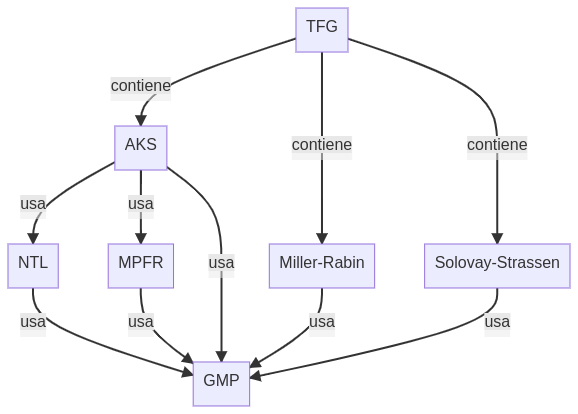
\includegraphics[totalheight=12cm]{img/diagrama-relaciones}
	\caption{Diagrama de relaciones de los componentes del proyecto}
\end{figure}

Todos los tests que se implementan en el proyecto hacen uso de la librería \textbf{GMP} para manejar números de precisión arbitraria. Además el algoritmo \textbf{AKS} hace uso de las librerías \textbf{NTL} (multiplicación de polinomios) y \textbf{MPFR} (cálculo preciso de cotas). Estas dos últimas además hacen uso de \textbf{GMP}. Finalmente tenemos el paquete \textbf{TFG} que incluye todos los tests de primalidad implementados. Ahor vamos a explicar cómo se ha estructurado físicamente el proyecto.\\

El código fuente está incluido todo en una carpeta a la que hemos llamado \textbf{TFG}. Dentro de esta carpeta tenemos varios archivos:

\begin{itemize}
	\item \textbf{.clang-tidy}: Control sobre los warnings que emite Clang-tidy.
	
	\item \textbf{suppressions.txt}: Control sobre los warnings que emite Cppcheck.
	
	\item \textbf{CMakeLists.txt}: Fichero con todas las órdenes necesarias para compilar el proyecto usando CMake.

	\item \textbf{conanfile.py}: Archivo Python donde se añaden las dependencias de Conan.
	
	\item \textbf{graphs.gp}: Archivo de \textbf{gnuplot} que usaremos para generar las gráficas comparativas de los tiempos de ejecución de los tests de primalidad.
\end{itemize}

Luego tenemos varias carpetas:

\begin{itemize}
	\item \textbf{include}: Cabeceras públicas de las funciones (API).
	
	\item \textbf{src}: Implementación de las funciones y cabeceras privadas.
	
	\item \textbf{tests}: Archivos con los tests unitarios.
	
	\item \textbf{examples}: Ejemplos para ejecutar los algoritmos implementados.
	
	\item \textbf{cmake}: Archivos auxiliares que usa el build system.
\end{itemize}

Todas las funciones de la librería se encuentran en un único namespace, llamado \textbf{tfg}, y en el archivo \textbf{include/TFG.hpp}.\\

Las funciones relativas al test \textbf{AKS} se encuentran en el namespace \textbf{tfg::aks}, y los pasos en el namespace \textbf{tfg::aks::steps}. La API se encuentra en el archivo \textbf{include/AKS.hpp}, y la implementación en \textbf{src/AKS.hpp}.\\

Las funciones que actúan como wrapper de las funciones de \textbf{GMP} están en el archivo \textbf{src/GMPWrappers.hpp} (no se exponen como parte de la librería) y las implementaciones en \textbf{src/GMPWrappers.cpp}. Todas estas funciones se encuentran en el namespace \textbf{tfg::gmp}.

\subsection{Comprobar potencia perfecta}

En este apartado vamos a presentar varias decisiones que se han tomado para implementar este algoritmo.\\

A pesar de que probamos que este algoritmo tiene complejidad $O^\sim(\log^4(n))$ y se presentará una posible implementación, la implementación final hará uso de la función ya implementada por la librería \textbf{GMP}.\\

Dicho esto, pasaremos a comprobar las distintas implementaciones.

\subsubsection{Implementación $O(\log^4(n))$}

En esta sección vamos a exponer de manera resumida el código en C++ necesario para implementar esta versión. Tampoco vamos a explicarlo mucho en profundidad, ya que en las siguientes secciones expondremos alternativas más eficientes y rápidas.\\

Primero presentamos la función \textit{isPowerOf}. Esta función toma dos valores $(n, p)$ y comprueba si existe algún $a$ tal que $n = a^p$.\\

\begin{lstlisting}
auto isPowerOf(mpz_class n, size_t p) -> bool {
	auto lower = 0_mpz;
	auto upper = n;
	
	while (lower <= upper) {
		auto middle = mpz_class{(lower + upper) / 2};
		auto value = pow(middle, p);
	
		if (value < n)
			lower = middle + 1;
		else if (value > n)
			upper = middle - 1;
		else
			return true;
	}
	
	return false;
}
\end{lstlisting}

La función puede ser optimizada un poco mejor si la primera cota de la cota superior (upper) es un poco más baja. Por ejemplo $2^{\lfloor \log(n)/p \rfloor + 1}$ sería válida, pero de momento la dejamos más simple.\\

El algoritmo es muy simple. Simplemente calculamos la mitad de ambas cotas, y ese número lo elevamos a $p$. Si el resultado es menor que $n$, actualizamos la cota inferior (lower); si es mayor, actualizamos la superior; y si es igual, devolvemos true. Si el bucle acaba, la búsqueda binaria no ha encontrado el valor, luego devolvemos false.\\

Ahora presentamos el algoritmo \textit{isPerfectPower}. Esta función toma un valor $n$ y comprueba si existen dos valores $a, p > 1$ tales que $n = a^p$.\\

\begin{lstlisting}
auto isPerfectPower(mpz_class n) -> bool {
	auto top = floorLog2(n);

	for (auto p = size_t{2}; p <= top; ++p)
		if (isPowerOf(n, p))
			return true;

	return false;
}
\end{lstlisting}

La función \textbf{floorLog2} se implementa como el número de bits que ocupa $n$ menos 1 (\textit{mpz\_sizeinbase(n.get\_mpz\_t(), 2) - 1}). Sabemos que ese es el top, y luego es simplemente comprobar para cada valor de $p$ si $n = a^p$ para algún $a > 1$.\\

Esta implementación es relativamente simple. Ahora pasaremos a explicar optimizaciones que podemos hacer a esta implementación para reducir la complejidad a $O^\sim(\log^3(n))$, tal y como se explica en \cite{bach_sorenson_1989}, Theorem 3.1.

\subsubsection{Implementación $O^\sim(\log^3(n))$}

En esta implementación simplemente realizaremos algunas pequeñas modificaciones a la anterior para poder reducir la complejidad.\\

En primer lugar, la primera optimización que haremos será reducir la primera cota superior en la función \textit{isPowerOf}. Por tanto, el único cambio es el siguiente:\\

\begin{lstlisting}
auto upper = pow(2_mpz, floorLog2(n) / p + 1);
\end{lstlisting}

De este modo, la complejidad de \textit{isPowerOf} pasa a ser $O(\log^3(n)/p)$, en contraste con la implementación del apartado anterior que era $O(\log^3(n))$. Ahora tenemos que optimizar la función \textit{isPerfectPower}.\\

Para ello, en vez de calcular una cota superior, simplemente vamos a usar el algoritmo de la Criba de Eratóstenes para calcular todos los primos menores que $\log(n)$. Suponiendo que tenemos dicho algoritmo implementado, la nueva versión quedaría tal que así:\\

\begin{lstlisting}
auto isPerfectPower(mpz_class n) -> bool {
	auto primes = eratosthenesSieve(floorLog2(n));
	
	for (auto prime : primes)
		if (isPowerOf(n, p))
			return true;
	
	return false;
}
\end{lstlisting}

La función \textit{eratostheneSieve} básicamente calcula todos los $p \in \N$ primos tales que $p \leq \lfloor \log(n) \rfloor$.\\

Luego simplemente iteramos cada primo y hacemos la comprobación con la búsqueda binaria.\\

Este algoritmo tiene complejidad $O^\sim(\log^3(n))$ \cite{bach_sorenson_1989}.

\subsubsection{Implementación GMP}

La versión que finalmente se ha implementado es la que ya proporciona la librería \textbf{GMP}. Dicha función se llama \textit{mpz\_perfect\_power\_p}. Recibe un único argumento $n$ de tipo \textit{mpz\_t} y devuelve un entero distinto de $0$ si $n$ es una potencia perfecta.\\

La función se ha encapsulado en su correspondiente wrapper llamado \textbf{isPerfectPower} en el namespace \textbf{tfg::gmp}. La implementación es la siguiente:\\

\begin{lstlisting}
auto isPerfectPower(mpz_class const& n) -> bool {
	return mpz_perfect_power_p(n.get_mpz_t()) != 0;
}
\end{lstlisting}

Este algoritmo utiliza el método de Newton para calcular raíces. Una explicación un poco más detallada se puede encontrar en el Apéndice.

\subsection{Encontrar menor $r$ tal que $ord_r(n) > \log^2(n)$}

En este paso vamos a calcular el valor de $r$ que luego usaremos en el paso 5. Explicaremos tanto la manera en que calculamos la cota como el cálculo de $ord_r(n)$ de manera eficiente.

\subsubsection{Calcular $\log^2(n)$}

Para calcular esta cota de manera fiable y lo más baja posible, usaremos la librería \textbf{MPFR}, ya que con \textbf{GMP} no podemos asegurar una cota tan precisa. Para calcular la cota, este es el código:\\

\begin{lstlisting}
auto log2Sqr(mpz_class n) -> size_t {
	mpfr_t thresholdMPFR;
	mpfr_init_set_z(thresholdMPFR, n.get_mpz_t(), MPFR_RNDU);
	mpfr_log2(thresholdMPFR, thresholdMPFR, MPFR_RNDU);
	mpfr_sqr(thresholdMPFR, thresholdMPFR, MPFR_RNDU);
	
	return mpfr_get_ui(thresholdMPFR, MPFR_RNDD);
}
\end{lstlisting}

Primero cabe destacar que la cota no debería sobrepasar los 64 bits de capacidad (pues luego tendremos que reservar memoria acorde a esta cota), luego podemos devolver un entero sin signo cuyo valor máximo nunca será menor que la cantidad de memoria del ordenador.\\

Primero inicializamos una variable de tipo \textit{mpfr\_t} (número en coma flotante con precisión arbitraria) con la función \textit{mpfr\_init\_set\_z}, que toma nuestro entero de \textbf{GMP} y lo redondea hacia $+\infty$.\\

Después realizamos \textit{mpfr\_log2} y \textit{mpfr\_sqr} sucesivamente, que son las funciones logaritmo en base $2$ y elevar al cuadrado respectivamente (todo esto reutilizando la misma memoria). Seguimos redondeando a $+\infty$.\\

Finalmente devolvemos la cota que hemos calculado en coma flotante como si fuera un entero redondeado hacia $-\infty$ (o lo que es lo mismo, $\lfloor \log_2(n)^2 \rfloor$).

\subsubsection{Comprobar que $ord_r(n) > \log^2(n)$}

Para este paso, como ya explicamos anteriormente, no necesitamos calcular explícitamente $ord_r(n)$, sino simplemente comprobar que $n^k \neq 1 \mod(r)$ para todo $k \leq \log^2(n)$. Este es el código:\\

\begin{lstlisting}
auto isOrderBiggerThan(mpz_class n, size_t r, size_t threshold) -> bool {
	auto temp = 1_mpz;
	
	for (auto i = std::size_t{1}; i <= threshold; ++i) {
		temp *= n;
		temp %= r;
		
		if (temp == 1)
			return false;
	}
	
	return true;
}
\end{lstlisting}

Las entradas son $n$ (número cuya primalidad queremos testear), $r$ (el valor actual que estamos comprobando) y threshold (cota previamente calculada).\\

Es importante remarcar que, aunque sabemos que la cota es $\log^2(n)$ y, por lo tanto, podríamos calcularla dentro del bucle, es preferible calcularla fuera una vez y pasarla simplemente a esta función cada vez.\\

El algoritmo es muy simple. Simplemente comprobamos si en algún momento $n^k = 1 \mod(r)$ y, en dicho caso, devolver false (pues el orden entonces es menor que la cota que hemos pasado).\\

Si acabamos el bucle, significa que $ord_r(n) > \log^2(n)$, luego devolvemos true.

\subsubsection{Bucle para probar valores de $r$}

Con las dos funciones anteriores, estamos preparados para ejecutar el segundo paso. Este es el código:\\

\begin{lstlisting}
auto step2(mpz_class n) -> size_t {
	auto const threshold = log2Sqr(n);
	
	for (auto r = threshold + 2;; ++r)
		if (isOrderBiggerThan(n, r, threshold))
			return r;
}
\end{lstlisting}

Lo importante a destacar aquí es que el primer $r$ que probamos es $\log^2(n) + 2$, pues este es el primer $r$ para el que es posible que se cumpla que $ord_r(n) > \log^2(n)$.\\

La razón es simplemente que, dado que $n^{\phi(r)} \equiv 1 \mod(r)$ para todo $n, r \geq 1$, si $r \leq \log^2(n) + 1 \Rightarrow ord_r(n) \leq \phi(r) \leq r - 1 \leq \log^2(n)$, luego sería imposible que $ord_r(n) > \log^2(n)$.\\

Más allá de esa aclaración, el código es simple. Simplemente vamos probando hasta que encontremos el $r$ que cumple la condición, el cual ya sabemos que existe por \autoref{cota_superior_r_log5}.

\subsection{Comprobar si $1 < (a, n) < n$ para algún $a \leq r$}

Este paso es bastante sencillo, pues solo tenemos que calcular el máximo común divisor repetidamente para valores de $a \leq r$. El código para ello es bastante simple:\\

\begin{lstlisting}
auto checkGCD(mpz_class n, size_t r) -> bool {
	for (auto a = size_t{2}; a <= r; ++a) {
		auto const result = gmp::gcd(a, n);
	
		if (1 < result && result < n)
			return true;
	}
	return false;
}
\end{lstlisting}

Como dijimos anteriormente, usamos \textbf{size\_t}/\textbf{std::size\_t} para el tipo de $r$ (pues luego lo usaremos para reservar memoria).\\

La función \textit{gmp::gcd} simplemente es un wrapper de la función de \textbf{GMP}, el cual ya explicamos al principio de este capítulo.\\

Si encontramos un $a$ de manera que $1 < (a, n) < n$, devolvemos true. En caso contrario, devolvemos false.

\subsection{Comprobar si $n \leq r$}

Este paso sea probablemente el más fácil de todos, y ocupará poco espacio en nuestro análisis.\\

En este paso simplemente tendremos que añadir un condicional tal que así entre los pasos 3 y 5:\\

\begin{lstlisting}
if (n <= r)
	return true;
\end{lstlisting}

Podemos optimizar esto un poco más si tenemos en cuenta que este paso solo es necesario, ya que la condición $n \leq r$ solo se cumple si $n \leq 5'690'034$, pues $\lceil \log^5(r) \rceil < r$ para todo $n > 5'690'034$.\\

Esta optimización puede ser útil cuando el número de cifras crezca mucho, aunque tampoco va a afectar mucho, pues volvemos a insistir que la complejidad real está en el paso 5.

\subsection{Comprobar identidades polinómicas}

Este apartado será en el que invirtamos más tiempo, pues es en el que realmente tenemos que optimizar donde sea posible para poder tener un tiempo de ejecución razonable.\\

Lo 4 pasos anteriores no suponen ningún problema de eficiencia con números relativamente grandes. El tener que manejar memoria en este paso puede suponer un auténtico problema si no lo hacemos adecuadamente, pues muchas reservas de memoria pueden resultar en un tiempo de ejecución muy lejos de lo que aspiramos conseguir.\\

En este apartado discutiremos 2 implementaciones posibles. Cada una tiene sus ventajas e inconvenientes, los cuales detallaremos a continuación:\\

\begin{itemize}
	\item \textbf{Implementación directa}. Esta implementación es la más directa, sencilla de integrar en el código fuente (ya que no hace uso de librerías externas) y la que nos da más flexibilidad al tomar distintas decisiones.\\
	
	La mayor desventaja es que será muy complicado lograr una eficiencia parecida a la que otras librerías ya han conseguido, pues mientras que esta implementación se puede realizar en un par de días o tres de desarrollo, optimizarla puede suponer un tiempo innecesariamente largo.\\
	
	Además de lo mencionado, para que el algoritmo sea realmente rápido, habría que implementar la versión de la multiplicación polinómica que hace uso de la \textit{Transformada Rápida de Fourier} (FFT). En nuestro caso usaremos el método clásico para no perder excesivo tiempo en dicha implementación y centrarnos más en las que nos proporciona la librería siguiente.
	
	\item \textbf{NTL}. Esta librería ya tiene implementadas funciones para poder trabajar con anillos de polinomios y módulos, además de haber sido optimizada. Además, la interfaz es en C++, lo cual facilita su integración.\\
	
	Sin embargo esta librería no viene incluida con el manejador de paquetes de Conan, por lo que será necesario instalar dicha librería en el sistema o compilarla a mano, lo cual puede resultar engorroso para el usuario final.
\end{itemize}

Dicho esto, empecemos con el análisis de la implementación del paso 5.

\subsubsection{Cálculo de cota superior para el bucle}

La primera parte del paso es calcular el valor para saber cuántas iteraciones tenemos que realizar. Esta cota es $\lfloor \sqrt{\phi(r)}\log(n) \rfloor$. Para ello, recurriremos de nuevo a la librería \textbf{MPFR} para conseguir una cota lo más fiel y baja posible.\\

Primero necesitamos una implementación para la función $\phi$ de Euler, la cual podemos ver en el siguiente código. Aquí no usamos el tipo de \textbf{GMP}, pues sabemos que $r$ cabe en el tipo \textit{size\_t}:\\

\begin{lstlisting}
auto phi(size_t n) -> size_t {
	auto const top = size_t{std::sqrt(n)};
	auto result = n;

	for (auto p = size_t{2}; p <= top; ++p) {
		if (n % p == 0) {
			while (n % p == 0)
				n /= p;
	
			result -= result / p;
		}
	}
	
	if (n > 1)
		result -= result / n;
	
	return result;
}
\end{lstlisting}

Esta función es una implementación sencilla que simplemente va calculando el valor de $\phi(n)$ a medida que va factorizando $n$. Esta implementación además evita el uso de números en coma flotante, lo cual ayuda a obtener resultados exactos sin recurrir a aproximaciones.\\

Ahora pasamos a explicar la función que calcula la cota. El código para ello es el siguiente:\\

\begin{lstlisting}
auto upperBoundStep5(mpz_class n, size_t r) -> size_t {
	mpfr_t result;
	mpfr_init_set_z(result, n.get_mpz_t(), MPFR_RNDU);
	mpfr_log2(result, result, MPFR_RNDU);
	
	mpfr_t sqrtPhiR;
	mpfr_init_set_ui(sqrtPhiR, phi(r), MPFR_RNDU);
	mpfr_sqrt(sqrtPhiR, sqrtPhiR, MPFR_RNDU);
	
	mpfr_mul(result, result, sqrtPhiR, MPFR_RNDU);
	
	return mpfr_get_ui(result, MPFR_RNDD);
}
\end{lstlisting}

Empezamos calculando $\log(n)$, lo cual lo hacemos fácilmente con las tres primeras líneas. Para ello inicializamos una variable de tipo \textit{mpfr\_t} con $n$ (\textbf{MPFR} admite conversiones desde tipos de \textbf{GMP}) y luego usamos \textit{mpfr\_log2} para aplicarle el logaritmo en base $2$ y así obtener $\log(n)$.\\

Lo siguiente es calcular $\sqrt{\phi(r)}$ en las tres siguientes líneas. Inicializamos otra variable de tipo \textit{mpfr\_t} con el valor de llamar a la función \textit{phi} con $r$, teniendo así $\phi(r)$. Ahora usamos la función \textit{mpfr\_sqrt} para calcularle la raíz cuadrada, obteniendo así $\sqrt{\phi(r)}$.\\

Después calculamos $\sqrt{\phi(r)}\log(n)$ usando la función \textit{mpfr\_mul} y acumulando el resultado en la primera variable que creamos (para no reservar más memoria).\\

Finalmente devolvemos $\lfloor \sqrt{\phi(r)}\log(n) \rfloor$ usando el resultado de la llamada a \textit{mpfr\_get\_ui}, que devuelve el valor del resultado como un entero sin signo y redondeando hacia $-\infty$.\\

Ahora vamos a pasar a explicar las implementaciones del bucle principal del algoritmo. Es solo esta parte en la que divergen varias implementaciones en todo el algoritmo. Esta separación nos servirá luego para poder comparar ambas implementaciones y ver las ventajas de una sobre la otra.\\

Destacar que ambas implementaciones residen en el namespace \textbf{tfg::aks::steps::impl} y están expuestas públicamente. La primera se llama \textit{step5Direct}, y la segunda \textit{step5NTL}. En la implementación final se usa por defecto la segunda por ser más eficiente.

\subsubsection{Bucle: Implementación Directa}

Ahora vamos a centrarnos en cómo podríamos hacer una implementación directa sin hacer uso de librerías externas para el bucle principal del algoritmo \textbf{AKS}.\\

Para ello necesitamos implementar la operación principal de la identidad: exponenciación rápida de un polinomio módulo otro polinomio y un entero. Esta operación puede parecer aparentemente sencilla, pero requiere de un buen manejo de la memoria para no estar reservando memoria constantemente en cada iteración del bucle.\\

Vamos a presentar entonces dos clases que nos ayudarán a la hora de la implementación:

\begin{itemize}
	\item \textbf{AKSCoefficient}: Esta clase es simplemente un wrapper de \textit{mpz\_class} para trabajar con aritmética modular más fácilmente.\\
	
	El único atributo de dichos objetos es una variable de tipo \textit{mpz\_class}, donde las operaciones de suma, resta y multiplicación se han adaptado al anillo $\Z_n$.\\
	
	Además, para que todos los objetos de dicha clase tengan el mismo módulo, se ha añadido una variable estática de clase (común a todos los objetos) que indicará el anillo en el que nos encontramos.
	
	\item \textbf{AKSPolynomial}: Esta clase representa un polinomio con coeficientes en $\Z_n$ y módulo $X^r - 1$ o, dicho de otro modo, el anillo $\Z_n[X]/(X^r - 1)$. Agruparlo así nos servirá para controlar mejor el uso de memoria.\\
	
	Consta de tres atributos:
	
	\begin{itemize}
		\item Dos buffers de tamaño $2r$. Uno para almacenar los coeficientes del polinomio. El otro es un buffer auxiliar que nos servirá para evitar reservas de memoria repetidas cada vez que hagamos una operación sobre los polinomios.
		
		\item Un entero sin signo indicando el grado actual del polinomio.
	\end{itemize}
	
	Además, hay una variable estática de clase que indicará el grado del polinomio que marca el módulo (si el polinomio es $X^r - 1$, nosotros guardamos el valor de $r$).
\end{itemize}

Ambas clases son extremadamente simples en el sentido de que implementaremos lo justo para poder usarlas con el algoritmo \textbf{AKS}, y además no estarán expuestas en la interfaz pública, por lo que no necesitamos una API extremadamente versátil.\\

La implementación de \textbf{AKSCoefficient} es simplemente un wrapper con las operaciones elementales adaptadas al anillo $\Z_n$, por lo que no vamos a ocupar mucho tiempo en ella.\\

Decir que los operadores que se implementan son +=, -= y *=. Esto es para evitar que se hagan muchas reservas de memoria y simplemente actualizar los valores. Además se implementa el operador == para poder comparar dos objetos de esta clase, constructores que aceptan variables de tipo \textit{mpz\_class} y una pareja getter/setter para cambiar el módulo del anillo, es decir, indicar en qué $\Z_n$ estamos.\\

La clase \textbf{AKSPolynomial} es la que va a hacer el trabajo pesado, pues es la que se va a encargar de implementar las operaciones polinómicas. Vamos a indicar varias características de esta clase:

\begin{itemize}
	\item Una característica importante de esta clase es que no se puede copiar. Tiene el constructor y la asignación por copia eliminados explícitamente. Esto nos va a ayudar a que no se hagan copias accidentalmente.
	
	\item Tiene un constructor que acepta dos variables de tipo \textbf{AKSCoefficient}, que indican los dos primeros coeficientes. Esto es porque en el algoritmo solo necesitamos construir polinomios de esa manera y no con tantos coeficientes como queramos.
	
	\item Los únicos operadores que se implementan son -= y *=. El primero acepta una variable de tipo \textbf{AKSCoefficient} (básicamente restar un escalar al polinomio). El segundo acepta otro polinomio, y es donde se implementará la operación de multiplicación de polinomios.
	
	\item Se implementa la operación \textit{pow}, que acepta una variable de tipo \textit{mpz\_class} y eleva el polinomio a dicho valor. Además acepta un segundo parámetro que es donde se guardará el resultado de la operación (esto con el fin de evitar reservar memoria repetidas veces).
\end{itemize}

Empezamos viendo la operación \textit{pow}. El código es el siguiente:\\

\begin{lstlisting}
auto AKSPolynomial::pow(mpz_class exp, AKSPolynomial& result) const -> void {
	result.setCoefficient(0, 1_mpz);
	result.m_currentDegree = 0;
	
	for (auto const& bit : exp.get_str(2))
	{
		result *= result;
		if (bit == '1')
			result *= *this;
	}
}
\end{lstlisting}

El algoritmo simplemente va tomando los bits del número que se le pasa con la función \textit{get\_str}. Los bits se recorren de más significativo a menos. Simplemente elevamos al cuadrado en cada iteración el resultado y, si el bit es $1$, multiplicamos por el valor que estamos elevando. Este algoritmo es bien conocido y realiza $O(\log(n))$ multiplicaciones.\\

Ahora vamos a presentar una función auxiliar, \textit{adjustDegree}, que sirve para adaptar el grado del polinomio:\\

\begin{lstlisting}
auto AKSPolynomial::adjustDegree() -> void {
	while (getCoefficient(getDegree()) == 0_mpz && getDegree() > 0)
		--m_currentDegree;
}
\end{lstlisting}

Las funciones \textit{getCoefficient} y \textit{getDegree} son getters para obtener un coeficiente específico y obtener el grado del polinomio respectivamente.\\

Simplemente va actualizando el grado del polinomio hasta que se encuentra un coeficiente distinto de $0$ o llega al grado $0$.\\

La siguiente operación que vamos a presentar es la división del polinomio por el módulo:\\

\begin{lstlisting}
auto AKSPolynomial::dividePolMod() -> void {
	if (getDegree() >= getModuleDegree()) {
		for (auto i = getDegree(); i >= getModuleDegree(); --i)
			m_coeffs[i - getModuleDegree()] += getCoefficient(i);
		
		m_currentDegree = getModuleDegree() - 1;
	}
	adjustDegree();
}
\end{lstlisting}

Antes de explicar la función, destacar que la función \textit{getModuleDegree} devuelve el grado del polinomio $X^r - 1$, pues para el algoritmo no necesitamos el polinomio entero y podemos realizar ciertas optimizaciones basadas en ello. La variable \textit{m\_coeffs} es el buffer que contiene los coeficientes.\\

Básicamente, lo que hacemos es aplicar el algoritmo clásico de división de polinomios. Como sabemos que el polinomio siempre es de la forma $X^r - 1$, podemos simplemente actualizar los $n - r$ primeros coeficientes desde el de más grado hasta el de menos. Finalmente reajustamos el grado del polinomio resultante. De este modo, la eficiencia es $O(n - r)$ o $O(r)$ teniendo en cuenta que el polinomio siempre será de grado $O(r)$.\\

Finalmente vamos a presentar la multiplicación. Cabe destacar que aquí usamos el algoritmo elemental. Para conseguir una mejor eficiencia será necesario usar la versión que hace uso de la \textit{Transformada Rápida de Fourier}. Esto no lo haremos aquí ya que puede ser complicado implementarla correctamente y las próximas versiones ya harán ese trabajo por nosotros.\\

\begin{lstlisting}
auto AKSPolynomial::operator*=(AKSPolynomial const& rhs) -> AKSPolynomial& {
	auto const newDegree = getDegree() + rhs.getDegree() + 1;
	
	for (auto i = std::size_t{0}; i <= newDegree; ++i)
		m_coeffsAux[i] = 0_mpz;
	
	for (auto i = std::size_t{0}; i <= getDegree(); ++i) {
		for (auto j = std::size_t{0}; j <= rhs.getDegree(); ++j) {
			auto product = getCoefficient(i);
			product *= rhs.getCoefficient(j);
			m_coeffsAux[i + j] += product;
		}
	}
	
	m_currentDegree = newDegree;
	std::swap(m_coeffs, m_coeffsAux);
	
	dividePolMod();
	
	return *this;
}
\end{lstlisting}

Explicamos cada paso con detalle:

\begin{enumerate}
	\item Primero calculamos el grado final del polinomio resultante (la suma de ambos grados más $1$).
	
	\item Actualizamos los valores del buffer auxiliar, \textit{m\_coeffsAux} a $0$ (preparando el terreno para acumular el resultado).
	
	\item Bucle doble donde básicamente aplicamos el algoritmo elemental de multiplicación de polinomios y acumulamos el resultado en el buffer auxiliar.
	
	\item Actualizamos el grado del polinomio actual al del producto.
	
	\item Intercambiamos los buffers, de modo que el buffer principal contenga el resultado de la multiplicación.
	
	\item Finalmente aplicamos la división por el módulo, la cual ya ajusta el grado del resultado final.
\end{enumerate}

La parte que deberíamos optimizar es el bucle anidado donde realizamos el algoritmo de multiplicación, pero no lo haremos en este apartado ya que será complicado hacerlo correctamente.\\

Finalmente, y haciendo uso de lo que acabamos de explicar, podemos implementar el quinto paso de la siguiente manera:\\

\begin{lstlisting}
auto step5Direct(mpz_class n, size_t r) -> bool {
	auto const top = calculateUpperBound(n, r);
	
	detail::AKSCoefficient::setModule(n);
	detail::AKSPolynomial::setModuleDegree(r);
	
	auto lhs = detail::AKSPolynomial{};
	auto rhs = detail::AKSPolynomial{};
	
	auto temp = detail::AKSPolynomial{0_mpz, 1_mpz};
	
	temp.pow(detail::AKSCoefficient::getModule(), rhs);
	
	for (auto a = std::size_t{1}; a <= top; ++a) {
		temp.setCoefficient(0, mpz_class{a});
		temp.pow(detail::AKSCoefficient::getModule(), lhs);
		lhs -= mpz_class{a};
		
		if (lhs != rhs)
			return true;
	}
	
	return false;
}
\end{lstlisting}

Antes de explicar cada paso en detalle, es importante aclarar que la identidad que vamos a comprobar la vamos a modificar ligeramente. En vez de comprobar $(X + a)^n \equiv X^n + a \mod(X^r - 1, n)$, vamos a comprobar $(X + a)^n - a \equiv X^n \mod(X^r - 1, n)$. Esto nos permite evitar calcular el polinomio de la parte derecha en cada iteración, ya que no dependerá de la variable de iteración $a$. Ahora explicamos en detalle cada paso:

\begin{enumerate}
	\item Primero calculamos la cota del bucle con la función \textbf{calculateUpperBound}.
	
	\item Indicamos a las clases el módulo $(X^r - 1, n)$ en el que vamos a trabajar.
	
	\item Creamos los dos polinomios que usaremos para comprobar las identidades: \textit{lhs} para $(X + a)^n - a$ y \textit{rhs} para $X^n$. Además creamos uno extra que nos servirá para almacenar el resultado de elevar la parte izquierda y no reservar memoria repetidas veces.
	
	\item Almacenamos en \textit{rhs} el resultado de $X^n \mod(X^r - 1, n)$.
	
	\item Empezamos el bucle, y en cada iteración, almacenamos en \textit{lhs} el resultado de $(X + a)^n - a \mod(X^r - 1, n)$. Comparamos \textit{lhs} con \textit{rhs}, y devolvemos true si no coinciden.
	
	\item Si llegamos al final del bucle, devolvemos false (Es decir, que se han cumplido las identidades).
\end{enumerate}

La complejidad de esta implementación está entre $O^\sim(\log^8(n))$ y $O^\sim(\log{31/2}(n))$ (según el valor de $r$). Esto se debe a que la multiplicación de enteros viene dada por la librería \textbf{GMP}, que implementa la dicha operación con complejidad $O^\sim(\log(n))$; y porque el algoritmo de multiplicación de polinomios implementado sin uso de librerías externas es $O^\sim(r^2\log(n))$.

\subsubsection{Bucle: Implementación con NTL}

En este apartado nos vamos a centrar en implementar el paso 5 haciendo uso de la librería \textbf{NTL}.\\

Esta implementación hace uso de algoritmos para realizar la multiplicación de polinomios con complejidad $O^\sim(nm)$ en vez de $O^\sim(n^2m)$, como en el apartado anterior.\\

Presentamos entonces una implementación del paso 5 haciendo uso de la librería \textbf{NTL}:\\

\begin{lstlisting}
auto step5NTL(mpz_class n, size_t r) -> bool {
	auto const top = calculateUpperBound(n, r);
	
	auto const nNTL = NTL::conv<NTL::ZZ>(n.get_str().c_str());
	NTL::ZZ_p::init(nNTL);
	
	auto const module = NTL::ZZ_pXModulus{NTL::ZZ_pX{r, 1} - 1};
	
	auto const rhs = [&nNTL, &module] {
		auto result = NTL::ZZ_pX{1, 1};
		NTL::PowerMod(result, result, nNTL, module);
		
		return result;
	}();
	
	for (auto a = std::size_t{1}; a <= top; ++a) {
		auto lhs = NTL::ZZ_pX{1, 1};
		lhs += a;
		NTL::PowerMod(lhs, lhs, nNTL, module);
		lhs -= a;
		
		if ((lhs != rhs) != 0)
			return true;
	}
	
	return false;
}
\end{lstlisting}

Primero, al igual que en la implementación anterior, calculamos la cota superior del bucle haciendo uso de la función \textit{calculateUpperBound}.\\

Después convertimos la entrada (entero de \textbf{GMP}, \textit{mpz\_class}) a un entero de \textbf{NTL}, \textit{NTL::ZZ}, para poder usarlo en los algoritmos de esta librería. Hecho eso, inicializamos el módulo $\Z_n$ con la llamada a \textit{NTL::ZZ\_p::init}. Esto hará que todas las operaciones en enteros sean módulo $n$.\\

Ahora declaramos el polinomio $X^r - 1$ como el módulo que usaremos para exponenciar.\\

Después calculamos $X^n \mod(X^r-1, n)$ con la función \textit{NTL::PowMod}. El segundo parámetro es el polinomio a exponenciar (base). El tercer parámetro es el exponente. El cuarto parámetro es el polinomio cuyo módulo vamos a aplicar.El resultado se guarda en el primer parámetro.\\

Finalmente ejecutamos el bucle, y en cada iteración calculamos $(x + a)^n - a \mod(X^r-1, n)$. Si alguna identidad no se cumple, devolvemos true.\\

Finalmente, si llegamos al final del bucle, devolvemos false (pues todas las identidades se han cumplido).\\

La complejidad de esta implementación está entre $O^\sim(\log^6(n))$ y $O^\sim(\log{21/2}(n))$ (según el valor de $r$). Esto se debe a que la multiplicación de enteros viene dada por la librería \textbf{GMP}, que implementa la dicha operación con complejidad $O^\sim(\log(n))$; y porque el algoritmo de multiplicación de polinomios implementado por \textbf{NTL} tiene complejidad $O^\sim(r\log(n))$.

\subsection{Paso 6: Devolver true}

Este paso simplemente se implementa como una función a parte para ser más fiel al algoritmo original y estar en concordancia con el resto de pasos. Consiste en una función que devuelve true.

\section{Comparación Implementación Directa/NTL}

En esta sección vamos a justificar con resultados gráficos la elección de usar la librería externa \textbf{NTL} a la hora de elegir una implementación definitiva del paso $5$ del algoritmo \textbf{AKS}.\\

Como ya explicamos anteriormente, este paso es el único en el que usamos implementaciones distintas, por lo que el resto de pasos serán comunes en la comparación y solo mediremos el tiempo de ejecución del quinto paso.\\

Para la comparación vamos a usar los mayores primos que ocupan una cantidad determinada de bits (desde $2$ bits hasta $13$ bits). Nuestro conjunto de prueba será el siguiente:

\[ \{ 3, 7, 13, 31, 61, 127, 251, 509,
1021, 2039, 4093, 8191, 16381, 32749,
65521 \} \]

No usamos primos más grandes porque, como veremos en las gráficas, el tiempo que invierte la implementación directa es muy alto para números pequeños.\\

No usamos números compuestos porque necesitamos comparar la eficiencia del paso $5$, el cual se ejecuta por completo cuando la entrada se trata de un número primo. Es por ello que aquí no tiene mucho sentido usar números compuestos. Por esta razón, en la comparación solo vamos a ejecutar los pasos $2$ y $5$, ya que necesitamos el valor de $r$ calculado en el segundo paso para poder ejecutar el quinto.

Además de presentar los tiempos de ejecución de ambas implementaciones, también vamos a representar las gráficas de las eficiencias teóricas ajustadas con la función \textit{fit} de \textit{gnuplot}.\\

Ambos ejes de las gráficas están en escala logarítmica en base $2$, para que se puedan apreciar mejor los resultados.\\

Esta gráfica muestra los tiempos de ejecución de la implementación directa junto con sus eficiencias teóricas.

\begin{figure}[H]
	\centering
	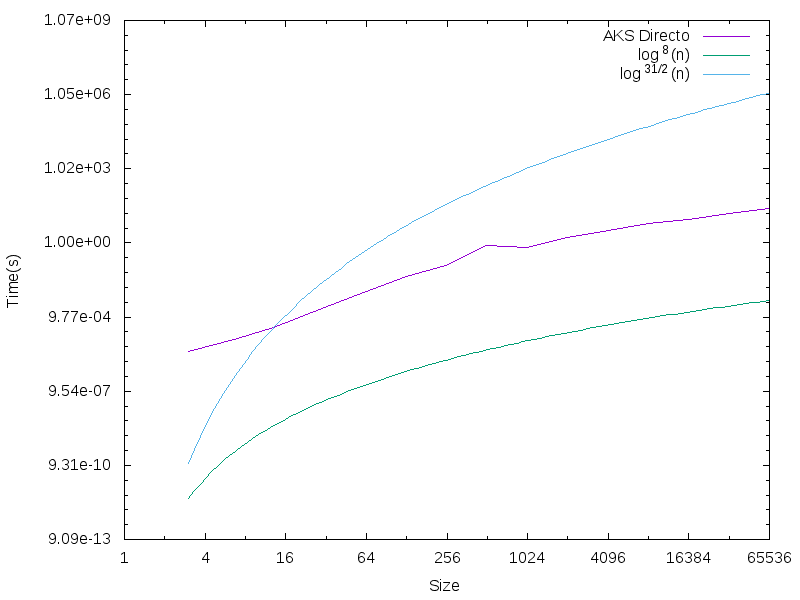
\includegraphics[totalheight=12cm]{img/graphs/aks-direct-mean}
	\caption{Gráfica AKS con implementación directa}
\end{figure}

Esta gráfica muestra los tiempos de ejecución de la implementación usando \textbf{NTL} junto con sus eficiencias teóricas.

\begin{figure}[H]
	\centering
	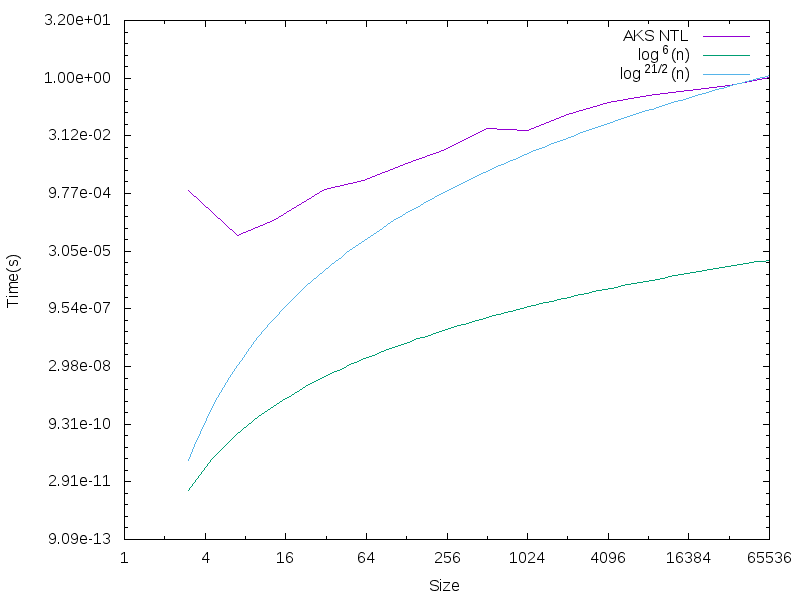
\includegraphics[totalheight=12cm]{img/graphs/aks-ntl-mean}
	\caption{Gráfica AKS usando NTL}
\end{figure}

Finalmente mostramos la comparación de ambas implementaciones.

\begin{figure}[H]
	\centering
	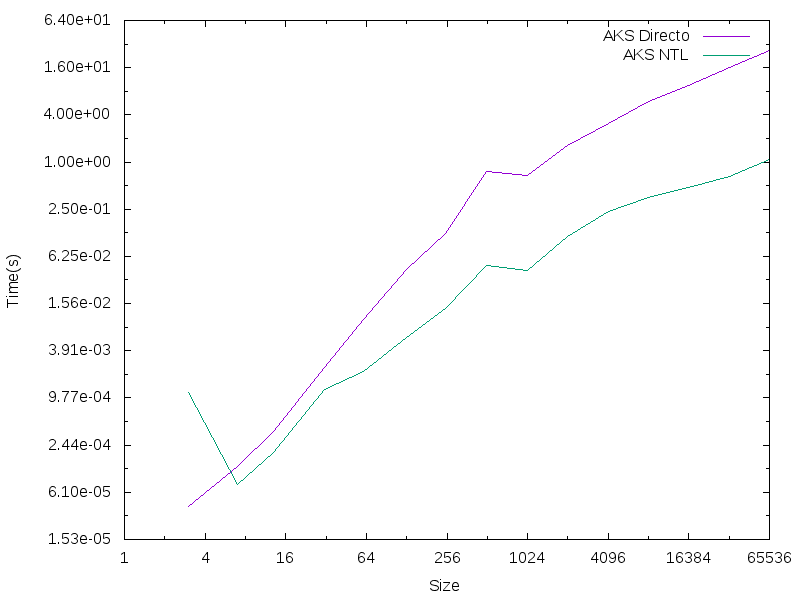
\includegraphics[totalheight=12cm]{img/graphs/aks-mean}
	\caption{Comparación ambas implementaciones AKS}
\end{figure}

Como podemos comprobar, el tiempo de ejecución de la implementación directa es mucho mayor que la implementación usando la librería \textbf{NTL}. Esto es debido al algoritmo de multiplicación polinómica usado en ambos casos, lo cual resalta su importancia a la hora de implementar el algoritmo \textbf{AKS}.\\

Puesto que la implementación usando \textbf{NTL} es superior, será la que usaremos en el siguiente apartado para comparar el algoritmo \textbf{AKS} con los tests probabilísticos de \textit{Miller-Rabin} y \textit{Solovay-Strassen}.

\endinput
%------------------------------------------------------------------------------------
% FIN DEL CAPÍTULO. 
%------------------------------------------------------------------------------------

% !TeX root = ../libro.tex
% !TeX encoding = utf8
\chapter{Comparación con algoritmos probabilísticos}

En este capítulo vamos a implementar algunos tests de primalidad probabilísticos para poder comparar su tiempo de ejecución con la implementación descrita anteriormente del test \textbf{AKS}.\\

En específico, vamos a implementar dos tests: \textit{Miller-Rabin} y \textit{Solovay-Strassen}. Una vez implementados estos dos tests, haremos varias comparaciones con el test \textbf{AKS} usando distintos conjuntos de números:

\begin{itemize}
	\item Números primos.
	\item Potencias de primos.
	\item Números compuestos no potencias de primos.
\end{itemize}

El análisis de cada conjunto irá acompañado de gráficas que representen visualmente los tiempos de ejecución de los distintos tests. Para cada conjunto analizaremos los resultados correspondientes y sacaremos conclusiones respecto a la eficiencia de cada test.

\section{Tests Probabilísticos}

En esta sección vamos a presentar las dos implementaciones de los tests probabilísticos que vamos a usar, además de explicarlos un poco por encima.\\

La base teórica de ambos test ya la explicamos anteriormente, y en esta solo nos vamos a centrar en la implementación de los mismos.\\

En ambos casos, la entrada consiste de tres parámetros, descritos a continuación en el mismo orden:

\begin{enumerate}
	\item Número cuya posible primalidad queremos comprobar.
	\item Número de rondas del test probabilístico a realizar.
	\item (Opcional) Generador de números aleatorio. Esto puede ser útil a la hora de testear el código de manera determinista. En caso de que no se pase ninguno, se usará uno con una semilla generada aleatoriamente.
\end{enumerate}

\subsection{Test de Miller-Rabin}

Ahora vamos a presentar una implementación del test de \textit{Miller-Rabin}. Dicha implementación está expuesta públicamente y se encuentra en el namespace \textit{tfg::miller\_rabin}:\\

\begin{lstlisting}
auto isProbablyPrime(mpz_class n, mpz_class k, gmp_randclass &prng) -> bool {
	if (n == 2_mpz || n == 3_mpz)
		return true;
	
	if (n < 2 || n % 2 == 0)
		return false;
	
	auto const [r, d] = [&n] {
		auto dResult = mpz_class{n - 1};
		auto rResult = mpz_scan1(dResult.get_mpz_t(), 0);
		mpz_fdiv_q_2exp(dResult.get_mpz_t(), dResult.get_mpz_t(), rResult);
		
		return std::make_pair(rResult, dResult);
	}();
	
	for (auto i = 0_mpz; i < k; ++i) {
		auto const a = mpz_class{prng.get_z_range(n - 3) + 2};
		auto x = gmp::powMod(a, d, n);
		
		if (x != 1 && x != n - 1) {
			for (auto j = 0_mpz; j < r - 1; ++j) {
				x = gmp::powMod(x, 2, n);
				
				if (x == n - 1)
					break;
			}
			
			if (x != n - 1)
				return false;
		}
	}
	
	return true;
}
\end{lstlisting}

Primero nos libramos de los múltiplos de dos con las dos primeras condiciones. Además manejamos el caso $n = 3$ para asegurar que el test de \textit{Miller-Rabin} solo lo aplicamos a enteros impares mayores que $3$.\\

Después encontramos $r, d$ tales que $n = 2^rd + 1$.\\

Después ejecutamos el test de \textit{Miller-Rabin} el número de rondas que le hemos pasado y, para cada ronda, generamos un número aleatorio entre $2$ y $n-2$ (ambos inclusive), el cual usaremos para comprobar las congruencias \eqref{congruencias_miller_rabin}.\\

Si en alguna ronda no se pasa el test, se devuelve false (el número es compuesto). Si llegamos al final del bucle, entonces devolvemos true (el número es probablemente primo).

\subsection{Test de Solovay-Strassen}

Ahora vamos a presentar una implementación del algoritmo de Solovay-Strassen. Dicha implementación está expuesta públicamente y se encuentra en el namespace \textit{tfg::solovay\_strassen}:\\

\begin{lstlisting}
auto isProbablyPrime(mpz_class n, mpz_class k, gmp_randclass &prng) -> bool {
	if (n == 2)
		return true;
	
	if (n < 2 || n % 2 == 0)
		return false;
	
	for (auto i = 0_mpz; i < k; ++i) {
		auto const a = mpz_class{prng.get_z_range(n - 2) + 2};
		auto const x = [&a, &n] {
			auto result = gmp::jacobiSymbol(a, n);
			return (result < 0) ? n + result : result;
		}();
		
		if (x == 0 || gmp::powMod(a, (n - 1)/2, n) != x)
			return false;
	}
	
	return true;
}
\end{lstlisting}

Primero nos libramos de los múltiplos de $2$.\\

Una vez hecho eso, simplemente ejecutamos el test el número de rondas que se ha pasado con números aleatorios generados entre $2$ y $n-1$. El \textit{Símbolo de Jacobi} \ref{simbolo_de_jacobi} lo hayamos usando la función que nos proporciona \textbf{GMP} para ello (usando el wrapper que hemos creado para C++).\\

Igual que con el test de \textit{Miller-Rabin}, si no se pasa el test para alguna ronda, devolvemos false (compuesto). Si llegamos al final, devolvemos true (probablemente primo).

\section{Comparaciones}

En esta sección vamos a comparar estos dos tests probabilísticos con la implementación usando la librería \textbf{NTL} descrita anteriormente del algoritmo \textbf{AKS}.\\

Para ello prepararemos números primos cuya cantidad de bits es creciente, y así poder tener una idea de cómo se comportan los algoritmos a medida que crecen la cantidad de bits de las entradas.\\

Dichas entradas serán ejecutadas en los distintos algoritmos cinco veces, y se hará una media aritmética de los tiempos de ejecución para obtener un resultado más fiable.\\

Todas estas mediciones se realizarán en una máquina cuya CPU tiene una frecuencia de $1.7GHz$, $16GB$ de memoria RAM y $240GB$ de memoria sólida o SSD. Las mediciones se realizarán en una única hebra para obtener resultados aún más fiables.\\

Los números primos que usaremos serán los mayores para una cantidad determinada de bits. Por ejemplo: $3$ es el mayor primo que ocupa $2$ bits, $7$ para $3$ bits, $31$ para $5$ bits, $65521$ que ocupa $16$ bits, etc.\\

La generación de dichos primos se encuentra en el Anexo <anexo generación de primos>.\\

Las gráficas se presentan con ambos ejes en escala logarítmica en base $2$, para poder apreciar mejor los resultados.\\

Como ya explicamos anteriormente, la cantidad de rondas a ejecutar en los tests probabilísticos será $40$ según \cite{digital_signature_standard}. Esto solo aplica al test de \textit{Miller-Rabin}. Para el test de \textit{Solovay-Strassen}, puesto que queremos que ambas implementaciones tengan aproximadamente las mismas probabilidades de fallar, ejecutaremos el doble de rondas (ya que este test tiene el doble de posibilidades de fallar, como explicamos anteriormente).\\

Los tests probabilísticos aceptan, además del número cuya primalidad queremos probar y la cantidad de rondas, un generador de números aleatorios. Esto nos va a permitir que, al realizar las mediciones, obtengamos los mismos resultados siempre y cuando utilicemos el mismo generador en el mismo estado en cada ejecución. Es por ello que utilizaremos la misma semilla para inicializar el generador de números aleatorios en todas las ejecuciones. Dicho generador es el conocido \textit{Mersenne-Twister}.

\subsection{Números Primos}

En esta sección vamos a realizar una comparación cuando las entradas son números primos. Esta comparación es la más importante, pues es la que de verdad nos va a dar una idea del tiempo de ejecución de los distintos tests en el peor de los casos (cuando la entrada es un número primo).\\

Como ya explicamos antes, las entradas que usaremos serán los mayores primos que ocupan una cantidad determinada de bits. En específico, llegaremos hasta los $32$ bits. La razón de este límite superior se debe a que el test \textbf{AKS}, con la implementación actual, tarda más de $20$ minutos en ejecutarse para un primo de $32$ bits, mientras que los otros dos tests no llegan al segundo.\\

Se ha considerado entonces que dicho conjunto de prueba es suficiente para el análisis que más adelante realizaremos.\\

Hecha esta introducción, veamos una gráfica de los tiempos de ejecución los tres test.

\begin{figure}[H]
	\centering
	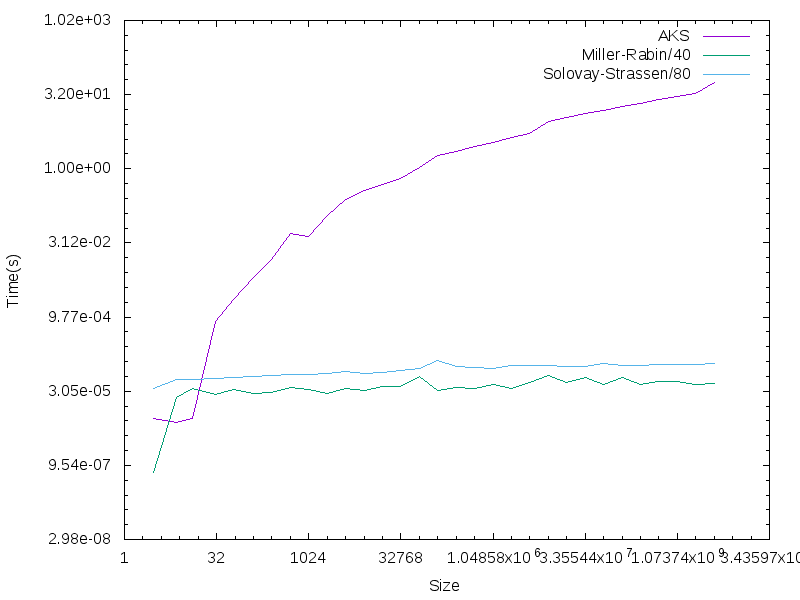
\includegraphics[totalheight=12cm]{img/graphs/aks-probs-primes-mean}
	\caption{Comparación AKS, Miller-Rabin/40 y Solovay-Strassen/80 con números primos}
\end{figure}

Como podemos comprobar, para entradas pequeñas, el algoritmo \textbf{AKS} funciona muy bien e, incluso, superando a los dos test probabilísticos. Sin embargo, vemos que entorno a $32 = 2^5$, el tiempo de ejecución se dispara, lo cual deja claro lo ineficiente del test \textbf{AKS}.\\

El test de \textit{Solovay-Strassen} es un poco peor que el de \textit{Miller-Rabin} porque realizamos el doble de rondas para asegurar probabilidades similares.\\

En conclusión, los tests probabilísticos funcionan mucho más rápido, lo cual es muy útil cuando estamos tratando con números muy grandes, además de que sus posibilidades de dar una respuesta errónea son prácticamente nulas debido a la cantidad de rondas.

\subsection{Potencias de Primos}

Puesto que el primer paso del test \textbf{AKS} es comprobar si la entrada es una potencia perfecta, es interesante ver cómo se comporta frente a los algoritmos probabilísticos con entradas que son potencias de primos.\\

Para esta comparación vamos a usar dos conjuntos distintos de prueba:

\begin{itemize}
	\item Potencias grandes de primos pequeños. En específico, primos de hasta $16$ bits elevados a $100$.
	
	\item Potencias pequeñas de primos grandes. En específico, primos de hasta $256$ bits elevados a $5$.
\end{itemize}

Primero empecemos con las potencias grandes de primos pequeños.

\begin{figure}[H]
	\centering
	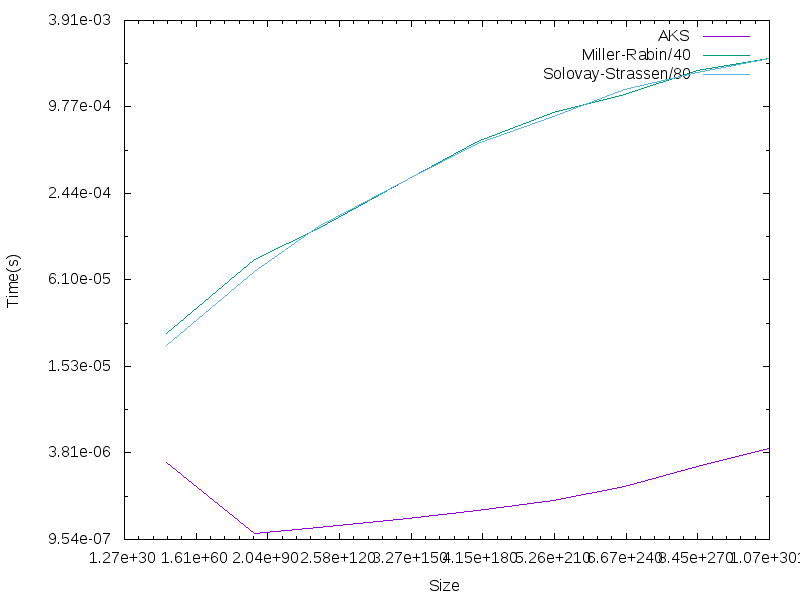
\includegraphics[totalheight=12cm]{img/graphs/aks-probs-powers-100-mean}
	\caption{Comparación AKS, Miller-Rabin/40 y Solovay-Strassen/80 con potencias grandes de primos pequeños}
\end{figure}

Y ahora la gráfica de potencias pequeñas de primos grandes.

\begin{figure}[H]
	\centering
	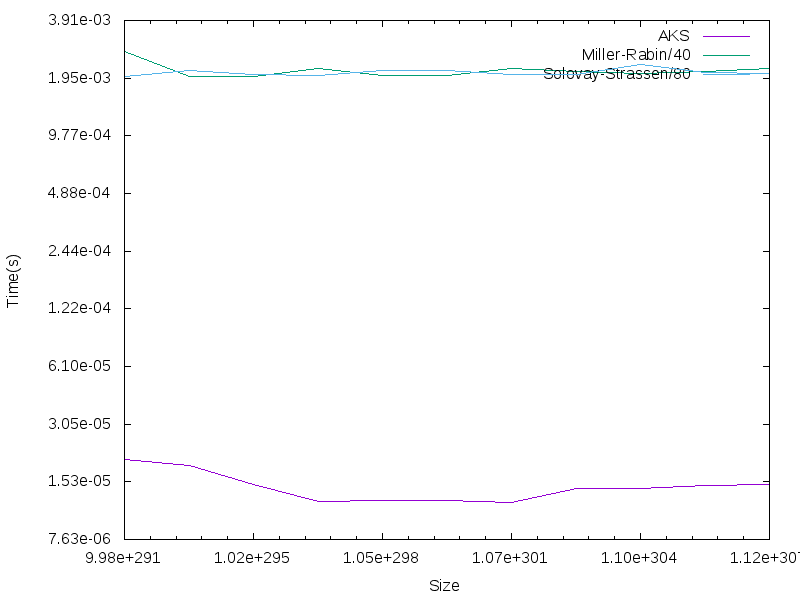
\includegraphics[totalheight=12cm]{img/graphs/aks-probs-powers-5-mean}
	\caption{Comparación AKS, Miller-Rabin/40 y Solovay-Strassen/80 con potencias pequeñas de primos grandes}
\end{figure}

En ambos casos, el análisis es claro. Comprobar si un número es una potencia perfecta es mucho más rápido que aplicar el test de \textit{Miller-Rabin} o el de \textit{Solovay-Strassen}.\\

Puesto que el test \textbf{AKS} maneja las potencias perfectas en el primer paso, y en vista de las gráficas anteriores, concluimos que el test \textbf{AKS} funciona mucho mejor que los test probabilísticos cuando la entrada se trata de una potencia perfecta.

\subsection{Números Compuestos No Potencias de Primos}

Habiendo hecho comparaciones con números primos y potencias de primos, es natural comparar usando números compuestos que no sean potencias de primos. Para ello usaremos números que son producto de dos o más factores primos grandes.\\

Esto nos ayudará a comprobar cómo se comportan los tres tests en los casos más sensibles, es decir, aquellos donde los factores primos son grandes. Determinar correctamente la composición de dichos números es de vital importancia en los protocolos de seguridad como RSA, pues de lo contrario, la seguridad de dicho sistemas se podría ver comprometida.\\

Usaremos distintos conjuntos de prueba:

\begin{itemize}
	\item Compuestos con factores primos grandes de magnitud similar. Por ejemplo, números compuestos que sean producto de un número de $256$ bits y $260$ bits.
	
	\item Compuestos con factores primos de magnitudes distintas. Por ejemplo, números compuestos con factores de $128$ bits y $256$ bits.
\end{itemize}

Vayamos con la gráfica del primer conjunto de prueba.

\begin{figure}[H]
	\centering
	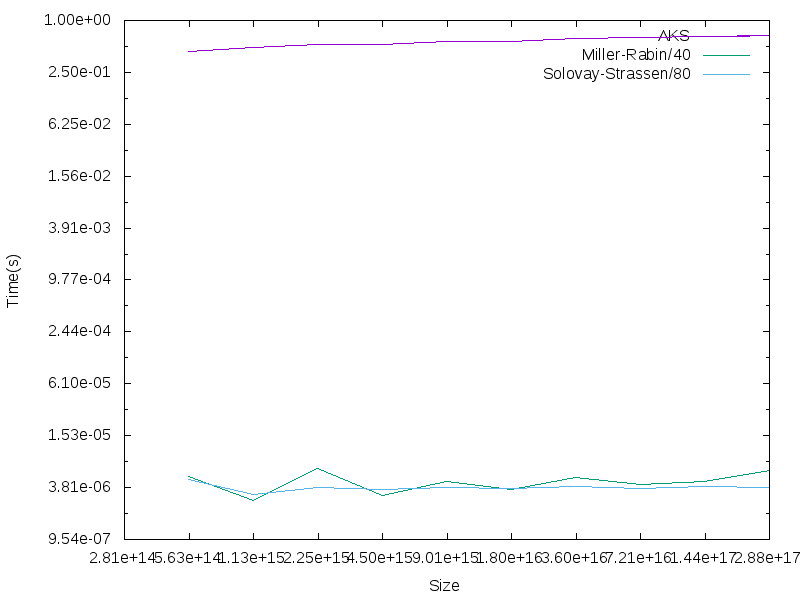
\includegraphics[totalheight=12cm]{img/graphs/aks-probs-comps-16-mean}
	\caption{Comparación AKS, Miller-Rabin/40 y Solovay-Strassen/80 con productos de primos de más de $32$ bits y otro de $16$ bits}
\end{figure}

Ahora veamos la gráfica del segundo.

\begin{figure}[H]
	\centering
	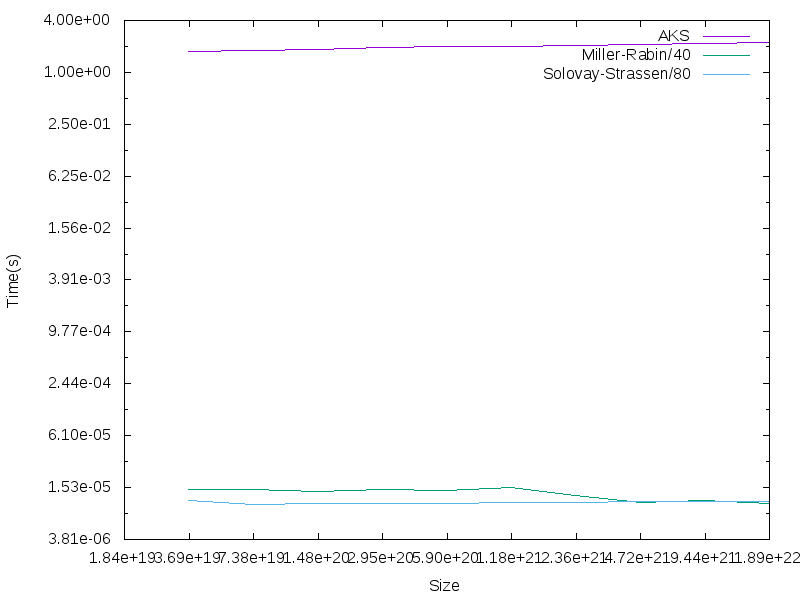
\includegraphics[totalheight=12cm]{img/graphs/aks-probs-comps-32-mean}
	\caption{Comparación AKS, Miller-Rabin/40 y Solovay-Strassen/80 con productos de primos de más de $32$ bits y otro de $32$ bits}
\end{figure}

Aparentemente, podemos comprobar que las gráficas son idénticas y que el tamaño de los factores no afecta en cómo se comportan el test \textbf{AKS} respecto de los otros.\\

Volvemos a comprobar, al igual que ya pasó con el caso en que la entrada eran primos, que el algoritmo \textbf{AKS} es bastante peor que sus contrapartes probabilísticas.

\section{Conclusión}

Como conclusión final de este apartado, y vistas las observaciones realizadas en esta comparación con los algoritmos probabilísticos, es que el algoritmo \textbf{AKS}, aún siendo general, polinómico, determinista e incondicional, es excesivamente lento para entradas no muy grandes, lo cual hace inviable su uso en otras aplicaciones de la criptografía.\\

Los algoritmos probabilísticos, aunque su respuesta no sea determinista, son suficientemente fiables en la mayoría de los casos, y su tiempo de ejecución los hace extremadamente convenientes cuando se trata de números con una gran cantidad de cifras.

\endinput
%------------------------------------------------------------------------------------
% FIN DEL CAPÍTULO. 
%------------------------------------------------------------------------------------


% --------------------------------------------------------------------
% APPENDIX: Opcional
% --------------------------------------------------------------------

\appendix % Reinicia la numeración de los capítulos y usa letras para numerarlos
\pdfbookmark[-1]{Apéndices}{appendix} % Alternativamente podemos agrupar los apéndices con un nuevo \part{Apéndices}

% !TeX root = ../libro.tex
% !TeX encoding = utf8

\chapter{Primer apéndice}\label{ap:apendice1}

Los apéndices son opcionales.

Archivo: \texttt{apendices/apendice01.tex}

\endinput
%------------------------------------------------------------------------------------
% FIN DEL APÉNDICE. 
%------------------------------------------------------------------------------------

% Añadir tantos apéndices como sea necesario 

% --------------------------------------------------------------------
% GLOSARIO: Opcional
% --------------------------------------------------------------------

% !TeX root = ../libro.tex
% !TeX encoding = utf8

\chapter*{Glosario}
\addcontentsline{toc}{chapter}{Glosario} % Añade el glosario a la tabla de contenidos

\begin{description}
	\item[$\N$] Conjunto de números naturales con el $0$ incluido.
	
	\item[$\Z$] Conjunto de números enteros.
	
	\item[$\R$] Conjunto de números reales.
	
	\item[$\C$] Conjunto de números complejos.
	
	\item[$|C|$] Cantidad de elementos distintos en el conjunto $C$ o su cardinal.
	
	\item[$\sum$] Sumatoria de varios elementos.
	
	\item[$\prod$] Producto de varios elementos.
	
	\item[$\int_{a}^{b}$] Integral definida en el intervalo $[a, b]$.
	
	\item[$f'(x)$] Derivada de la función $f(x)$.
	
	\item[$(a, b)$] Máximo Común Divisor de $a$ y $b$.
	
	\item[${[a, b]}$] Mínimo Común Múltiplo de $a$ y $b$.
	
	\item[$LCM(m)$] Mínimo Común Múltiplo de los $m$ primeros números.
	
	\item[$res(a; b)$] Resto de dividir $a$ entre $b$.
	
	\item[$a\mid b$] El número $a$ divide a $b$.
	
	\item[$a\nmid b$] El número $a$ no divide a $b$.
	
	\item[$\phi(n)$] Función $\phi$ de Euler.
	
	\item[$\mathcal{U}(A)$] Grupo formado por las unidades del anillo $A$.
	
	\item[${A[x]}$] Anillo de polinomios con coeficientes en el anillo $A$.
	
	\item[$or(a)$] Orden del elemento $a$ de un grupo $G$, es decir, el menor $k$ tal que $a^k = 1$.
	
	\item[$ord_n(a)$] Orden de $a$ módulo $n$, es decir, el menor $k$ tal que $a^k \equiv 1 \mod(n)$.
	
	\item[$\Phi_n$] $n$-ésimo polinomio ciclotómico.
	
	\item[$\binom{n}{k}$] Binomio de $n$ sobre $k$.
	
	\item[$n!$] Producto de los primeros $n$ números o factorial de $n$.
	
	\item[$\left(\frac{a}{b}\right)$] Símbolo de Jacobi/Legendre de $a$ y $b$.
	
	\item[$a \equiv b \mod(n)$] Congruencia de $a$ con $b$ módulo $n$.
	
	\item[$\mathbb{F}_q$] Cuerpo finito de tamaño $q$ potencia de un primo.
	
	\item[$O(f(n))$] Complejidad asintótica máxima.
	
	\item[$\Omega(f(n))$] Complejidad asintótica mínima.
	
	\item[$\Theta(f(n))$] Complejidad asintótica exacta.
	
	\item[$O^\sim(f(n))$] Equivalente a $O(f(n)poly(\log(f(n)))$ donde $poly(n)$ es un polinomio.
	
	\item[$\lfloor x \rfloor$] Parte entera por deceso de $x$.
	
	\item[$\lceil x \rceil$] Parte entera por exceso de $x$.
	
	\item[$\log(n)$] Logaritmo en base $2$ de $n$.
	
	\item[$\ln(n)$] Logaritmo natural o en base $e$ de $n$.
	
	\item[AKS] Algoritmo desarrollado por \textit{Agrawal}, \textit{Kayal} y \textit{Saxena}.
	
	\item[FFT] Transformada Rápida de Fourier.
	
	\item[DFT] Transformada Discreta de Fourier.
	
	\item[GCC] GNU C Compiler.
	
	\item[Clang] LLVM C/C++ Lang Compiler.
	
	\item[MSVC] Microsoft Visual C and C++ Compiler.
	
	\item[CMake] Generador de sistemas de compilación (Meta Build System).
	
	\item[Conan] Manejador de paquetes de C y C++
	
	\item[C++] Lenguaje de Programación C++.
	
	\item[GMP] GNU Mutiprecision Library.
	
	\item[MPFR] GNU Multiprecision Floating-Point Reliable Library.
	
	\item[NTL] Number Theory Library.
\end{description}
\endinput
 

% -------------------------------------------------------------------
% BACKMATTER
% -------------------------------------------------------------------

\backmatter % Desactiva la numeración de los capítulos
\pdfbookmark[-1]{Referencias e Índices}{BM-Referencias}

% BIBLIOGRAFÍA
%-------------------------------------------------------------------

\setbibpreamble{Las referencias se listan por orden alfabético. Aquellas referencias con más de un autor están ordenadas de acuerdo con el primer autor.\par\bigskip}
\bibliographystyle{alpha} 
\begin{small} % Normalmente la bibliografía se imprime en un tamaño de letra más pequeño.
\bibliography{library.bib}
\end{small}


% ÍNDICE TERMINOLÓGICO  (Opcional) 
%------------------------------------------------------------------- 

% Para incluir el índice terminológico es necesario descomentar los siguientes comandos. Incluir un índice terminológico es opcional

% \cleardoublepage 
% \begin{footnotesize} % Normalmente el índice se imprime en un tamaño de letra más pequeño.
% \printindex 
% \end{footnotesize}

\end{document}
